\chapter{Nuclear Models}

\section{Introduction}

In the following, it is worth to make a discussion about the nuclear models that are used by theoreticians in order to describe phenomena that are specific to rotating nuclei and high-spin regime. Since the focus of this work emerges from a \emph{class} of properties that usually apply to the high-spin region (but this does not necessarily also imply a high-energy region), it makes sense to give an insight in the tools that fit the best the underlying effects.

\section{Shell model}

The fact that an atomic nucleus can have a structure that behaves rather similarly as its \emph{parent} (i.e., the atom) in terms of changing the number of constituents, has been enforced by the experimental observations that were done across time. The sharp and discrete discontinuities of nuclear properties, such as the nucleon separation energy, point to the fact that nucleus can be explained through the existence of \emph{shells}. Some examples of observations which indicate this are:
\begin{itemize}
    \item When adding a nucleon to a nucleus, there are certain places where the \emph{binding energy} of the next nucleon becomes considerably smaller than the previous one. 
    \item Separation energies for both the protons and neutrons suffer drastic changes, having strong deviations from the predictions of the semi-empirical mass formula \cite{weizsacker1935theorie}, the discontinuities being represented by major shell closures (complete filling) \cite{krane1991introductory}.
    \item The neutron absorption cross-section has a substantial decrease in value at the neutron magic numbers
    \item Great abundance of nuclides where $Z$ and $N$ are magic numbers.
\end{itemize}

The sudden discontinuities occur at specific values of the proton $Z$ and neutron $N$ numbers: these are called \emph{magic numbers}. Currently, these magic numbers correspond to $Z$ or $N=2,8,20,28,50,82,126$, and they represent the so-called major shells. There are also two \emph{weakly magic numbers}: 40 and 64.

One can examine the values for the first excited states $2^+$ that are shown in Figs. \ref{e2plus_proton}, \ref{e2plus_neutron}. Indeed, these values show some peaks, each peak corresponding to a particular magic number. This results are part of the work of Raman et al \cite{raman2001transition}, where the transition probabilities from the ground state to the first-excited $2^+$ state in even-even nuclei were evaluated.

\begin{figure}
    \centering
    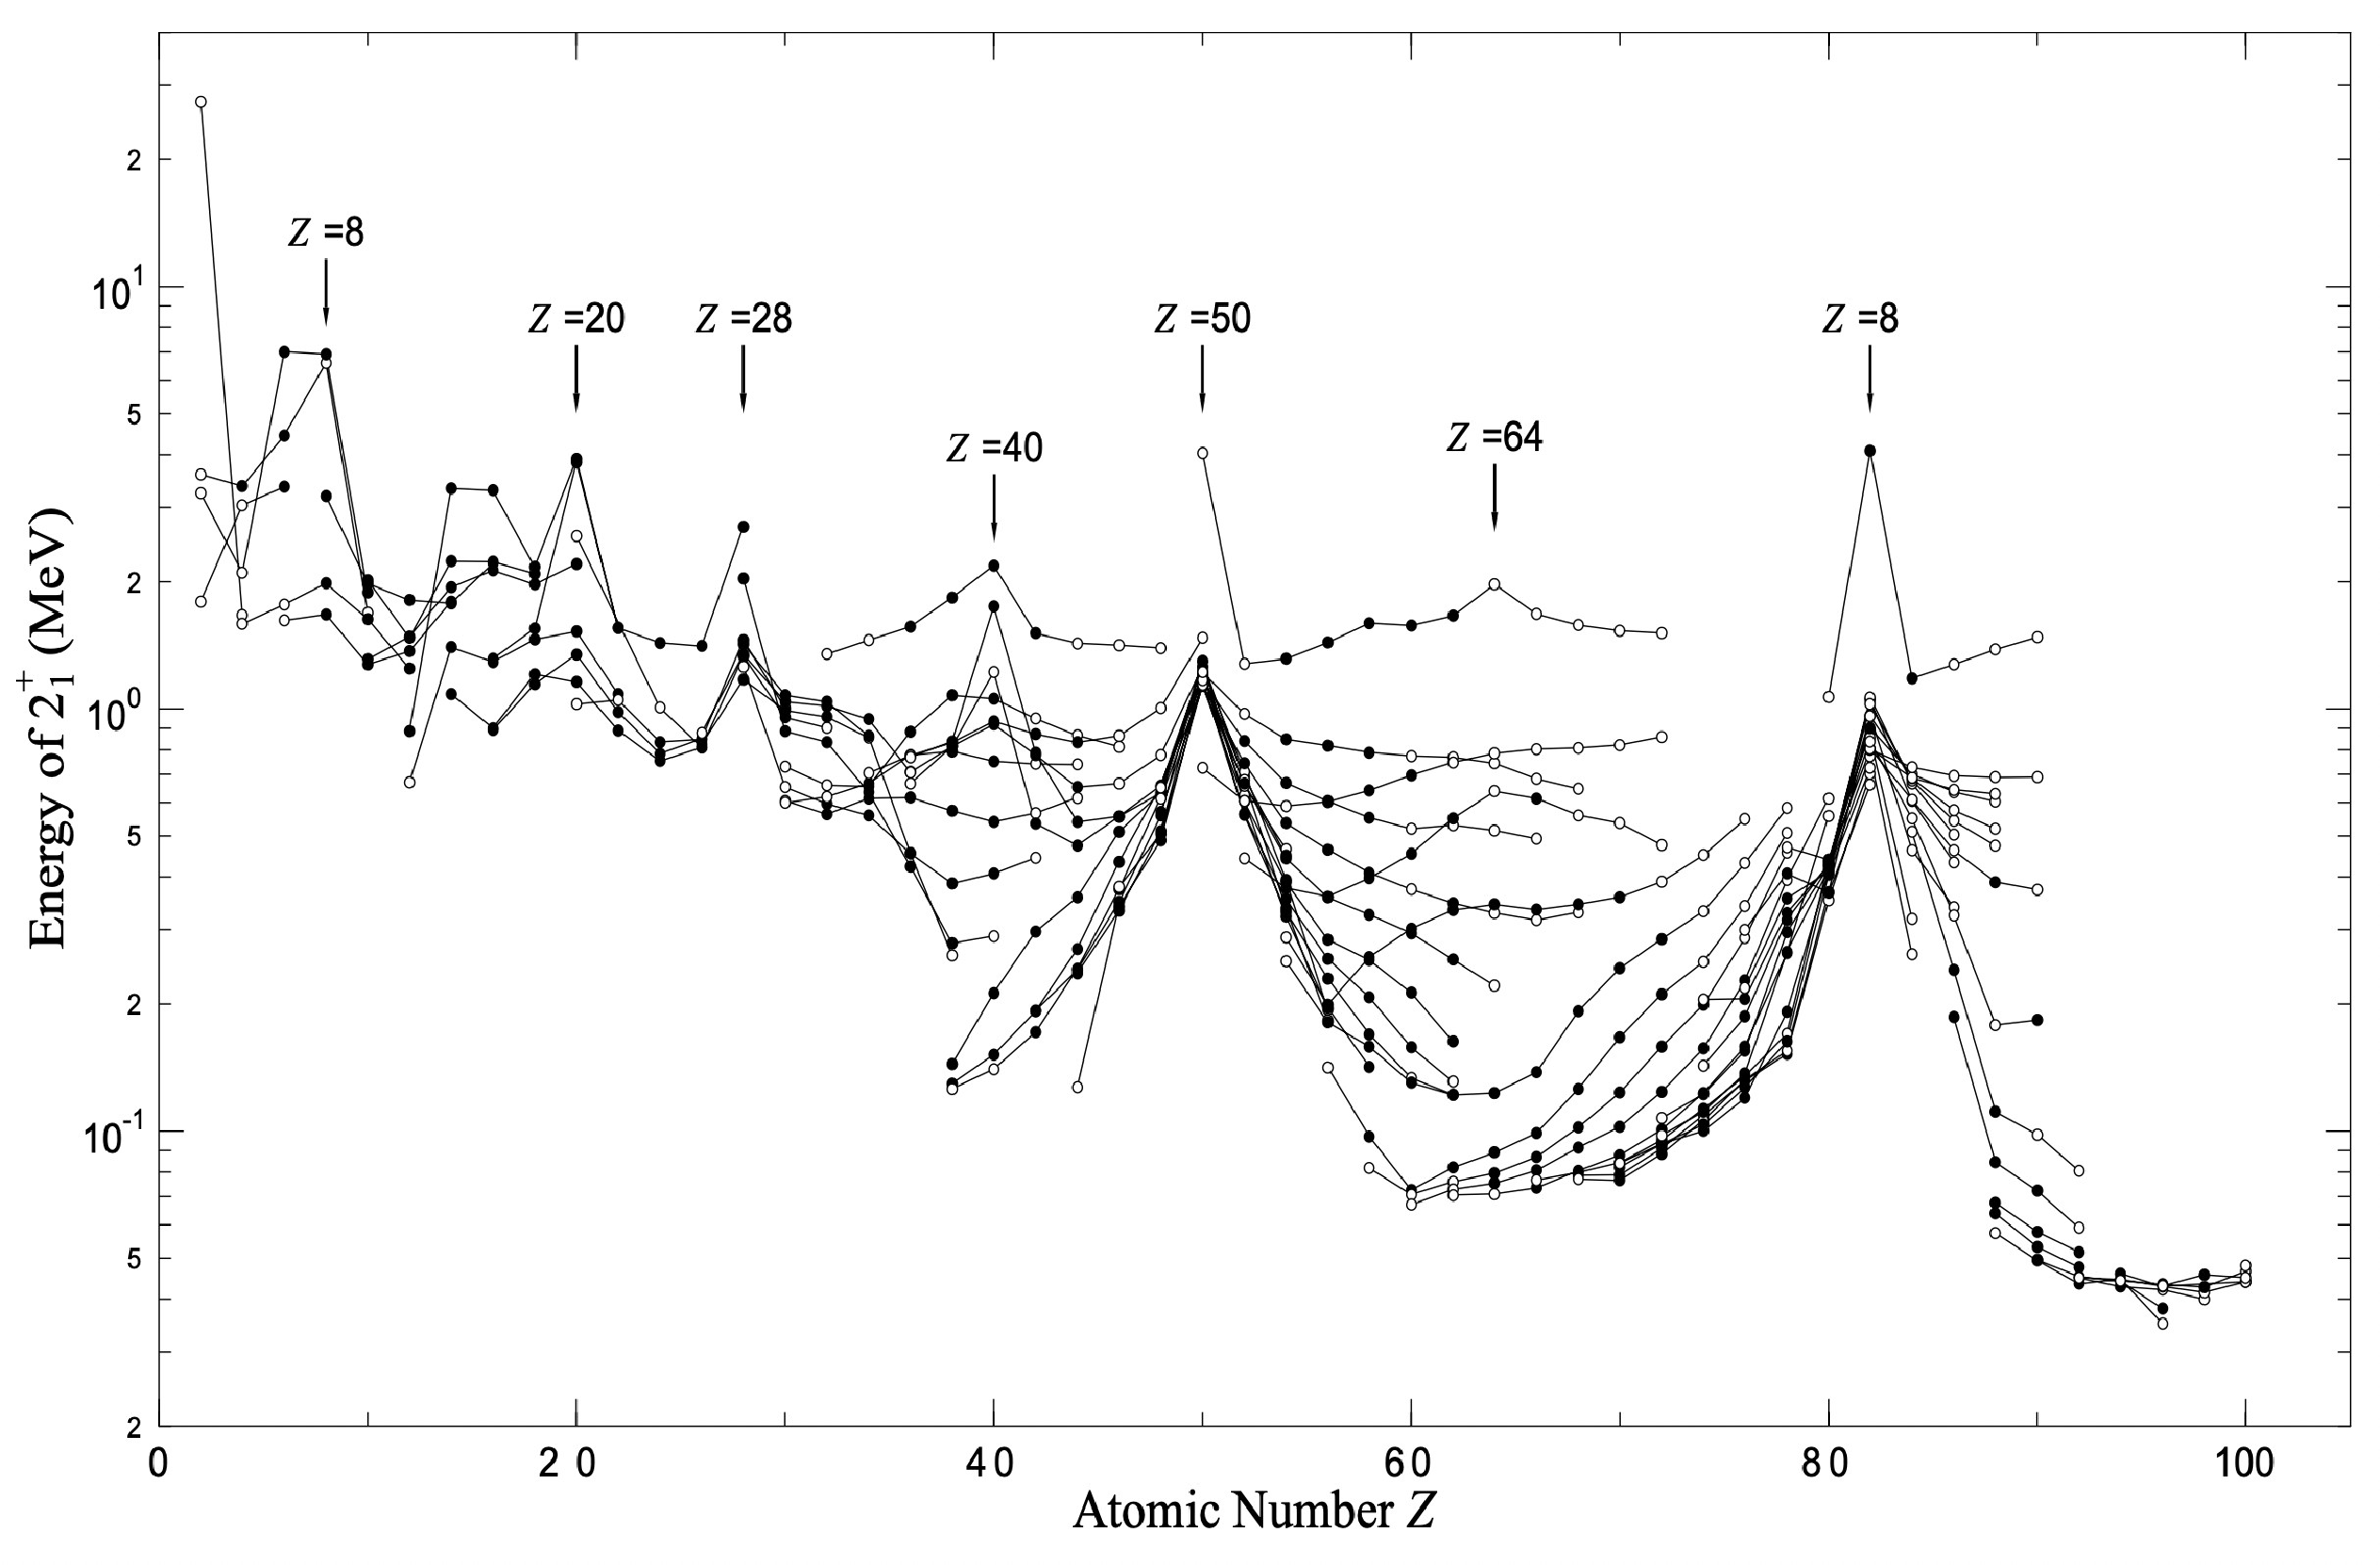
\includegraphics[scale=0.33]{Chapters/Figures/E2plus_proton.pdf}
    \caption{The first excited energy states $2^+$ of nuclei with even $Z$ and $N$ graphically represented with respect to the proton number. Each line represents a set of isotopes. Figure taken from Ref. \cite{matta2017exotic}.}
    \label{e2plus_proton}
\end{figure}

\begin{figure}
    \centering
    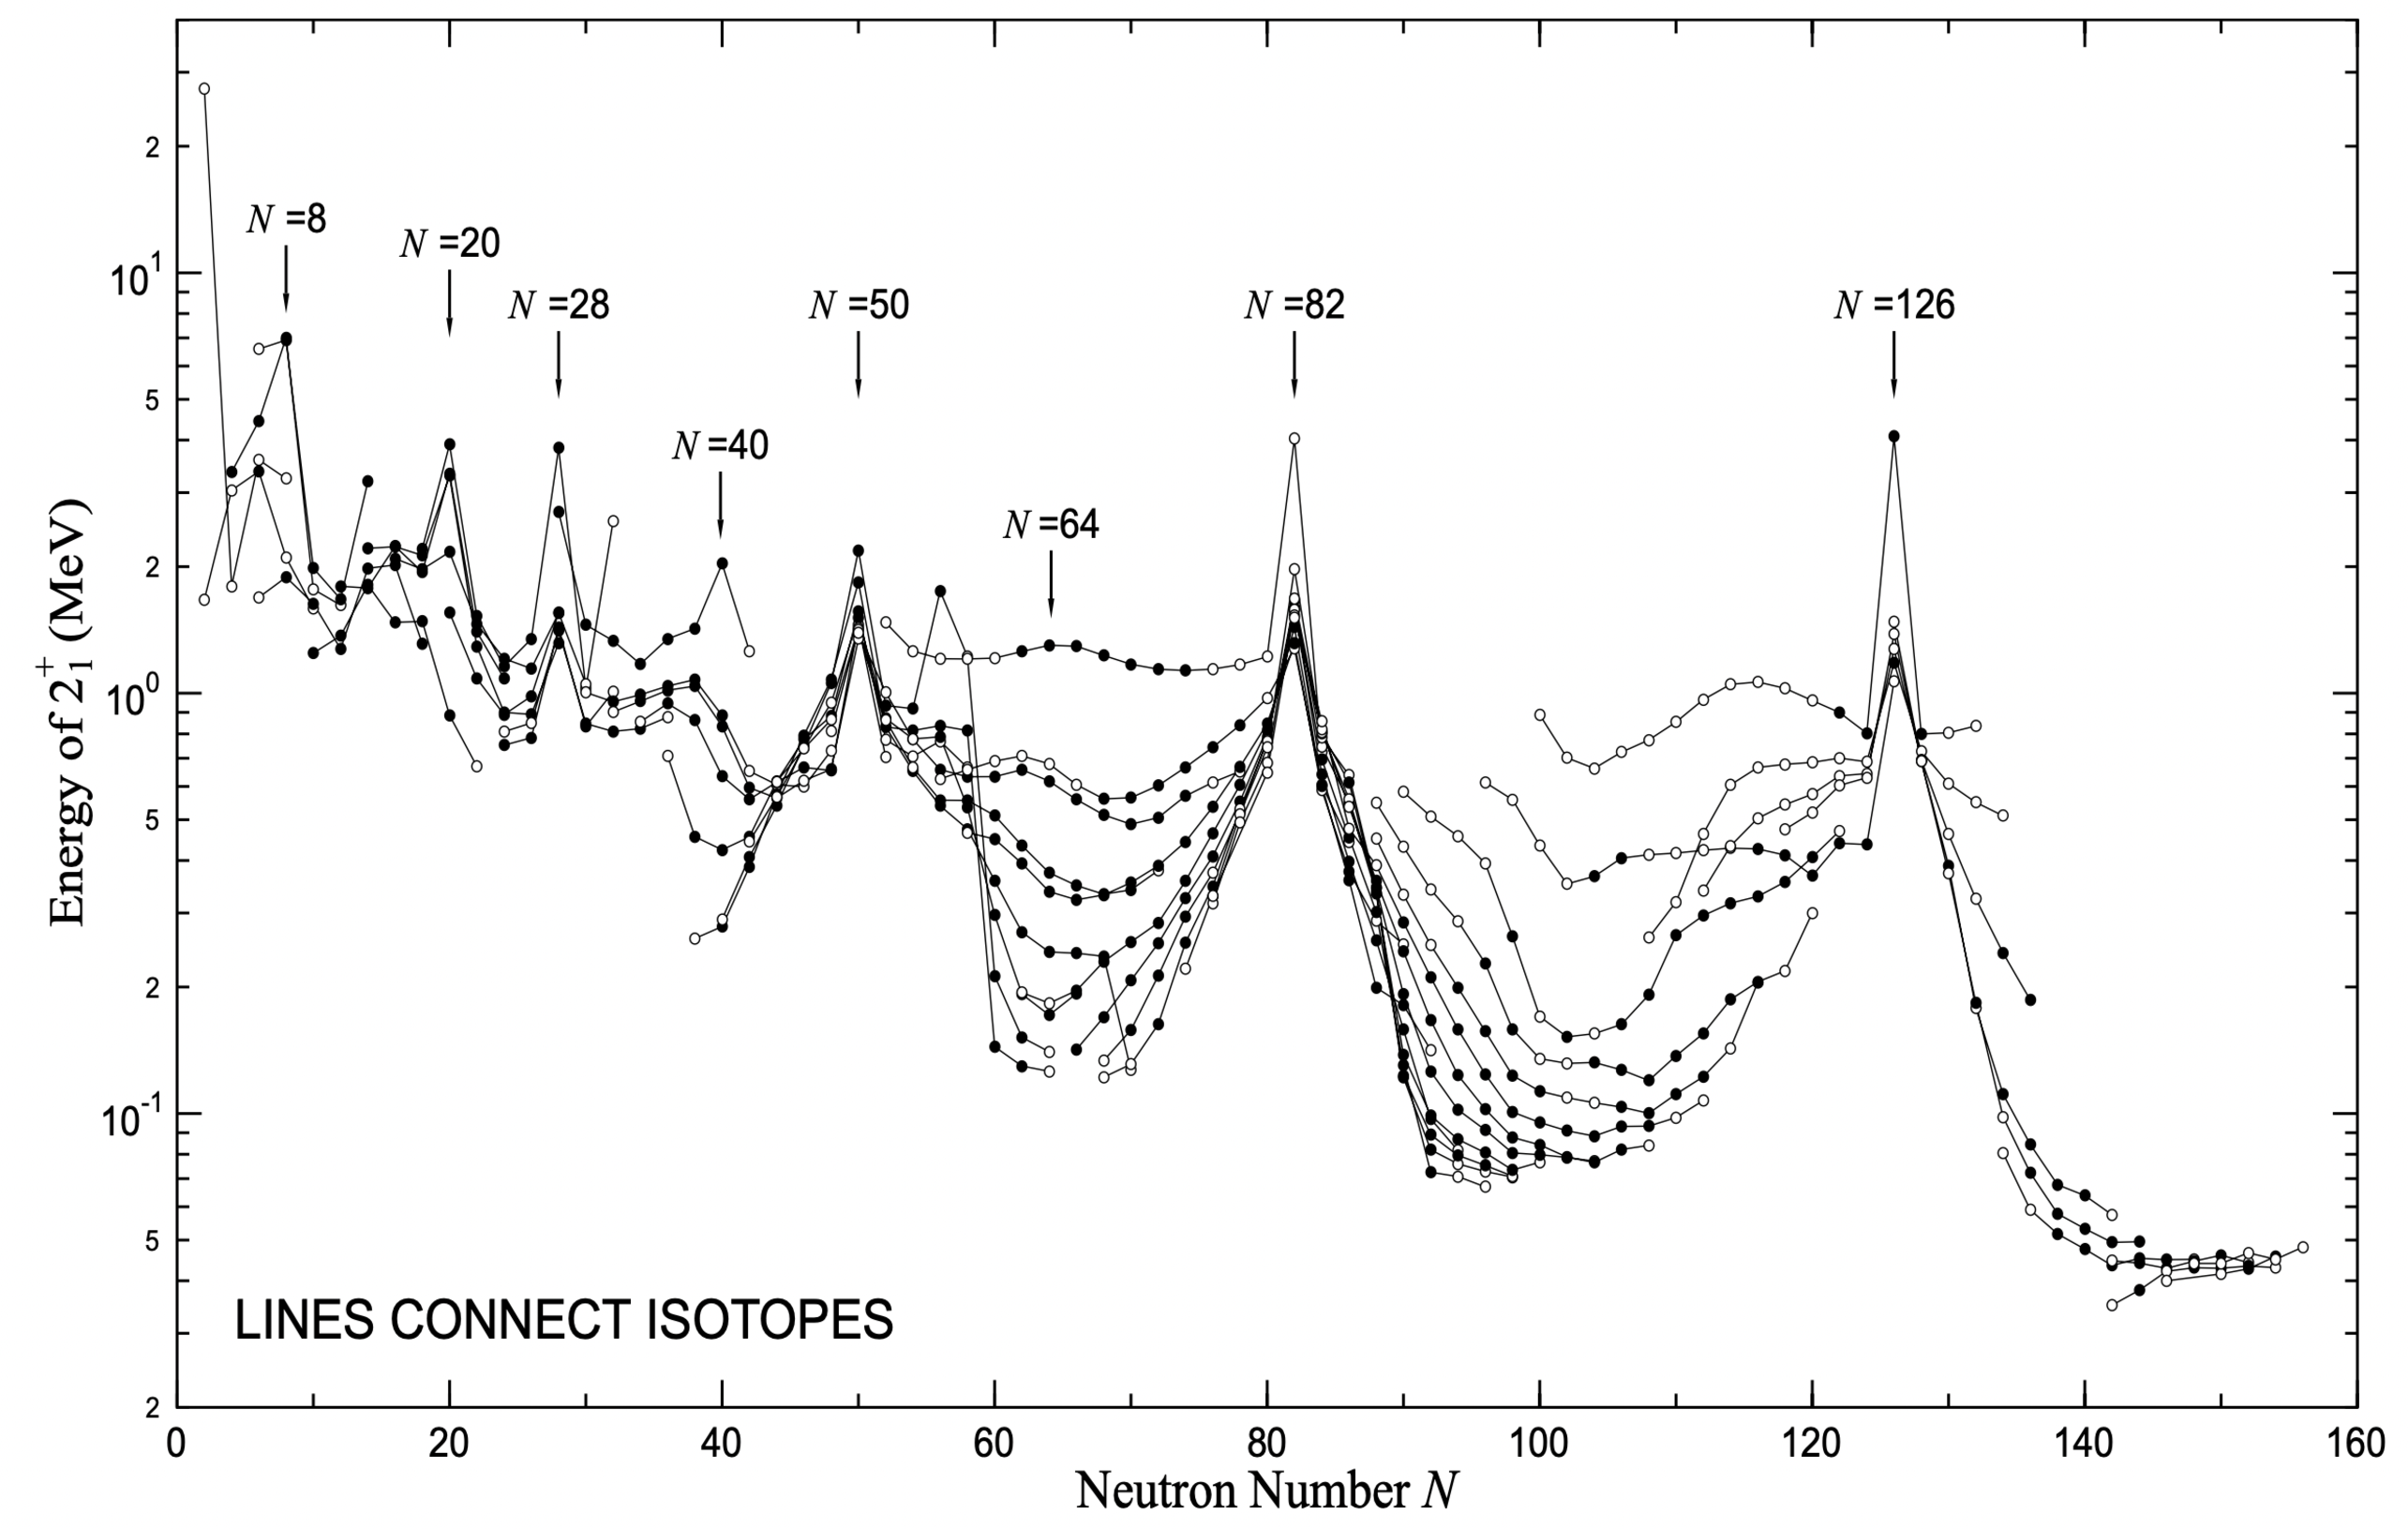
\includegraphics[scale=0.33]{Chapters/Figures/E2plus_neutron.pdf}
    \caption{The first excited energy states $2^+$ of nuclei with even $Z$ and $N$ graphically represented with respect to the neutron number. Each line represents a set of isotopes. Figure taken from Ref. \cite{matta2017exotic}.}
    \label{e2plus_neutron}
\end{figure}

The shell model starts from the basic assumption that the nucleus is a \emph{mean-field potential}, that is a potential for which the motion of a single nucleon is caused by all the other nucleons (the nucleon is moving inside an average potential generated by all the other constituents of the nucleus). Of course, all the nucleons that are under the influence of such a mean field potential occupy the energy levels which correspond to a series of (sub)shells that agree with the Paul exclusion principle. Having a general expression for the potential that properly reproduces all the magic numbers (and the observed nuclear properties) is the main goal.

Since the model starts from the concept of independent (non-interacting) particle motion within an average potential, finding each energy will be equivalent of solving the Schrödinger equation:
\begin{align}
    -\frac{\hbar^2}{2m}\nabla ^2\psi_i(r)+V(r)\psi_i(r)=e_i\psi_i(r)\, 
    \label{schrodinger-single-particle-eq}
\end{align}
where $e_i$ represents the energy (eigenvalue) and $\psi_i$ represents the wave-function (eigenstates), while $V(r)$ is the nuclear potential whose expression must be evaluated.

The choice of $V(r)$ will be dictated by the reproduction of various experimental data (such as nuclear saturation, scattering, nuclear reactions, and so on). For the motion of an independent particle, an obvious first attempt would be the \emph{simple harmonic oscillator} (SHO), which has the known expression:
\begin{align}
    V(r)=\frac{1}{2}m(\omega_i r)^2\ ,
    \label{harmonic-potential}
\end{align}
with $\omega_i$ as the frequency of the basic harmonic-like motion of the particle in the nucleus. With Eq. \ref{harmonic-potential}, the motion of the nucleon has a straightforward expression:
\begin{align}
    \frac{\hbar^2}{2m}\nabla^2\psi_i(r)+\frac{1}{2}m(\omega r)^2\psi_i(r)=e_i\psi_i(r)\ .
\end{align}

This Schrödinger equation has its energy eigenvalues under to form:
\begin{align}
    e_N=\left(N+\frac{3}{2}\right)\hbar\omega\ ,
\end{align}
where $N$ is the number of oscillator quanta which describes each major shell (also called the \emph{principal quantum number}). One should keep in mind that such an expression is typical for a three-dimensional and isotropic harmonic oscillator. The principal quantum number $N$ is furthermore defined as:
\begin{align}
    N=2(n-1)+l\ ,
\end{align}
with $n$ and $l$ being the \emph{radial} quantum number and \emph{orbital angular momentum} quantum number, respectively, taking values $n=1,2,3,\dots$ and $l=0,1,2,\dots,n-1$. In this first approximation, all the levels with the same principal quantum number $N$ are \emph{degenerate}, with a maximal degeneracy given by $2(2l+1)$. However, by using only the SHO term as the expression of $V(r)$, only the first three magic numbers are reproduced, meaning that some additional term(s) might be needed in order to consistently obtain the series of magic numbers.

A next step is to use the fact that the experimentally observed short range of the strong nuclear force: the steepness of the SHO can be corrected with an \emph{attractive} term proportional to $l$-squared. This acts as a centrifugal term which provides an angular momentum barrier, lifting the degeneracy between the levels with the same principal quantum number $N$ and different values for the orbital angular momentum $l$. This SHO+$l^2$ step is still not enough though. The last step is to add a so-called \emph{spin-orbit} coupling term of the form $\vec{l}\cdot\vec{s}$. 
% This last term is enough to reproduce all the magic numbers and the experimentally measured quantities that are relevant to the shell model itself.
This term comes from the consideration that the nucleon-nucleon interaction has a spin dependence, and the potential depends on the intrinsic spin $s$ ($\vec{s}$) and the orbital angular momentum $l$ ($\vec{l}$) of a nucleon. Since $\vec{j}=\vec{l}+\vec{s}$, two possible states emerge from a single value of $l$ (depending on wether $\vec{s}$ is parallel or anti-parallel to $\vec{l}$). The final expression of the terms SHO+$\vec{l}^2$+$\vec{l}\cdot\vec{s}$ will consist in the \emph{Modified Harmonic Oscillator} (HMO).
\begin{align}
    V(r)=\frac{1}{2}(\omega r)^2+B\ \vec{l}^2+A\ \vec{l}\cdot\vec{s}\ .
    \label{modified-harmonic-oscillator-eq}
\end{align}

For the sake of simplicity, the centrifugal term will be denoted within formulas without the vector symbol. Since the intrinsic spin of a nucleon is $s=1/2$, for a given value of $l$, there can be two values for the \emph{total angular momentum} (a.m.) $j=l\pm1/2$: one for each spin orientation with respect to the direction of the orbital a.m. Moreover, for each value of $l=0,1,2,3,4,\dots$, there is a similar notation $l=s,p,d,f,g,\dots$, respectively. Regarding the spectroscopic notation, usually, the value of $j$ is considered as a subscript; $nl_j$ (for example $1p_{1/2}$ and $1p_{3/2}$). What it is worth mentioning is that for high enough shells, there can be splittings between $j+1/2$ and $j-1/2$ that are large enough to lower the $j+1/2$ state from one oscillator shell $n$ to one located below $n-1$. These types of levels are called \emph{intruder states} and they have opposite parity $\pi=(-1)^l$ with respect to the shell that these levels will occupy.

Going back to the expression of the $\vec{l}\cdot\vec{s}$ term from Eq. \ref{modified-harmonic-oscillator-eq} and denoting it with $V_{ls}(r)$, it is shown by Casten \cite{casten2000nuclear} that its contribution to the total potential can be regarded as a surface effect. Due to this, its form can be expressed as a function that depends on the radial coordinate as such \cite{casten2000nuclear}:
\begin{align}
    V_{ls}(r)=-a_{ls}\frac{\partial V(r)}{\partial r}\vec{l}\cdot\vec{s}\ ,
\end{align}
where $V(r)$ is the expression for a central potential and $a_{ls}$ is a strength constant.
% Indeed, in the work of Casten \cite{casten2000nuclear}, it is stated that if in the nucleus, the spin-orbit forces were large enough, then there should be an overall preference for nucleons with spins aligned parallel their orbital a.m. other than the opposite alignment, making the nucleons with anti-parallel spins to not be surrounded by an equal number of nucleons with all spin orientations.

Now that an expression for the nuclear potential that is able to reproduce all the magic numbers has been formulated, it is also possible to formulate the total energy of a single-particle within the average potential that is generated by all the other nucleons within the nucleus. Thus, the Hamiltonian of this simple system (the modified oscillator) can be formulated as such:
\begin{align}
    H&=-\frac{\hbar^2}{2m}\nabla^2+V_\text{SHO}+(l^2)_\text{term}+(\vec{l}\cdot\vec{s})_\text{term}=-\frac{\hbar^2}{2m}\nabla^2+V_\text{MHO} , \nonumber\\
    H&=-\frac{\hbar^2}{2m}\nabla^2+\frac{1}{2}m(\omega r)^2+Bl^2+A\vec{l}\cdot\vec{s}\ .
\end{align}

The evolution from each term in the shell-model potential (that is the first approximation as a SHO, then SHO+$l^2$, and finally SHO+$l^2+\vec{l}\cdot\vec{s}$ or modified oscillator potential) is illustrated in Fig. \ref{energy-levels-mho}, where it can be seen how each extra term introduces a new degeneracy within the energy states, with the complete reproduction of the magic numbers in the third column. Moreover, the \emph{intruder} levels can be observed, where levels with $j=l+1/2$ from a particular $n$ are so low, that they lie below an $n-1$ adjacent level.
\begin{figure}
    \centering
    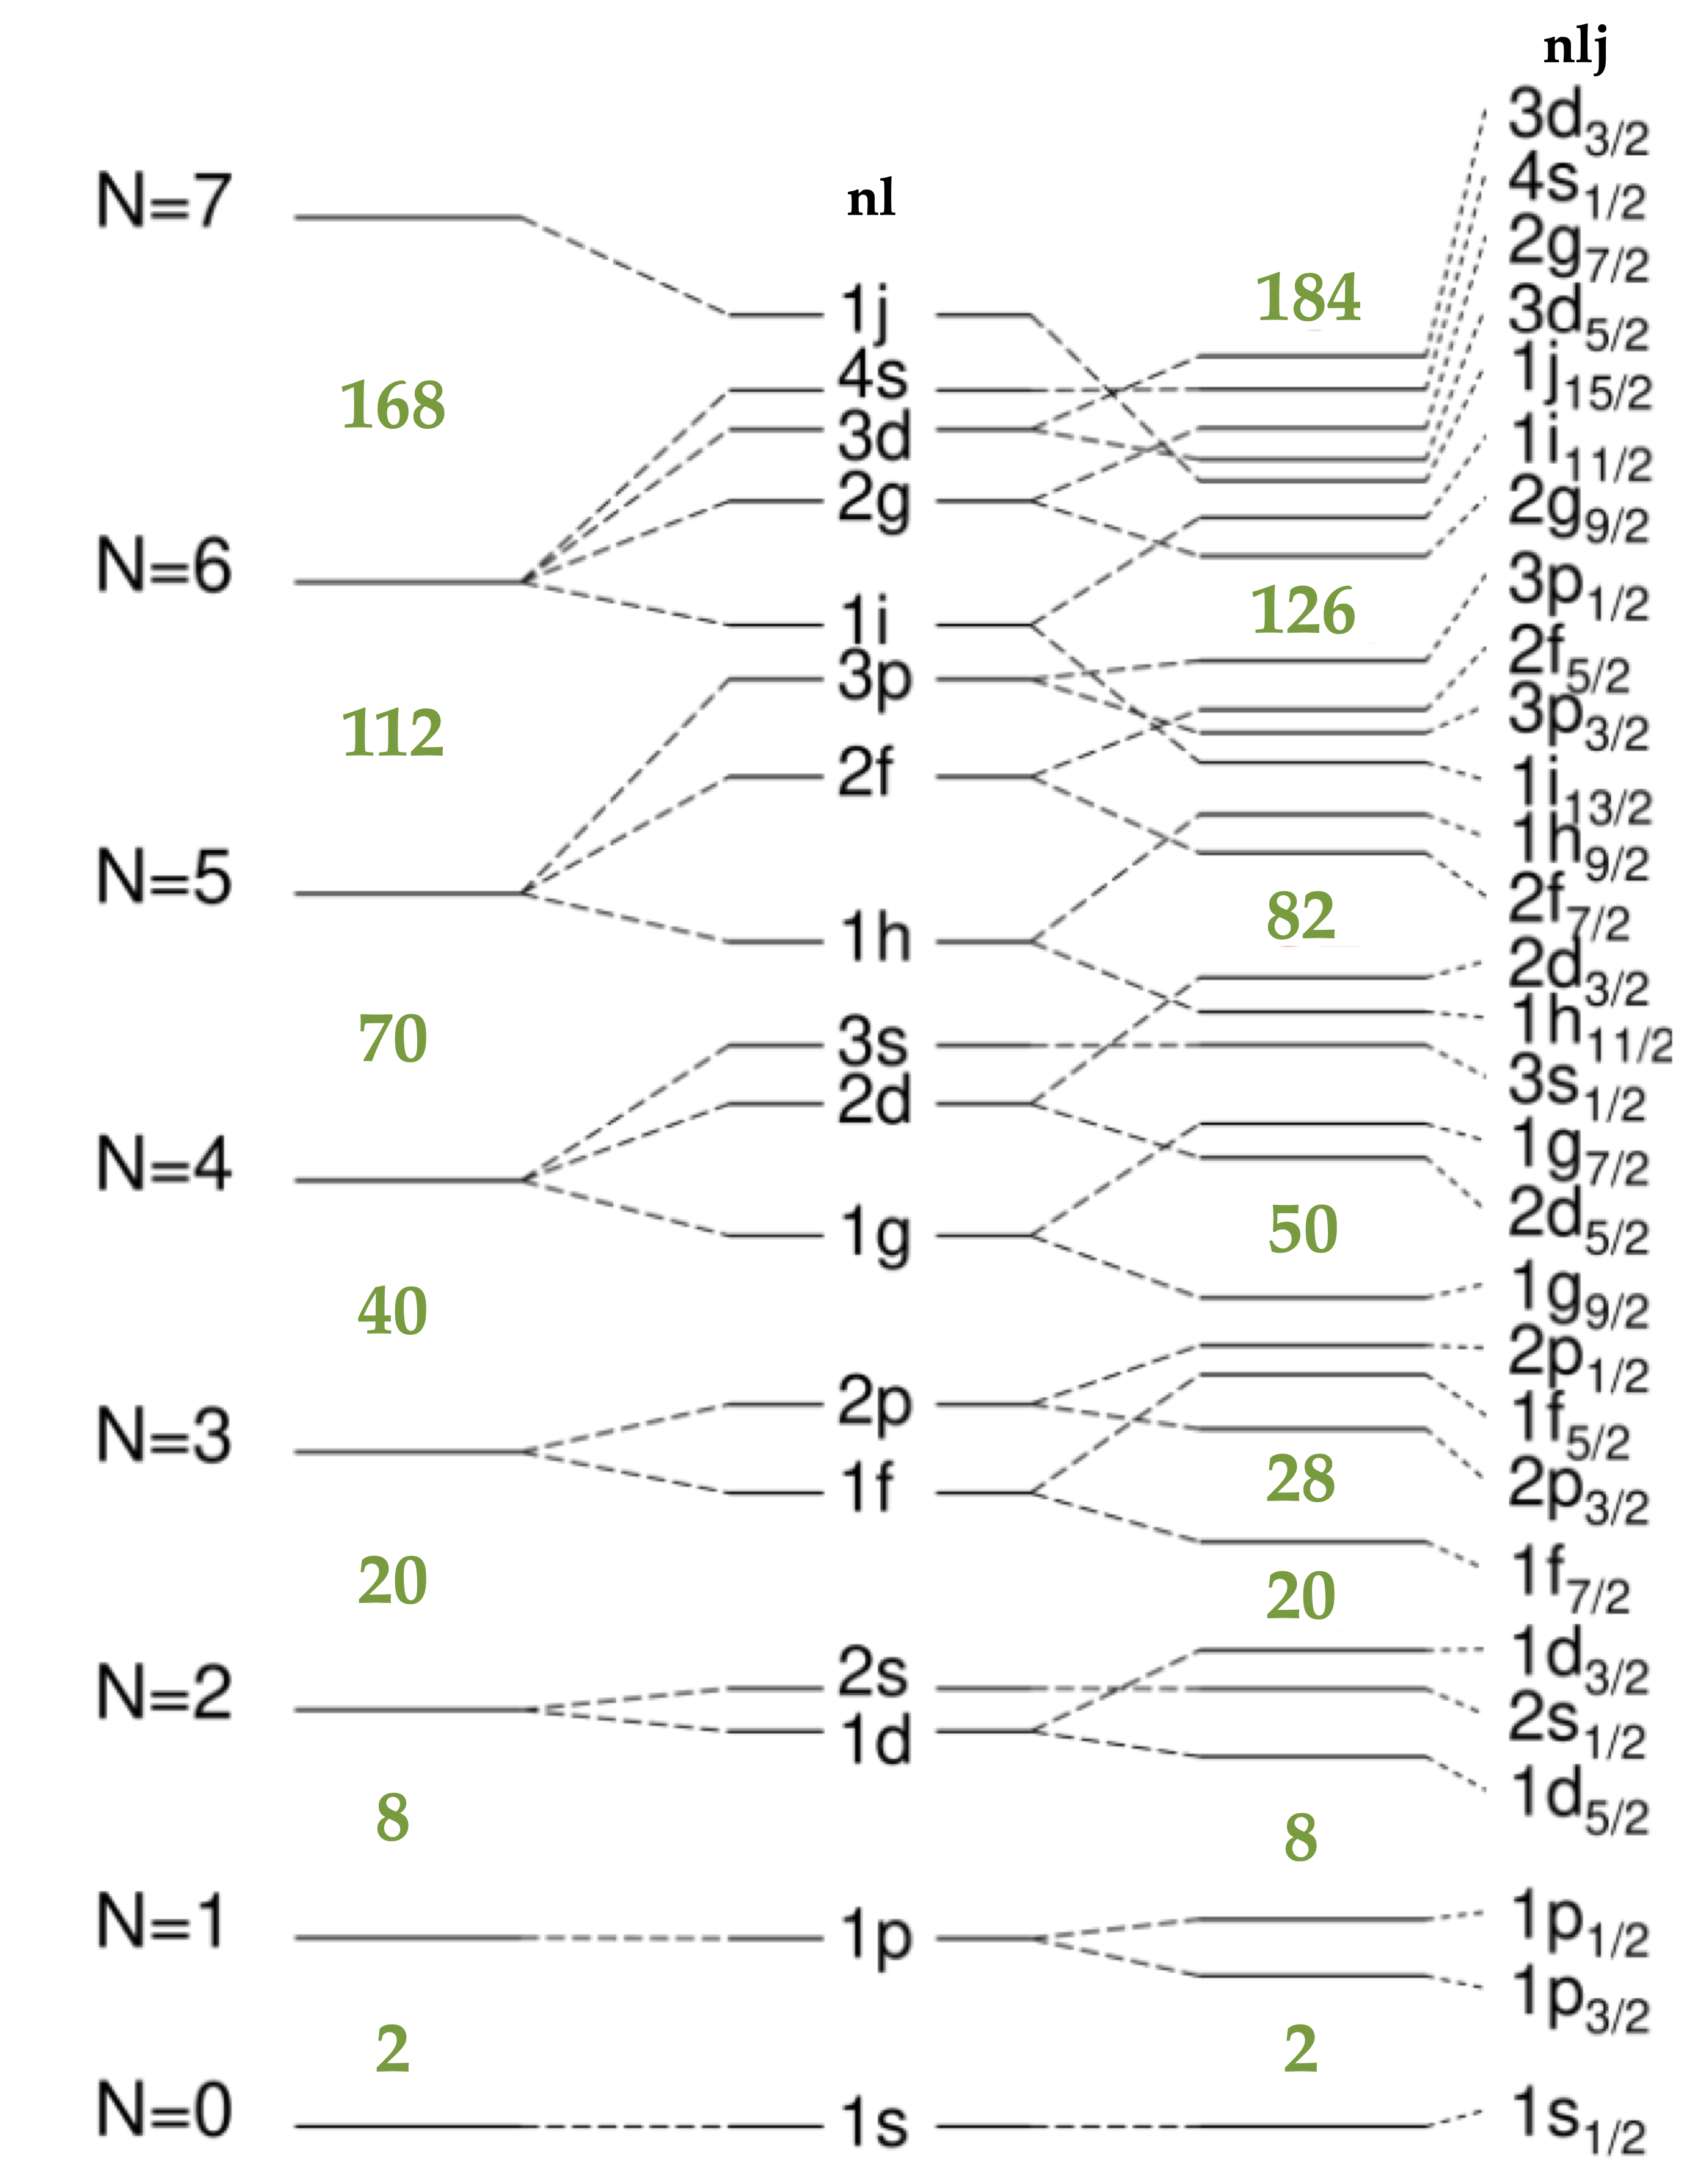
\includegraphics[scale=0.12]{Chapters/Figures/SM_level_scheme.png}
    \caption{The energy levels obtained via calculation of the shell model potential using the simple oscillator (SHO), the SHO amended with a centrifugal term $l^2$, and finally the modified oscillator (MHO) that contains a spin-orbit term. The `correct' magic numbers are the ones in the right-most column. Figure is adapted from Refs. \cite{matta2017exotic},\cite{krane1991introductory}.}
    \label{energy-levels-mho}
\end{figure}

Another, more realistic potential that can be used in order to reproduce the specific shell model calculation is the so-called Woods-Saxon potential. Because of the short-range character of the strong nuclear force, it is safe to assume that this potential should behave in the same manner as the density distribution of the nucleons. Since for medium and heavy nuclei, the Fermi-like functions (distributions) are the ones that best fit the experimentally measured data, this potential should have the following form \cite{woods1954diffuse}:
\begin{align}
    V_\text{ws}(r)=-\frac{V_0}{1+e^{\frac{r-R_0}{a}}}\ .
    \label{woods-saxon-potential}
\end{align}
This mean-field potential contains the terms $V_0$ that represents the depth of the potential ($\approx 50$ MeV, in order to reproduce the experimental separation energies for the nucleons), the surface thickness $a$ (also called the diffuseness parameter, giving information about how fast the potential drops to zero) with a value of approximately $0.5$ fm, while $R_0$ is the nuclear radius with $R_0=r_0A^{1/3}$ and $r_0=1.2$ fm. The nature of this potential is of \emph{central type} and, unfortunately, Eq. \ref{woods-saxon-potential} in its pure form is not enough the reproduce the higher magic numbers. As such, the addition of a spin-orbit term, similarly as in the case of MHO potential, is required \cite{martin2017particle}: 
\begin{align}
    V_\text{total}=V_\text{ws}^\text{central}+V_{ls}(r)\vec{l}\cdot\vec{s}\ .
    \label{woods-saxon-so-potential}
\end{align}
The only good quantum numbers in the case of the WS potential are the total a.m. $j$ and the parity $\pi=(-1)^l$.
The expectation value of the spin-orbit term $\vec{l}\cdot\vec{s}$ can be given as:
\begin{align}
    \langle ls \rangle=\hbar^2\begin{cases}
        \frac{l}{2} \quad &\text{for} j=l+\frac{1}{2}\\
        -\frac{l+1}{2} &\text{for} j=l-\frac{1}{2}\ \\
   \end{cases}\ .
\end{align}
and the spacing between two levels can be furthermore expressed as \cite{martin2017particle}:
\begin{align}
    \Delta E_{ls}=\frac{2l+1}{2}\hbar^2\langle V_{ls}\rangle\ .
\end{align}
The experimental evidence points to the fact that $V_{ls}(r)$ is negative, meaning that states with $j=l-1/2$ are shifted higher than $j=l+1/2$. Some characteristics of the WS potential are the following:
\begin{enumerate}
    \item It increases with the increase of $R$, meaning that it has an \emph{attractive nature}
    \item It flattens out for large enough $A$ in the center of the nucleus
    \item It rapidly goes to zero as $R$ increases (given by the diffuseness parameter), indicating its short-range nature
    \item When $R=R_0$ (that is for the nucleons near the surface), a large force towards the center of the nucleus is experienced by the these nucleons.
\end{enumerate}
\begin{figure}
    \centering
    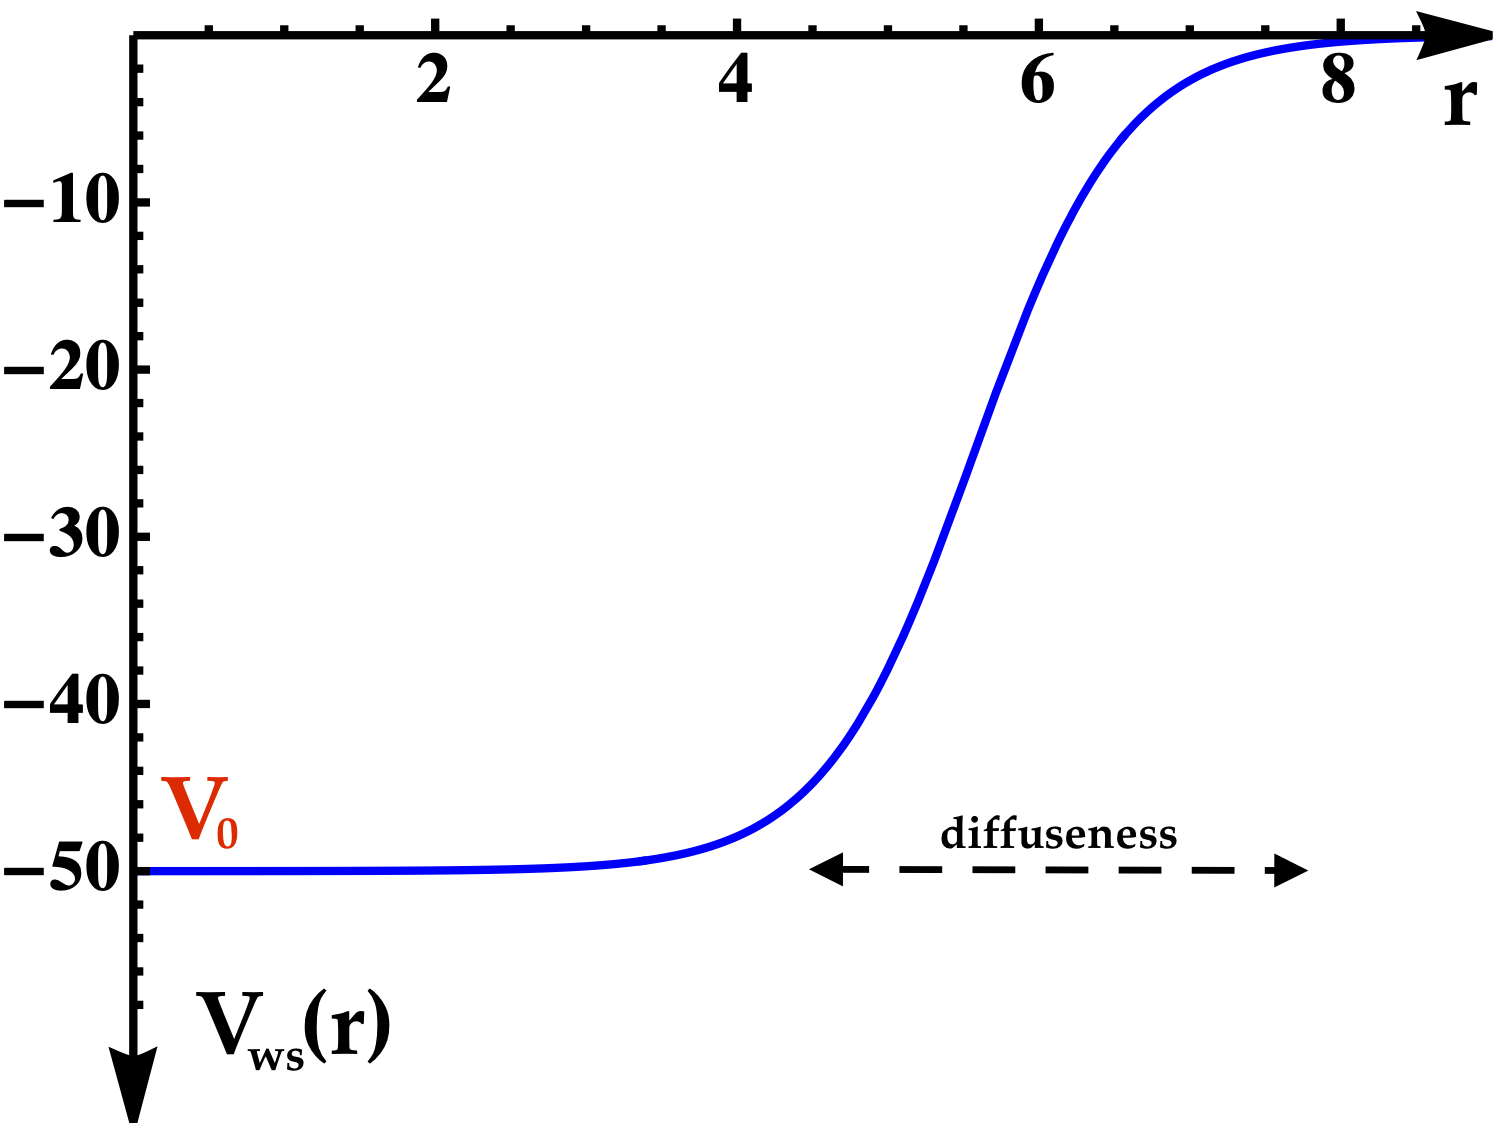
\includegraphics[scale=0.2]{Chapters/Figures/ws_potential_plot.png}
    \caption{The shape of the Woods-Saxon potential, defined by Eq. \ref{woods-saxon-potential}. The parameters are arbitrarily chosen as: $V_0=50$ MeV, $R=5.57$ fm, and $a=0.5$ fm.}
    \label{woods-saxon-plot}
\end{figure}

Fig. \ref{woods-saxon-plot} shows the shape of a typical Woods-Saxon potential. Aiming at a final Hamiltonian which describes the motion of the nucleon within the mean-field potential, the formula can be readily obtained:
\begin{align}
    H&=-\frac{\hbar^2}{2m}\nabla^2+V_\text{ws}^\text{central}+(\vec{l}\cdot\vec{s})_\text{term}\ ,\\
    H&=-\frac{\hbar^2}{2m}\nabla^2-\frac{V_0}{1+e^{\frac{r-R_0}{a}}}+A\vec{l}\cdot\vec{s}\ .
\end{align}
In addition to the shape of the Woods-Saxon potential, a comparison between it, a SHO,and the square-well-like potential is made in Fig \ref{shell-model-functional-potentials}.
\begin{figure}
    \centering
    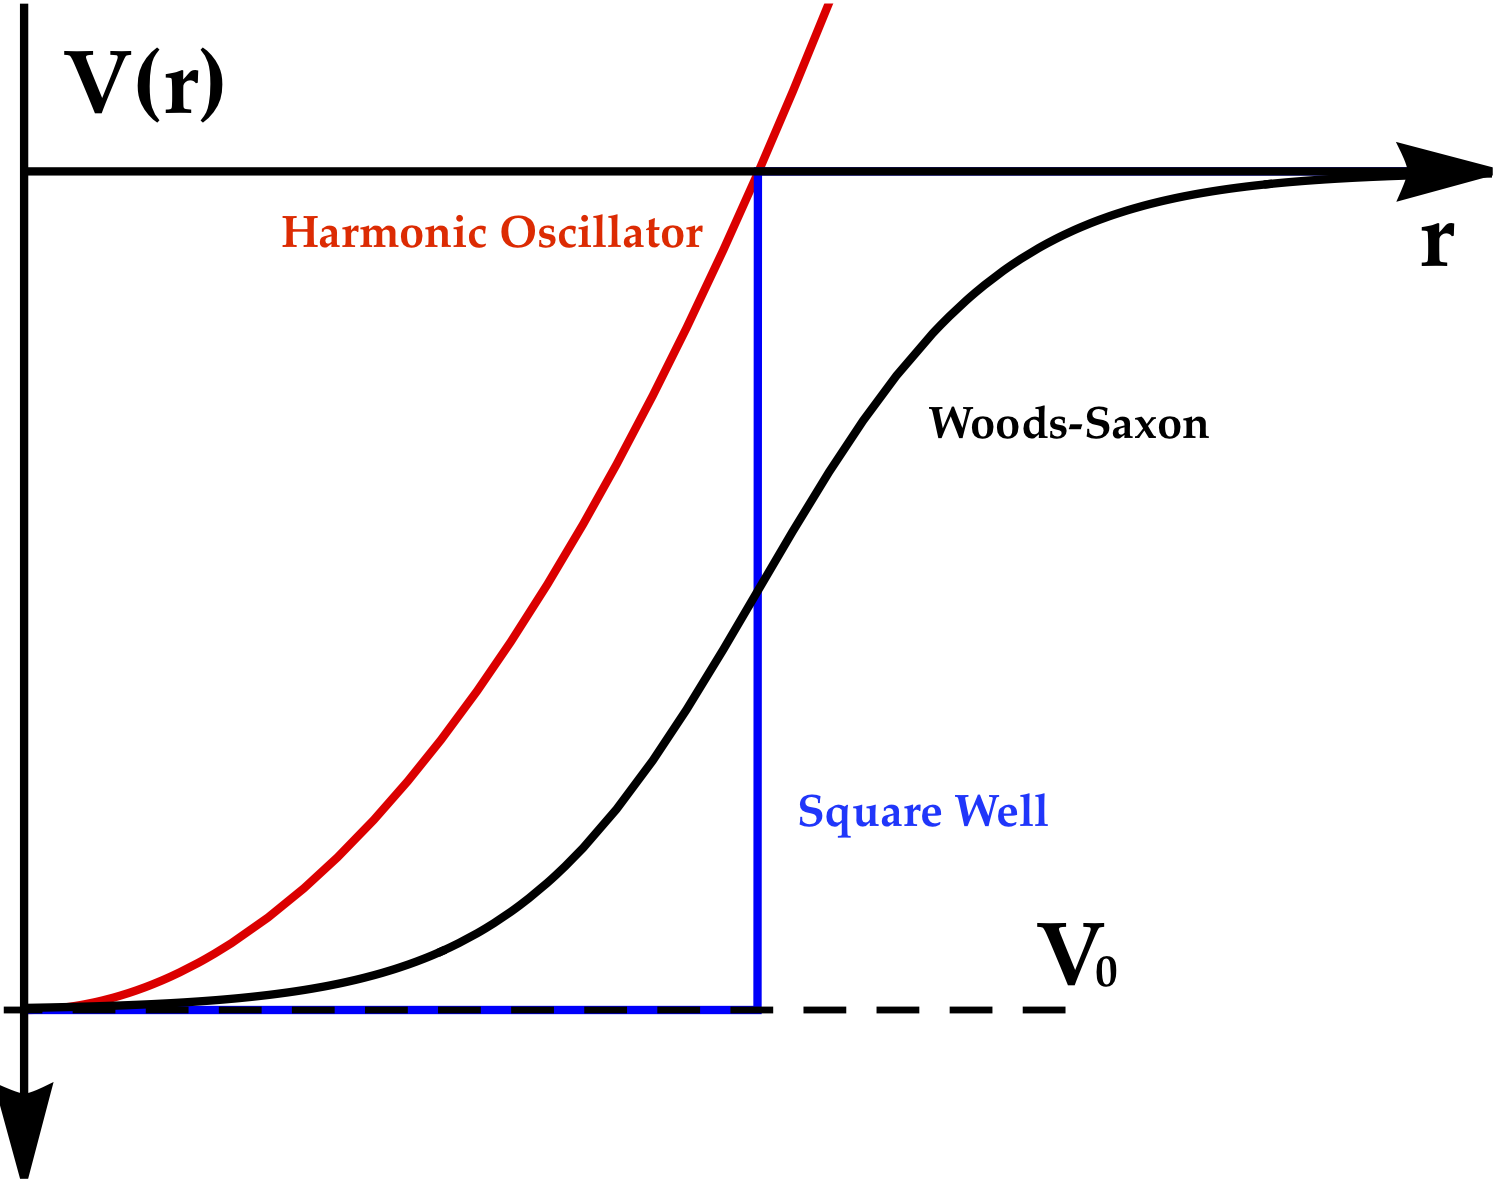
\includegraphics[scale=0.2]{Chapters/Figures/functional-potentials-shell-model.png}
    \caption{A schematic representation with the three kind of potentials used to describe the shell model: harmonic oscillator, Woods-Saxon, and for completeness, the square-well.}
    \label{shell-model-functional-potentials}
\end{figure}

The difference between the pure form of the Woods-Saxon potential and the total potential, where the spin-orbit contribution is amended, can be seen in Fig. \ref{woods-saxon-energy-levels}.
\begin{figure}
    \centering
    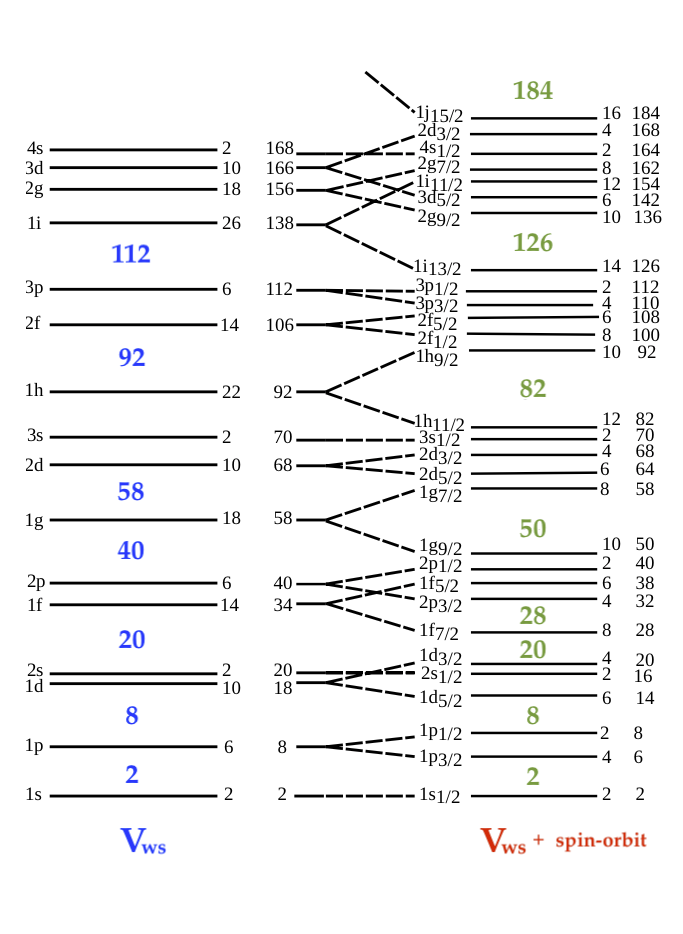
\includegraphics[scale=0.46]{Chapters/Figures/energy_levels_WS.png}
    \caption{The left side represents the energy levels calculated for the Woods-Saxon potential given by Eq. \ref{woods-saxon-potential}, and the right side shows the single-particle energies with the spin-orbit correction added, as in Eq. \ref{woods-saxon-so-potential}. Figure adapted from Ref. \cite{lewis2019lifetime}.}
    \label{woods-saxon-energy-levels}
\end{figure}

So far, the general discussion concerning the nuclear models was for the case where each nucleon is treated as an \emph{independent} particle moving in an average potential (mean-field potential) which represents an \emph{effective} interaction of all the other nucleons with the nucleon under study. However, such an assumption is not accurate enough (especially for the nuclei that lie far away from the closed shells), and this problem should be treated within a \emph{many-body} approach: considering the mutual interaction between the nucleons. These interactions are also called \emph{residual interactions} \cite{casten2000nuclear,bertulani2007nuclear}. With these residual interactions, an accurate depiction of the nucleus might be achieved, and in the following sections, the \emph{Deformed Shell Model} will be employed, reaching to the famous Nilsson model/theory of describing the nucleus.

\section{Deformed Shell Model}

In the previous section, the discussion was focused on an approximate description of the (independent) motion of a nucleon within an average potential. That potential is generated by the interaction of that nucleon with all the remaining nucleons within the compounding nucleus. Indeed, for spherical nuclei, the model described previously works really well and it is a successful tool in reproducing and predicting the properties of nuclear states, especially if the excited states have nucleonic configurations that are dominated by a single nucleon or a very small number of `extra' nucleons.

For nuclei that are even in both the proton number and the neutron number (i.e., even-even nuclei), the nuclear ground-state has a spin and parity that are properly reproduced by the \emph{spherical shell model}: $I^\pi=0^+$. In a nucleus with complete shells, the \emph{net spin} must be zero while for the nucleus with one nucleon missing from a complete shell closure (a hole), that ground-state spin should equal to the total a.m. $j$ value of the orbital which that particular hole is occupying. Moreover, the parity of the ground-state for a given nucleus is determined by the orbital a.m. value $l$:
\begin{align}\pi=(-)^l\to
    \begin{cases}
        +1 &\text{for even-}l\ \text{levels}\\
        -1 &\text{for odd-}l\ \text{levels}\\
   \end{cases}\ .
\end{align}
For odd-odd nuclei, one can find the ground-state (g.s.) spin and parity via the coupling of the spin and parity of the last two valence nucleons \cite{krane1991introductory,bertulani2007nuclear}. The coupling rules that are allowed in the odd-odd nucleus were determined more than 50 years ago by Gallagher et al. \cite{gallagher1958coupling}:
\begin{align}
    I&=j_p+j_n\ \text{if}\ j_p=l_p\pm\frac{1}{2}\ \text{and}\ j_n=l_n\pm\frac{1}{2}\ ,\\
    I&=|j_p-j_n|\ \text{if}\ j_p=l_p\pm\frac{1}{2}\ \text{and}\ j_n=l_n\mp\frac{1}{2}\ .
\end{align}

\subsection{Deformed Shell Model - Nilsson Model}

The idea that some nuclei are deformed in their ground-state was enforced experimentally a long time ago by measuring quantities such as density distributions, nuclear quadrupole moments \cite{casten2000nuclear} and so on. The non-spherical shapes are given by the existence of nucleonic configurations that lie away from the major shell closure. In Chapter \ref{chapter-2} the description of the nuclear shapes was treated, using the well-known formula for the parametrization of the nuclear radius in terms of the collective coordinates (see Eq. \ref{nuclear-shape}), resulting in the known nuclear shapes: \emph{spherical}, \emph{axially-symmetric} (that is prolate or oblate), and \emph{axially-asymmetric} (or triaxial). 

Developed by Nilsson in 1955 \cite{nilsson1955binding} for treating the \emph{deformed nuclei} proved to be a big pillar within the nuclear community, especially for the study of medium and heavy nuclei. In essence, this tools is a modified shell model which allows for deformations to be taken into account by the use of the \emph{anisotropic harmonic oscillator} (AHO). Similarly as for the basic shell model, the goal is to obtain an expression for the single-particle energies of a nucleon. The basic Hamiltonian corresponding to this kind of system is shown below \cite{bertulani2007nuclear}:
\begin{align}
    H=H_0+a_1\vec{l}\cdot\vec{s}+a_2l^2\ ,
    \label{nilsson-simple-hamiltonian}
\end{align}
where $H_0$ is a Hamiltonian for the AHO. The general expression for this kind of oscillator is of the form:
\begin{align}
    H_\text{AHO}\equiv H_0=-\frac{\hbar^2}{2m}\nabla^2+\frac{1}{2}m(\omega_x^2x^2+\omega_y^2y^2+\omega_z^2z^2)\ .
\end{align}
In the general expression of the single-particle Hamiltonian, the constants $a_1$ and $a_2$ are usually determined via adjustments to the experimental results. It can be seen that the centrifugal-like term $l^2$, which simulates a flattening of the oscillator potential, and the $\vec{l}\cdot\vec{s}$ term are still present here, as it was the case for the spherical shell model. However, the explicit form of Eq. \ref{nilsson-simple-hamiltonian} is as follows:
\begin{align}
    H_\text{Nil}=-\frac{\hbar^2}{2m}\nabla^2+&\frac{1}{2}m(\omega_x^2x^2+\omega_y^2y^2+\omega_z^2z^2)-2\kappa\hbar\omega_0(\vec{l}\cdot\vec{s})\nonumber\\&-2\kappa\hbar\omega_0\mu\left(l^2-\langle l^2\rangle_N\right)\ .
    \label{eq-full-nilsson-ham}
\end{align}
Obviously, the parameters $\kappa$ and $\mu$ act as strength parameters for the spin-orbit coupling term and the centrifugal term, respectively. The last term is a correction, which was originally considered as $\mu l^2$, but it was pointed by Gustafson et al. \cite{gustafson1967nuclear} that the shift in energy is way too large for big values of $N$ (principal quantum number). As a result, taking the current expression for the correction term helps to compensate. The three \emph{oscillator frequencies} are chosen to be inversely proportional to the semi-axis lengths of the deformed ellipsoid (denoted by $a_x$, $a_y$, and $a_z$) such that:
\begin{align}
    \omega_r=\omega_0\frac{R_0}{a_r}\ ,\ r=x,y,z\ .
\end{align}
For the spherical case, the oscillator frequency $\hbar\omega_0$ is set to $41A^{-1/3}$ MeV (calculation for this value arise from the shell model with SHO \cite{bertulani2007nuclear}). For the axially-symmetric case, one can choose the $z$-axis as symmetry axis, implying that thw oscillator frequencies along the $x$ and $y$ axes are equivalent (that is $\omega_x=\omega_y\equiv\omega_\perp$).

Following the calculations done in \cite{bertulani2007nuclear}, one can express the two relevant oscillator frequencies in terms of a deformation parameter $\epsilon_2$ (whose dependence on the quadrupole deformation parameter $\beta_2$ has been shown in Eq. \ref{epsilon-beta-relation}) as such:
\begin{align}
    \omega_\perp^2=\omega_0^2\left(1+\frac{2}{3}\epsilon_2\right)\ ,\\
    \omega_z^2=\omega_0^2\left(1-\frac{4}{3}\epsilon_2\right)\ .
    \label{oscillator-frequencies-nilsson}
\end{align}
Moreover, a dependence on the deformation parameter itself is employed for the frequency $\omega_0$ that appears in the expressions for $\omega_\perp$ and $\omega_z$, respectively:
\begin{align}
    \omega_0=\left(1-\frac{4}{3}\epsilon_2^2-\frac{16}{27}\epsilon_2^3\right)^{-1/6}\ ,
    \label{omega-0-oscillator-frequency}
\end{align}
where $\bar{\omega}_0$ can be considered a constant written as $\bar{\omega}_0=(\omega_x\omega_y\omega_z)^{1/3}=\text{const}$ (coming from the harmonic oscillator at zero deformation and also considering the conservation of the nuclear volume).

The energy eigenvalues $\epsilon_q$ for the nucleonic state $\psi_q$ belonging to a deformed nucleus can be determined within the Nilsson model by solving the Schrödinger equation associated to each nucleon in particular:
\begin{align}
    H_\text{Nil}\psi_q=\epsilon_q\psi_q\ ,
    \label{nilsson-schrodiner-equation}
\end{align}
where the index $q$ denotes a set with all the relevant quantum numbers. This set is also called the \emph{asymptotic quantum numbers}, and they are used to specify a \emph{Nilsson orbital}. The well-known notation is as follows (still considering the $z$-axis as the symmetry axis):
\begin{align}
    \Omega^\pi\left[Nn_z\Lambda\right]\ .
    \label{nilsson-notation}
\end{align}
\begin{itemize}
    \item $\Lambda$ is the projection of the particle's orbital a.m. along the symmetry axis (component of $l$ along $z$)
    \item $N$ the principal quantum number of the major shell. It also determines the parity as $\pi=(-1)^N$, making the notation from Eq. \ref{nilsson-notation} somewhat redundant in terms of explicitly specifying it
    \item $n_z$ is the number of oscillator quanta along the symmetry axis. More precisely, it gives the number of nodes for the wave-function of that particle along the direction of the $z$-axis
    \item $\Omega$ is the projection of the particle's total a.m. along the symmetry axis (i.e., $\mathbf{j}$). Moreover, the projection of the intrinsic spin of a nucleon onto the symmetry axis can have the values $\Sigma=\pm\frac{1}{2}$, so that $\Omega=\Lambda+\Sigma=\pm\frac{1}{2}$.
\end{itemize}

Fig. \ref{fig-nilsson-quantum-numbers} shows the geometrical meaning of the asymptotic quantum numbers for the Nilsson model. Indeed, for a single nucleon orbiting a deformed core, the vector $\mathbf{R}$ represents the angular momentum of a \emph{rotating nucleus} (having a collective character, since it emphasizes the motion of the nucleus as a whole), the vector $\mathbf{I}$ represents the total a.m. of the entire nucleus, $\mathbf{j}$ is the total a.m. of the single-particle (that is $\mathbf{j}=\mathbf{j}+\mathbf{s}$). However, two more quantum numbers should be mentioned: the projection of the total a.m. $\mathbf{I}$ onto the symmetry axis, denoted by $K$, and the projection of the same vector onto the laboratory axis, referred to as $M$.

\begin{figure}
    \centering
    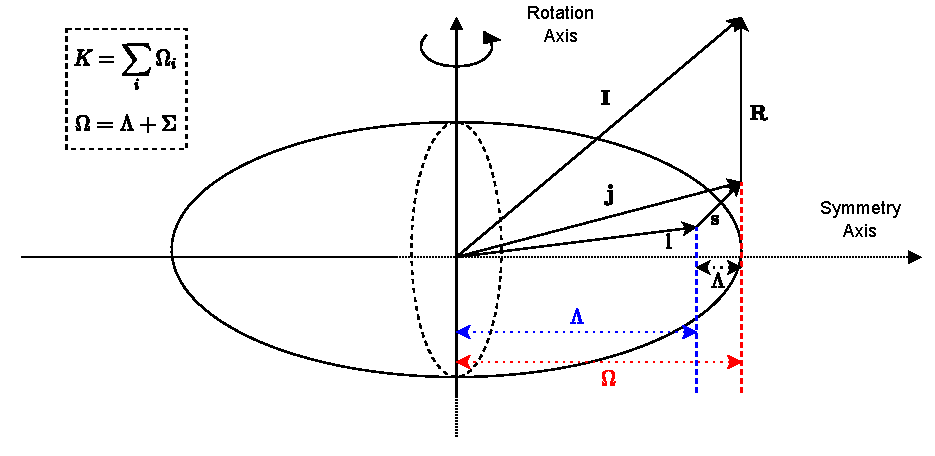
\includegraphics[scale=1]{Chapters/Figures/nilsson_quantum_numbers.pdf}
    \caption{A schematic drawing that shows the geometrical interpretation of the Nilsson asymptotic quantum numbers (see text). This figure is inspired from Ref. \cite{garnsworthy2007neutron}}
    \label{fig-nilsson-quantum-numbers}
\end{figure}

Regarding the quantum numbers sketched in Fig. \ref{fig-nilsson-quantum-numbers}, there is an important aspect which needs to be specified about the two projections $K$ and $\Omega$, respectively, since it would make the understanding of the orbital motion of nucleons more concise. Indeed, it is clear that compared to the spherical case, where different orientations are irrelevant to the energy spectrum of nucleons, here in the deformed case, different directions in space lead to different energies. The orientation is in fact specified by the \emph{magnetic sub-state} of the nucleon, i.e., the projection of the total angular momentum on the symmetry axis. This projections is denoted by $\Omega$ for the single-particle, however, because the rotational angular momentum $\mathbf{R}$ in the axially deformed is perpendicular to the symmetry axis for low-lying states, then it will have no contribution to $K$, meaning that one can use $\Omega$ and $K$ interchangeably.

\subsection{Single-particle states in deformed nuclei}

It is instructive to go into detail about the quantum numbers defined in Eq. \ref{nilsson-notation} since the orbits which characterize the nucleons with such numbers help to point out the nature of nuclear deformations that take place.

The quantum numbers $N$, $n_z$ and $\Lambda$ are good quantum numbers only when the nuclear deformation is large, meaning that $\epsilon$ (or equivalently $\beta$) tends to infinity: also the reason why they are called asymptotic quantum numbers. However, the numbers $\Omega$ and $\pi$ remain good quantum numbers even for low and moderate deformations for the nucleus. It should be noted that if $N$ is even, then $(\Lambda+n_z)$ is also even. Similarly, if $N$ is odd, then the sum of the other two quantum numbers must also be odd \cite{casten2000nuclear}.

Since the eigenvalues of the Hamiltonian $H_\text{Nil}$ ultimately depend on the deformation parameter $\epsilon$, each nucleon will have an orbit (energy) that is deformation dependent. At no deformation (i.e., the spherical case), all the energy levels for a single-particle state will have a $2j+1$ degeneracy. This translates to the fact that all $2j+1$ possible orientations of $\vec{j}$ are equivalent, when referring to any arbitrary axis of choice. On the other side, when the potential is deformed, this will no longer hold: the energy levels in the deformed potential will depend on the spatial orientation of the orbit itself: the energy depends on the component of $\vec{j}$ along the symmetry axis of the core. 

As an example, a nucleon from the $f_{7/2}$ shell will be considered. This nucleon can have eight possible components for $\vec{j}$, this is the range $\Omega=[-\frac{7}{2},\frac{7}{2}]$. Because of the reflection symmetry for nuclei for either of the two possible directions of the symmetry axis, the positive components of $\Omega$ will have the same energy as the negative ones: leading to a degeneracy of the levels. Now, the single-particle $f_{7/2}$ state will split up into four new states when deformation emerges: $\Omega=\frac{1}{2},\frac{3}{2},\frac{5}{2},\frac{7}{2}$ and all have negative parity. In Fig. \ref{nillson-orbits-prolate-projections} an illustration with the different orbits of the odd particle is given, for both the prolate deformed nuclei as well as for oblate ones. Similarly, the orbits of the same state are pictorially represented in Fig. \ref{nillson-orbits-oblate-projections}.

\begin{figure}
    \centering
    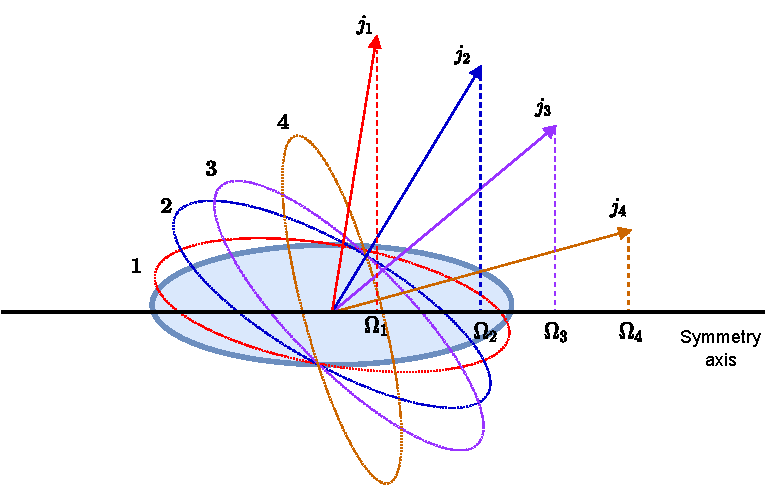
\includegraphics[scale=1]{Chapters/Figures/nillson_SP_orbits.pdf}
    \caption{A simple sketch showing the single-particle orbits for the $j=7/2$ nucleonic state, along the symmetry axis for a \emph{prolate} deformation. The actual projections are $\Omega_1=\frac{1}{2}$, $\Omega_2=\frac{3}{2}$, $\Omega_3=\frac{5}{2}$, and $\Omega_4=\frac{7}{2}$. The figure was inspired from Ref. \cite{krane1991introductory}.}
    \label{nillson-orbits-prolate-projections}
\end{figure}

\begin{figure}
    \centering
    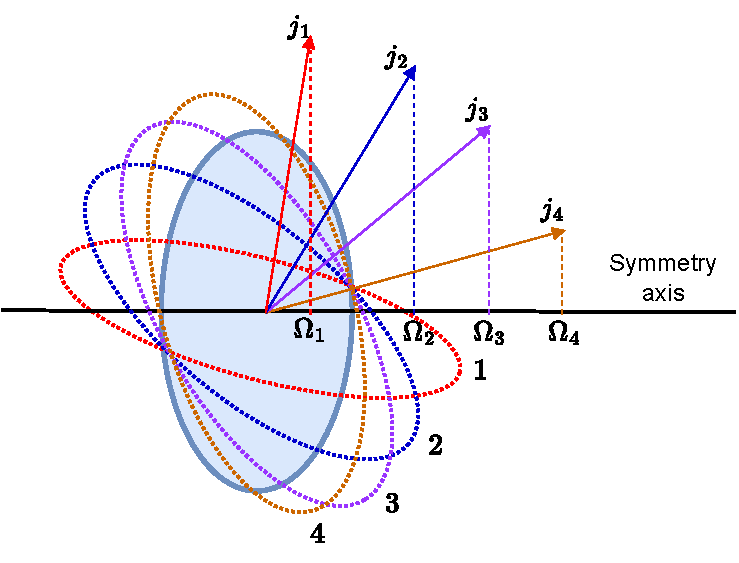
\includegraphics[scale=1]{Chapters/Figures/nillson_SP_orbits_2.pdf}
    \caption{A simple sketch showing the single-particle orbits for the $j=7/2$ nucleonic state, along the symmetry axis for a \emph{oblate} deformation. The actual projections are $\Omega_1=\frac{1}{2}$, $\Omega_2=\frac{3}{2}$, $\Omega_3=\frac{5}{2}$, and $\Omega_4=\frac{7}{2}$. The figure was inspired from Ref. \cite{krane1991introductory}.}
    \label{nillson-orbits-oblate-projections}
\end{figure}

From Figs. \ref{nillson-orbits-prolate-projections} - \ref{nillson-orbits-oblate-projections}, it can be seen that the first orbit (denoted by orbit $1$) lies closest to the core in the prolate case, while in the oblate case this is true for orbit $4$. This plays the role in the interaction strength, meaning that for the prolate case, the orbit $1$ will interact the strongest with the \emph{core}, while in the oblate case, it is the orbit $4$ which has the strongest interaction with the bulk core. Moreover, the strength of interaction indicates the magnitude of the energies for each projection: the stronger the interaction between the orbit and the core, the more tightly bound these states are and lie lower in energy. For prolate deformations, the orbits with smallest $\Omega$ `prefer' to lie lower in energy (interacting strongly with the core). For oblate deformations, the situation is opposite: orbits with the maximal $\Omega$ have the strongest core interactions and therefore lie lowest in energy.

Another way of looking at the coupling of the single-particle with the bulk core can be given in terms of overlaps of their corresponding wave-functions (eigenstates). Indeed, a nucleon lying in the lowest $\Omega$ orbit will have a \emph{maximum} wave-function overlap with a prolate core. On the other hand, nucleons lying in the highest $\Omega$ orbits will have maximum overlap of the wave-function with an oblate core. The overlap gives the overall binding energy between the two systems (i.e., core and particle) as explained in the previous paragraph. Discussion about the wave-function overlap and the nuclear density distribution \cite{frauendorf2014transverse, das2018nuclear} will be made in the following chapters.

The induced degeneracy due to deformation for a particle state $l_j$ is shown in Fig. \ref{nillson-orbits-splittings}, for the same example of the nucleon with the orbit $f_{7/2}$.

\begin{figure}
    \centering
    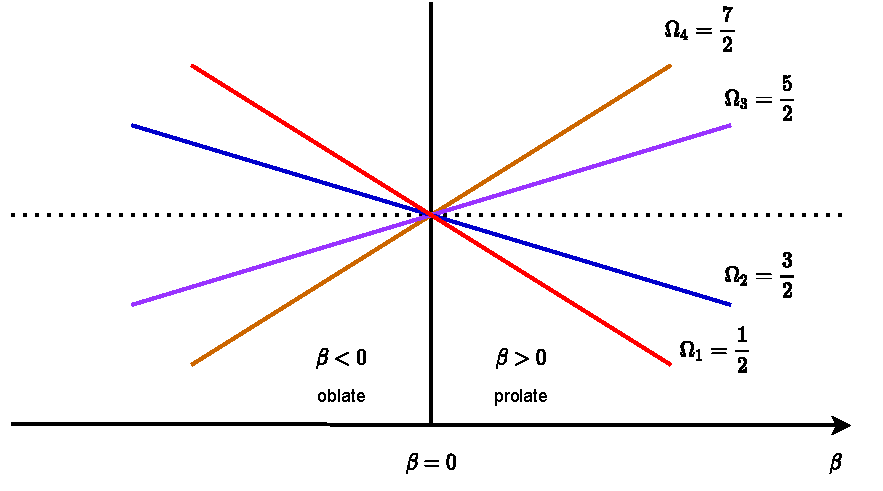
\includegraphics[scale=0.95]{Chapters/Figures/nillson_SP_splittings.pdf}
    \caption{The effect of deformation for the particle state $f_{7/2}$. It can be seen that indeed, as it was mentioned within the text, $\Omega_1$ component lies lowest in energy for the oblate deformation, and $\Omega_4$ component lies the lowest in energy for an oblate deformation.}
    \label{nillson-orbits-splittings}
\end{figure}

Obviously, the sketch shown in Fig. \ref{nillson-orbits-splittings} is just an instructive example, and it does not represent an accurate description of the single-particle energies for deformed nuclei. In fact, if the potential is deformed, the quantum numbers $l$ and $j$ are not valid anymore (that is, the angular momentum is no longer a constant of motion for non-spherical potentials). A proper description of the single-particle orbits are represented by the so-called \emph{Nilsson diagrams}, where the energy for each state is represented as a function of the deformation parameter. Remember that the energies are in fact the eigenvalues of the Schrödinger equation associated to the initial Nilsson deformed Hamiltonian (see Eq. \ref{nilsson-schrodiner-equation}).

The spectrum of one-particle orbits plays an invaluable role within the nuclear structure and the study of deformed nuclei: the picture of one-particle motion in deformed potential works for deformed nuclei much better than the case of single-particle motion in spherical potentials for spherically shaped nuclei. Multiple quantitative analyses have been performed on experimental data of well-deformed (especially odd-$A$) nuclei, from light ($^{25}$Mg, $^{25}$Al) to heavy ($^{169}$Tm, $^{175}$Yb, $^{177}$Yb) \cite{hamamoto2016interplay}. Examples with this kind of diagrams are shown in Figs. \ref{nillson-diagram} - \ref{nillson-diagram-2}. 

\begin{figure}
    \centering
    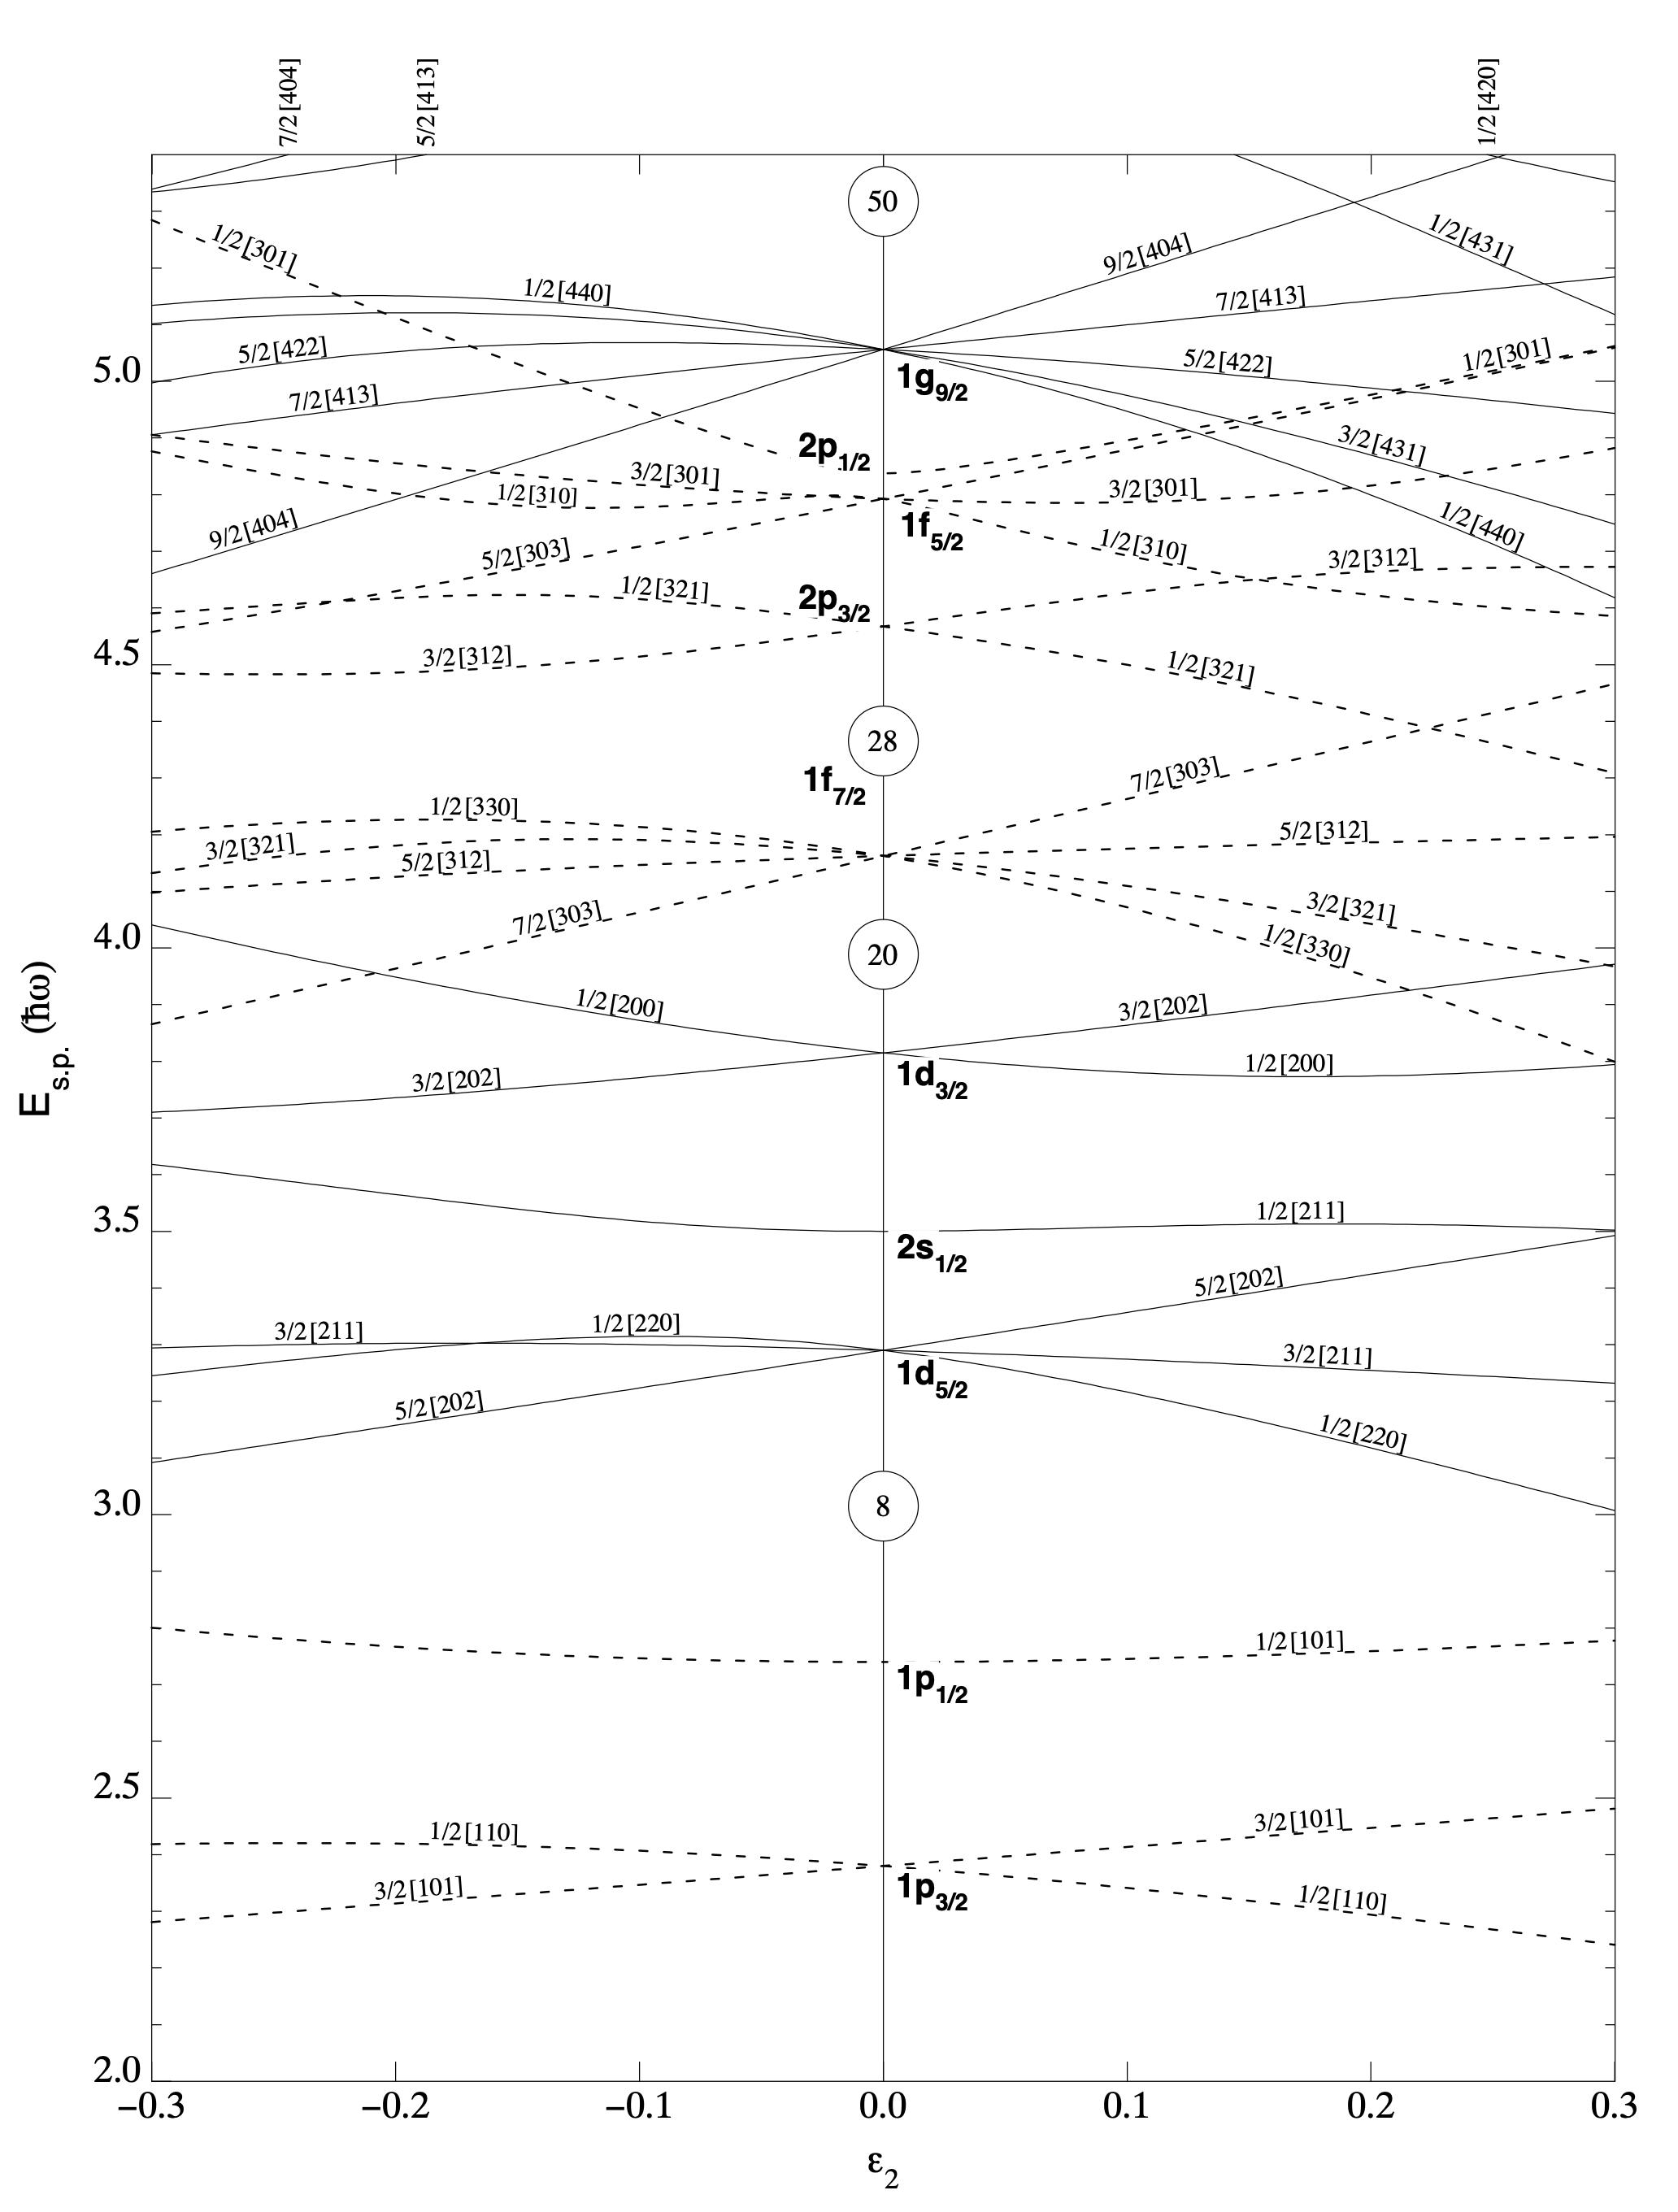
\includegraphics[scale=0.185]{Chapters/Figures/nillson_diagram.png}
    \caption{A Nilsson diagram for protons or neutrons, with $Z$ or $N\leq50$. Picture reproduced from Ref. \cite{ragnarsson2005shapes}.}
    \label{nillson-diagram}
\end{figure}

\begin{figure}
    \centering
    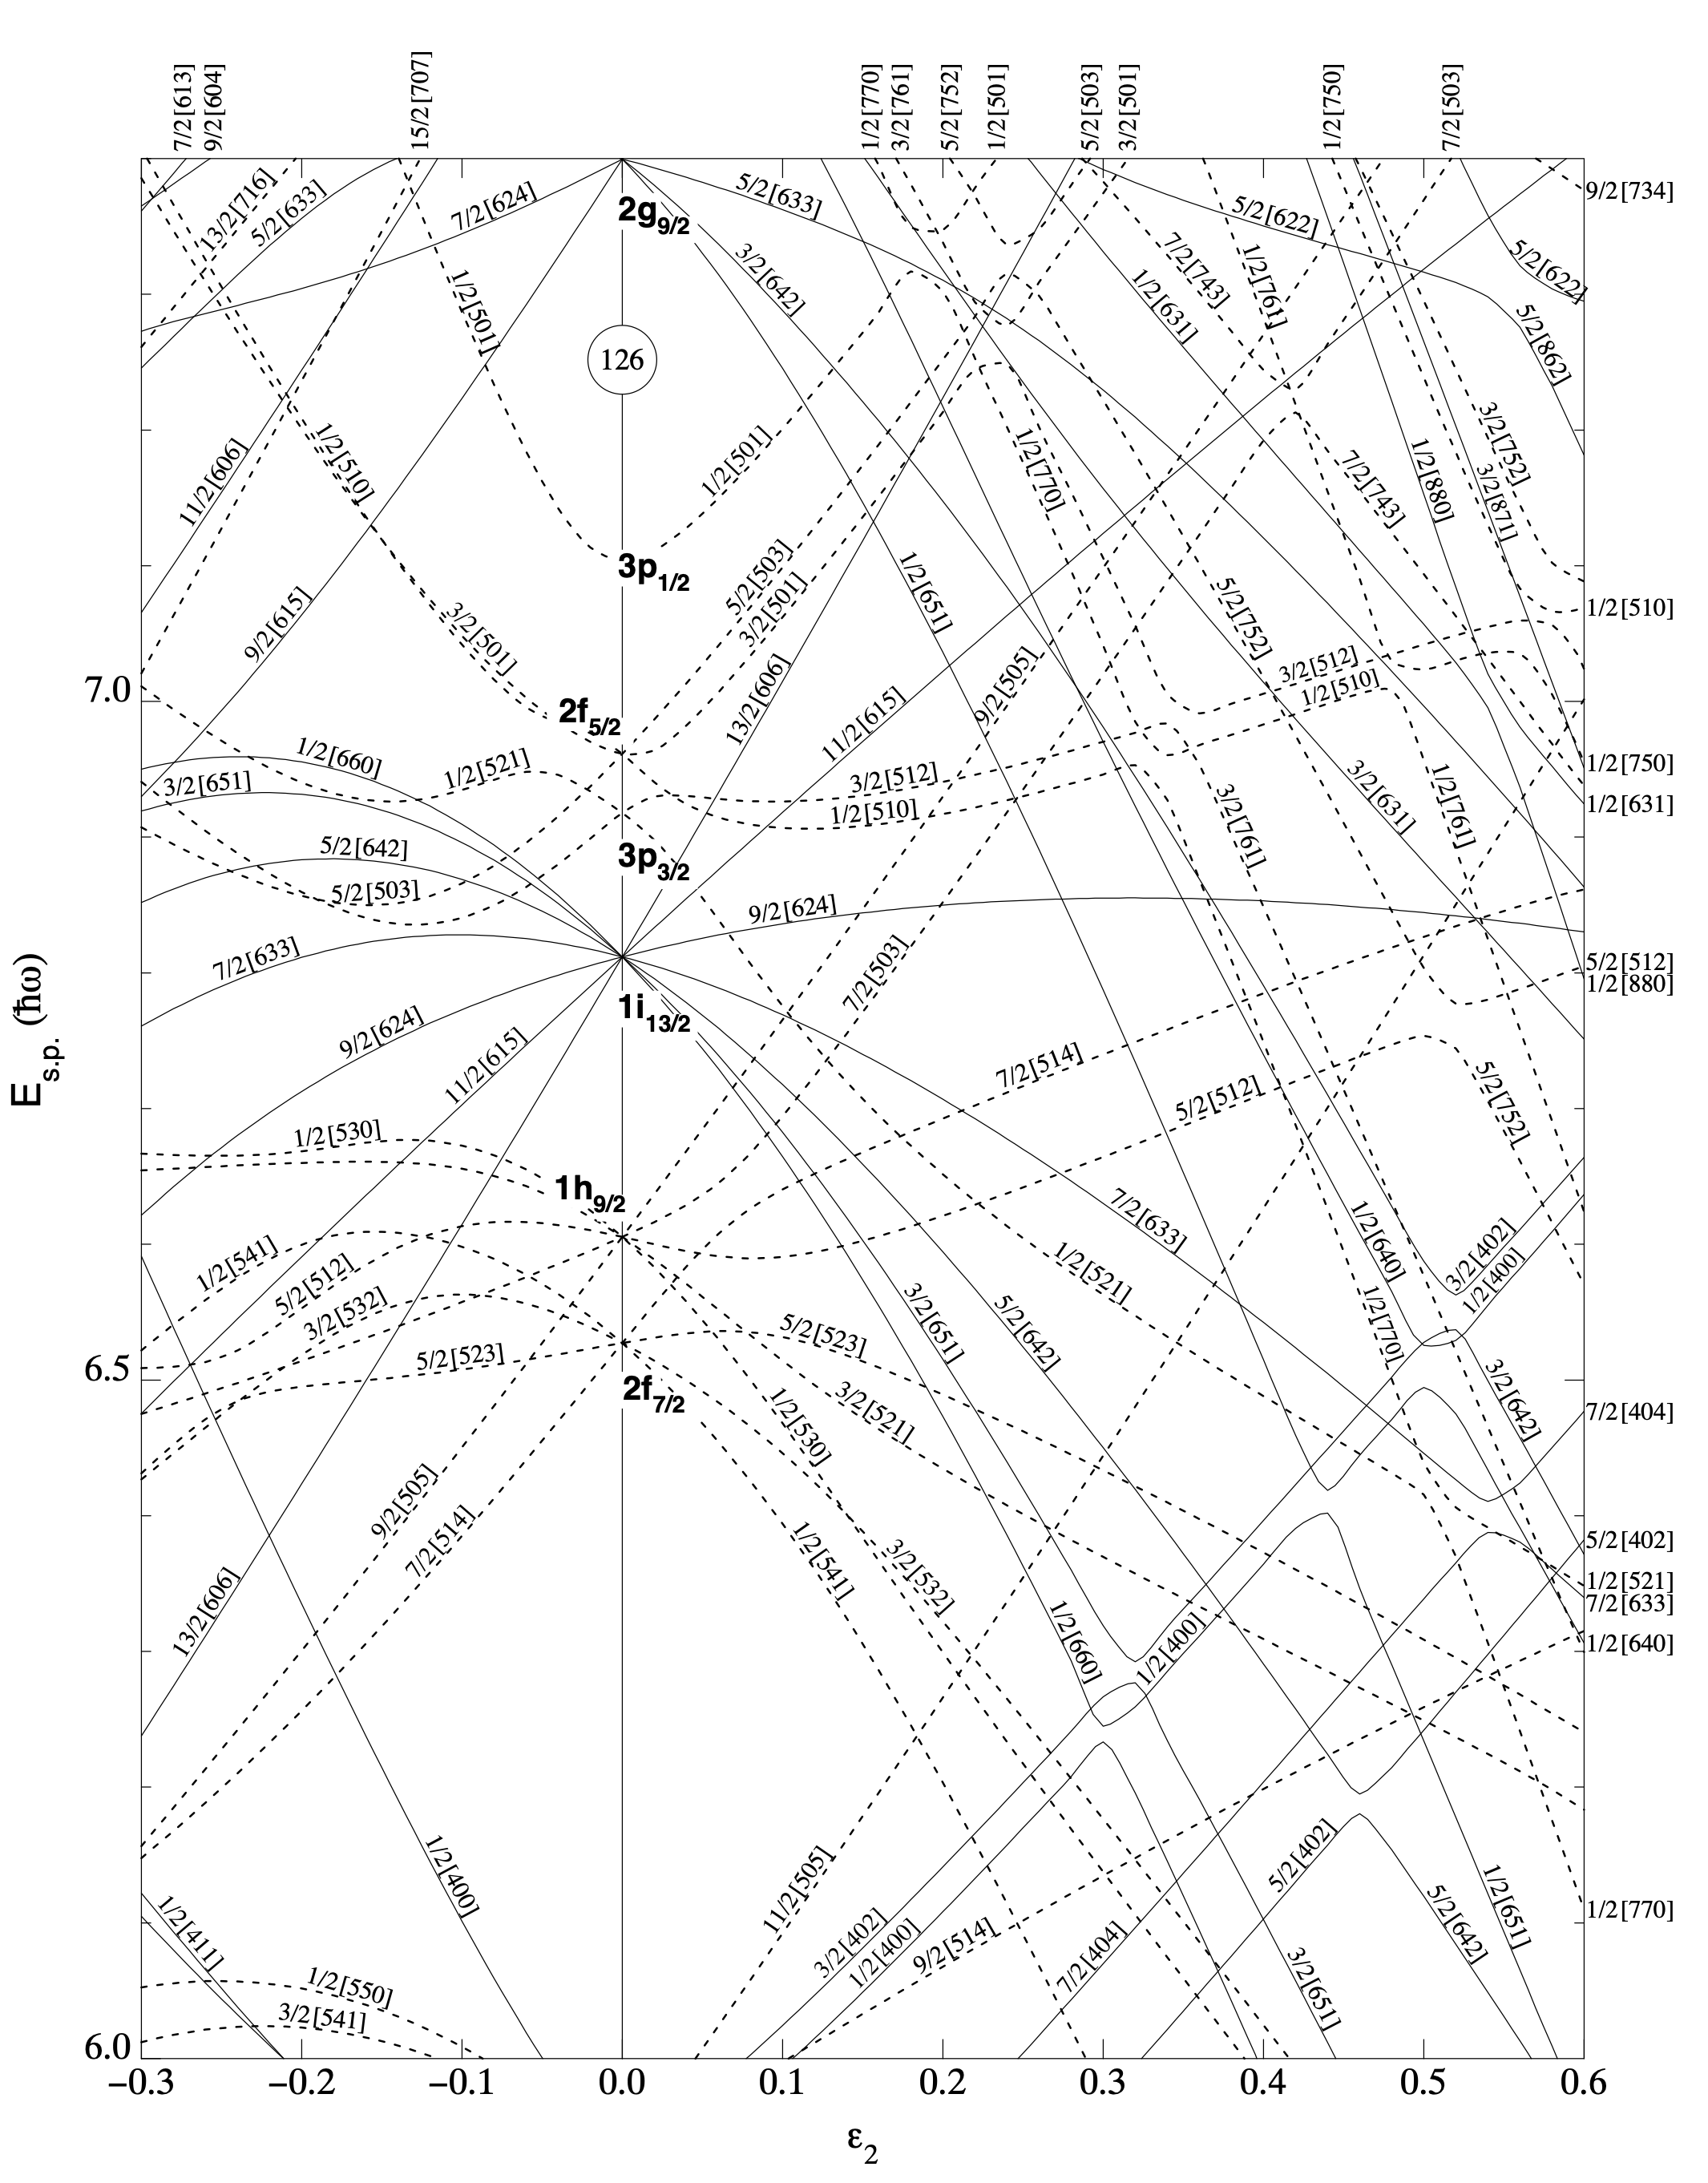
\includegraphics[scale=0.185]{Chapters/Figures/nillson_diagram_2.png}
    \caption{A Nilsson diagram for neutrons, with $82\leq N\leq126$. %This diagram also shows the orbits of neutrons from nuclei such as the Lu isotopes which will be studied in this work.
    Picture reproduced from Ref. \cite{ragnarsson2005shapes}.}
    \label{nillson-diagram-2}
\end{figure}

It can be seen that each state within a Nilsson diagram is represented as a solid line or a dashed line, depending on its parity (remember that the parity quantum number is given by $(-1)^N$ or, equivalently, by $(-1)^l$). The labelling from the Figs. \ref{nillson-diagram} - \ref{nillson-diagram-2} is consistent with the one defined in the previous subsection.

Another important aspect which can be seen in the Nilsson diagrams (for some orbits) is the `crossing' between states with different quantum numbers. In order to fully understand this concept, it is instructive to go into detail about \emph{two-state mixing}.

\subsubsection*{Two-state mixing}

In the work of Casten \cite{casten2000nuclear}, an analytical approach is given for treating the mixing of two different states (energy levels). It starts from the basic idea of two initial levels, each with its corresponding energy $E_1$ and $E_2$, and their associated wave-functions (denoted here with $\psi_1$ and $\psi_2$). Any interaction between them results in the mixing matrix element $\bra{\psi_1}V_\text{int}\ket{\psi_2}$, where $V_\text{int}$ is the arbitrary interaction between the states. This is sketched in Fig. \ref{two-state-mixing-scheme}.

\begin{figure}
    \centering
    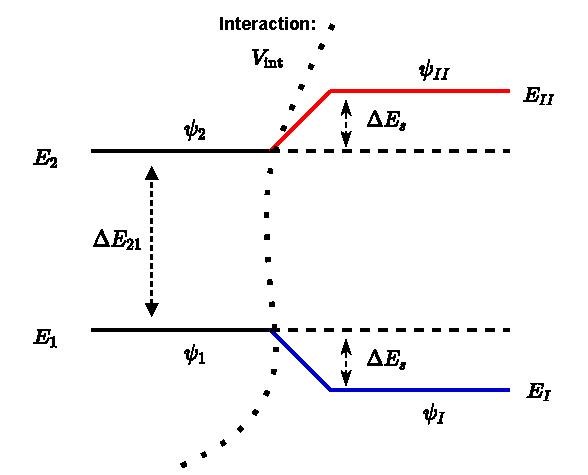
\includegraphics[scale=0.95]{Chapters/Figures/two-state-mixing.pdf}
    \caption{Defining the mixing between two different states, with two corresponding energies and wave-functions. Interaction is illustrated via the curved line and $V_\text{int}$ term.}
    \label{two-state-mixing-scheme}
\end{figure}

This problem can be solved by finding the final energies and wave-functions, this being done via the diagonalization procedure of a $2\times 2$ matrix, where the main diagonal contains the two energies and off-diagonal terms represent the interaction itself. The final states will be denoted here with ($E_I$, $E_{II}$) for the energies and ($\psi_I$, $\psi_{II}$) for the wave-functions. As a general rule, the mixing depends on the initial separation $\Delta E_{21}=(E_2-E_1)$ and the matrix element $\bra{\psi_1}V_\text{int}\ket{\psi_2}$. Given a large spacing, the effect of a given matrix element will be quenched. Moreover, even for a small matrix element, it can introduce a large mixing if the energy separation between the states is small (that is, the unperturbed states are lie close in energy). 

A reduction from these two parameters can be performed, obtaining a single universal mixing expression that is valid for any arbitrary interaction and any initial spacing. As a first step, one should define the ratio between the spacing of the unperturbed states ($Delta E_{21}$) and the strength of the matrix element:
\begin{align}
    R=\frac{\Delta E_{21}}{V_\text{int}}\ .
\end{align}
With this quantity, the newly perturbed energies $E_I$ and $E_{II}$ are readily obtained \cite{casten2000nuclear}:
\begin{align}
    E_I&=\frac{1}{2}(E_1+E_2)+\frac{\Delta E_{21}}{2}\sqrt{1+\frac{4V_\text{int}^2}{\Delta E_{21}^2}}\ ,\\
    E_{II}&=\frac{1}{2}(E_1+E_2)-\frac{\Delta E_{21}}{2}\sqrt{1+\frac{4V_\text{int}^2}{\Delta E_{21}^2}}\ .
    \label{eq-two-state-mixing-energies}
\end{align}

Even more useful would be to find the amount by which each energy is shifted after the interaction. This is denoted in Fig. \ref{two-state-mixing-scheme} by $\Delta E_S$ and its expression depends on $\Delta E_{12}$ as such:
\begin{align}
    |\Delta E_S|=|E_{II}-E_2|=|E_{I}-E_1|=\frac{\Delta E_{21}}{2}\left[\sqrt{1+\frac{4}{R^2}}-1\right]\ .
    \label{eq-shift-mixed-states}
\end{align}
The two perturbed wave functions are as follow:
\begin{align}
    \psi_I&=\alpha\psi_1+\beta\psi_2\ ,\nonumber\\
    \psi_{II}&=-\beta\psi_1+\alpha\psi_2\ ,
\end{align}
where the two amplitudes $\alpha$ and $\beta$ must verify the condition $\alpha^2+\beta^2=1$ and:
\begin{align}
    \beta=\frac{1}{\left\{1+\left[\frac{R}{2}+\sqrt{\frac{R^2}{4}+1}\right]^2\right\}^{1/2}}
    \label{eq-beta-mixing-amplitude}
\end{align}

It is noteworthy to point out that the amplitude $\beta$ is in fact a function that only depends on $R$ (i.e., the ratio between the unperturbed energy splitting and the interaction strength). Similarly, by dividing the shift in energy $\Delta E_S$ to the initial splitting $\Delta E_{21}$, one will obtain an expression that is independent of the initial level spacing:
\begin{align}
    \frac{|\Delta E_S|}{\Delta E_{21}}=\frac{|E_{II}-E_{2}|}{\Delta E_{21}}=\frac{|E_{I}-E_{1}|}{\Delta E_{21}}=\frac{1}{2}\left[\sqrt{1+\frac{4}{R^2}}-1\right]
\end{align}

The importance of these formula will be now emphasized through a numerical example. First of all, the evolution of the ratio of the unperturbed shift and the interaction can be graphically represented as a function of the small mixing amplitude $\beta$ by the use of Eq. \ref{eq-beta-mixing-amplitude}. The graphical representation is shown in Fig. \ref{fig-beta-mixing-amplitude}. Following this analysis, also in Fig. \ref{fig-beta-mixing-amplitude} the shape of $R$ as a function of the energy shift of the perturbed states can be visualized.

\begin{figure}
    \centering
    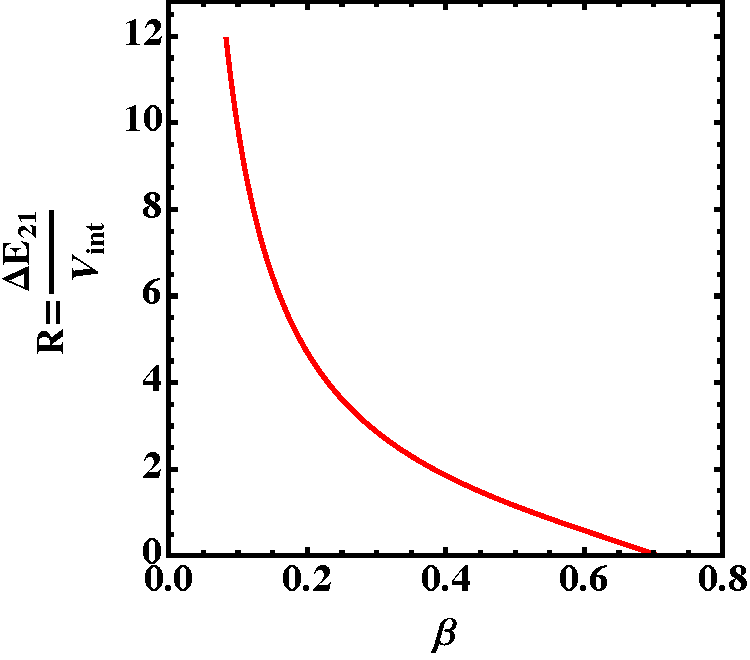
\includegraphics[scale=0.5]{Chapters/Figures/beta_mixing_amplitude.pdf}
    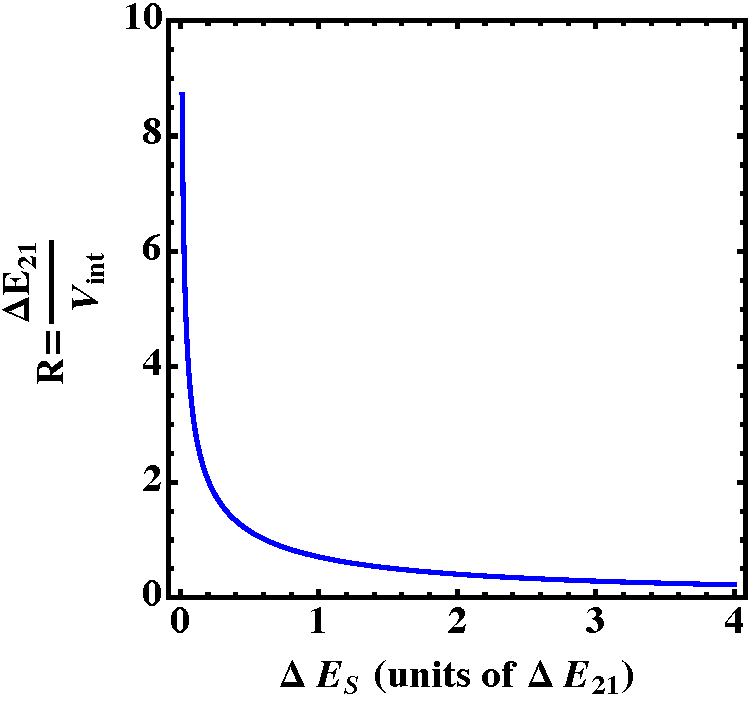
\includegraphics[scale=0.5]{Chapters/Figures/energy_shift_mixing_shape.pdf}
    \caption{\textbf{Left:} The dependence of $R$ (see text) on the mixing amplitude $\beta$. \textbf{Right}: The dependence of $R$ (see text) on the energy shift of the perturbed states ($\Delta E_S$).}
    \label{fig-beta-mixing-amplitude}
\end{figure}

For an arbitrary case where two initial states are separated by, say $\Delta_{21}=0.07$ MeV, and they become \emph{perturbed} via the interaction with a strength $V_\text{int}=0.03$ MeV, this gives a value of $R=3.5$ and, moreover, the mixing amplitude is $beta=0.256$. The two states will both be shifted by only $\Delta E_S=5.31$ keV (accounting for about $7.6 \%$ of the initial separation). Indeed, for this particular example, the perturbation results in an energy shift that is rather small compared to the initial state spacing.

% \begin{figure}
%     \centering
%     \caption{}
%     \label{mixing-energy-shift-shape}
% \end{figure}

Besides the numerical example discussed above, there are also two extremely important limiting situations when two states interact via a perturbation. The first one is the so-called \emph{strong mixing limit}, when the two initial states are degenerate (i.e., there is practically no spacing between them and $\Delta_{21}=0$). In this situation, the analytical expressions from Eq. \ref{eq-shift-mixed-states} fail to provide a quantitative analysis, but from Eq. \ref{eq-two-state-mixing-energies} a small adjustment of the expression will give rise to the following:
\begin{align}
    E_{I,II}=\frac{1}{2}\left[(E_1+E_2)\pm2V_\text{int}\right]=E_0\pm V_\text{int}\ ,
\end{align}
where the initial (common) energy of the two degenerate states is denoted by $E_0$. The above equation indicates the important fact that the energy shift which the two states suffer via the perturbation is only given by the \emph{mixing matrix element}. This means that the final separation energy for a two-state isolated system can never be closer than twice the interaction strength ($2V$). In the degeneracy case, the values for $\beta$ and $\alpha$ are readily obtained: ($\beta=\alpha=\frac{1}{\sqrt{2}}=0.707$), such that the states are completely mixed. Consequently, the mixed wave-functions of two (initially) degenerate states do not depend on the strength $V_\text{int}$ between them. The limiting case of \emph{strong mixing} of two degenerate levels is sketched in Fig. \ref{strong-mixing-fig}.

\begin{figure}
    \centering
    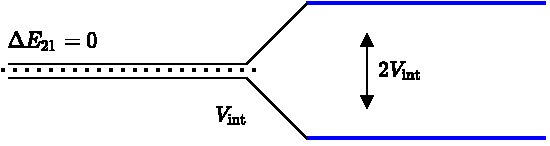
\includegraphics[scale=0.95]{Chapters/Figures/mixing_strong_coupling.pdf}
    \caption{The \emph{strong mixing} limit for two energy levels that are interacting via a perturbation. The initial two levels are degenerate, such that their splitting is null.}
    \label{strong-mixing-fig}
\end{figure}

The second limiting case is called \emph{weak mixing limit}, corresponding to a very large value of $R$ (meaning that the initial separation of the states is very large compared to the magnitude of the interaction itself). The shift in energy of the perturbed states in this case is given by:
\begin{align}
    \frac{|\Delta E_S|}{\Delta E_{21}}=\frac{1}{R^2}\ .
\end{align}

A graphical representation for the weak mixing is shown in Fig. \ref{weak-mixing-fig}.

\begin{figure}
    \centering
    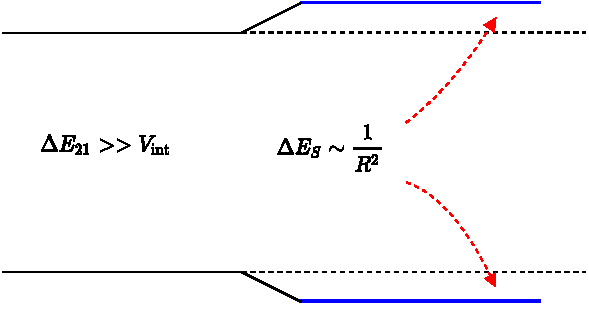
\includegraphics[scale=0.95]{Chapters/Figures/mixing_weak_coupling.pdf}
    \caption{The \emph{weak mixing} limit for two energy levels that are interacting via a perturbation. The interaction strength is much smaller than the initial spacing between states, resulting in a very small energy splitting $\Delta E_{S}$.}
    \label{weak-mixing-fig}
\end{figure}

As a final step in the analysis of the two-state mixing, it is worth mentioning a corner-case which will help to get a better grasp of the Nilsson orbitals. Consider two states (say $\psi_1$ and $\psi_2$) whose energies are parametrized in terms of some argument $c_\text{nuc}$ which is relevant for the nuclear structure of that system (e.g., $c_\text{nuc}$ could be a quadrupole deformation and the two initial states are in fact Nilsson orbits). The remarking `feature' of this hypothesis is that if there indeed exists mixing between the two states, they can never cross each other. The two mixed states will always repel and they can never be closer than twice the mixing matrix element $V_\text{int}$ after mixing occurs. In Fig. the behavior of non-crossing for the mixed states is sketched.
The point at which the two states are the closest to each other represents the case when the wave-functions contain similar admixtures of each of the initial states (unperturbed). The \emph{inflection point} can be seen in Fig. \ref{fig-non-crossing}, where the behavior of the final states $\psi_I$ and $\psi_{II}$ can be seen.

\begin{figure}
    \centering
    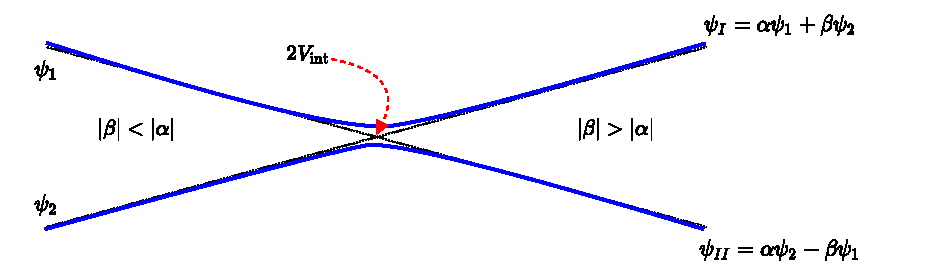
\includegraphics[scale=0.9]{Chapters/Figures/state_non_crossing.pdf}
    \caption{A sketch showing the concept of \emph{non-crossing} between two states. Arrow represents the closest point at which the two states can interaction with each other (i.e., the inflection point).}
    \label{fig-non-crossing}
\end{figure}

\subsection*{Nilsson orbitals}

With the concept of two-state mixing clearly depicted, it is instructive to go further into the Nilsson orbitals and their significance. Recalling Fig. \ref{nillson-orbits-splittings}, the splitting of a $j$ orbital into $j+1/2$ magnetic sub-states can be viewed as a set of orbitals (energies) where the nucleon orbits around the bulk nucleus with an orbit that has a certain \emph{tilt} angle $\theta$ (see the orbits depicted in Figs. \ref{nillson-orbits-prolate-projections} and \ref{nillson-orbits-prolate-projections}). The tilting angle is conceptually showed in Fig. \ref{fig-nilsson-tilting-angle}, where a magnetic sub-state with given $\Omega$ is shown. For that particular orbit, the angle is given by the expression \cite{krane1991introductory,casten2000nuclear}:
\begin{align}
    \sin\theta&=\frac{\Omega}{j}\ , \nonumber\\
    \theta&=\arcsin(\frac{\Omega}{j})\ .
\end{align}
\begin{figure}
    \centering
    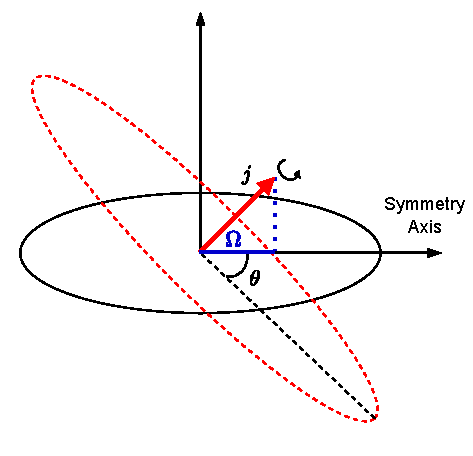
\includegraphics[scale=0.95]{Chapters/Figures/nilsson_tilting_angle.pdf}
    \caption{The orbit of a single particle orbiting the deformed nucleus, defined by the projection of the particle's a.m. $\Omega$ (on the symmetry axis) and the tilting angle $\theta$. Figure inspired from Ref. \cite{casten2000nuclear}}
    \label{fig-nilsson-tilting-angle}
\end{figure}

The change of $\theta$ is rather slow for low $\Omega$ projections, while rapid changes take place at high $\Omega$ values. %It should be noted that this discussion applies to a single-particle total a.m. projection, but as it was discussed previously, using the projection $K$ within calculations is equivalent (since the axially deformed potentials keep $\mathbf{R}$ oriented perpendicular to the symmetry axis).
As a numerical example, the change in $\theta$ is studied for the orbits $j=\{9/2,11/2,13/2\}$, with their corresponding projections. The evolution with $\Omega$ for different orbits can be seen in Fig. \ref{fig-tilting-angle-shape}.

\begin{figure}
    \centering
    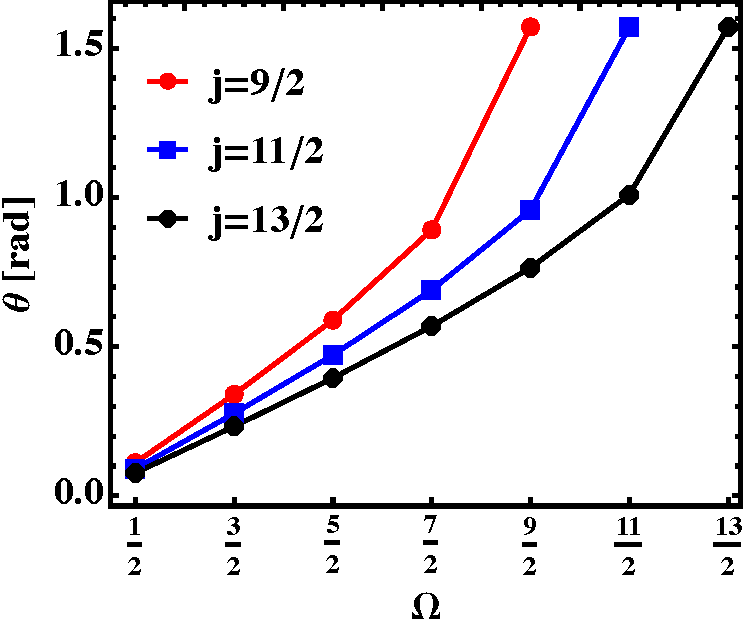
\includegraphics[scale=0.7]{Chapters/Figures/tilted_theta_shape.pdf}
    \caption{The change in $\theta$ with increasing values of $\Omega$, for given orbitals $j$.}
    \label{fig-tilting-angle-shape}
\end{figure}

The simplistic shapes within the splitting of an orbital $j$ into multiple sub-states (see Fig. \ref{nillson-orbits-splittings}) emerge from the considerations regarding the change in tilting angle $\theta$ and the observation that the difference in energy is rather slight (high) depending on low (high) $\Omega$ values.

Based on this discussion, it is clear that a full Nilsson diagrams is constructed with the configuration mixing of different $j$ values, configuration which is superimposed on state-splitting via the $\Omega$ projections. With this idea, one can state that \emph{no two lines in the Nilsson diagram with similar $\Omega$ values can cross each other}. As two such orbits come close to each other, they must repel as shown in Fig. \ref{fig-non-crossing}. Explaining the behavior of the lines that appear in the Nilsson diagrams \ref{nillson-diagram} - \ref{nillson-diagram-2} is straightforward: each line represents a Nilsson state, starting out in a straight line and then sloping downward or upward, depending on the angle of the orbit relative to the bulk nucleus. The \emph{curving} of an orbit starts when it approaches another level with the same quantum number $\Omega$ and parity $\pi$. Thus, the structure of any Nilsson diagram relies on three main features \cite{casten2000nuclear}:
\begin{itemize}
    \item the $\Omega$ splitting
    \item repulsion between two levels
    \item single-particle shell model energies
\end{itemize}

Taking a closer look at the second Nilsson diagram previously shown (see Fig. \ref{nillson-diagram-2}), there are two orbits within the 82-126 neutron shell that can be analyzed in terms of \emph{mixing}: $f_{7/2}$ and $h_{9/2}$. Obviously, the lack of deformation implies a degeneracy of these orbits, but when deformation occurs, splitting kicks in. The angle of the orbital orientation $\theta$ depends on the ratio $\frac{\Omega}{j}$ (recall formula $\theta=\arcsin\frac{\Omega}{j}\approx\frac{\Omega}{j}$ for low $\Omega$). 
Small tilting angles will occur due to i) small values of $\Omega$ or ii) high $j$. As a result, the energies for the orbits $\Omega=1/2,3/2,5/2$ belonging to the $h_{9/2}$ shell are decreasing in energy faster with deformation than those from $f_{7/2}$ orbit. Consequently, the different rates of decrease of the Nilsson energies will overcome any small spherical energy separation $f_{7/2}-h_{9/2}$, making the orbits with low $\Omega$ to approach each other: mixing becoming more pronounced.
But as discussed in the section devoted to \emph{two-state mixing}, two orbits defined by the same quantum numbers cannot cross each other, so the will repel, leading to the \emph{inflection point}. The points can be seen, for example, when looking at the $\Omega=5/2$ and $\Omega=7/2$ orbits, corresponding to $f_{7/2}$ and $h_{9/2}$, respectively.

Lastly, an alternative form of the Nilsson Hamiltonian should be expressed, taking into consideration the already studied nuclear radius (see Eq. \ref{nuclear-shape} which describes the shape of the nuclear surface) and the fact that until now, only the \emph{quadrupole} effects have been relevant to the discussion about deformed potentials in nuclei. Indeed, for quadrupole deformations, the nuclear radius can be simplified to:
\begin{align}
    R(\theta,\varphi)=R_0\left(1+\beta Y_2^0(\theta,\varphi)\right)\ .
    \label{simple-quadrupole-nuclear-surface}
\end{align}

The single-particle Hamiltonian can be written in the general form, starting from the expression Eq. \ref{eq-full-nilsson-ham}:
\begin{align}
    H_\text{Nil}=-\frac{\hbar^2}{2m}+\frac{1}{2}m(\omega_0r)^2-&\frac{4}{3}\sqrt{\frac{\pi}{5}}m(\omega_0r)^2\epsilon Y_2^0(\theta,\varphi)-2\kappa\hbar\omega_0(\vec{l}\cdot\vec{s})\nonumber\\
    &-2\kappa\hbar\omega_0\mu\left(l^2-\langle l^2\rangle_N\right)\ .
    \label{eq-nilsson-ham-spherical-harmonics}
\end{align}

The expression for the oscillator frequencies were already given (defined as functions of the deformation parameter $\epsilon$), and they keep the same form (see Eqs. \ref{oscillator-frequencies-nilsson} - \ref{omega-0-oscillator-frequency}). It is worth mentioning that both forms of $H_\text{Nil}$ are equivalent, and allow to describe the structure of the deformed nuclei in the limits of large deformations (via Eq. \ref{eq-full-nilsson-ham}) and small deformations (via Eq. \ref{eq-nilsson-ham-spherical-harmonics}). Within literature, the two parameters $\kappa$ and $\mu$ have usually values around $0.06$ for the former and $(0\sim 0.7)$ for the latter. As previously shown, the relationship between the $\epsilon$ and $\beta$ deformation parameters is given by $\epsilon=3/4\sqrt{5/\pi}\beta$.

When the deformations are small, $j$ is a good quantum number, and the Eq. \ref{eq-nilsson-ham-spherical-harmonics} represents a Hamiltonian for the AHO (which it was discussed) plus a \emph{perturbation} that is proportional to $\epsilon r^2Y_2^0$. One can consider the eigenstates of the Hamiltonian as some states labelled by the quantum numbers $Nlj$ and $m$ typical to the spherical case. Casten shows that if the angular part $Y_2^0$ is treated as a perturbation, it is possible to obtain a shift in energies relative to $\epsilon=0$ \cite{casten2000nuclear}:
\begin{align}
    \Delta E_{Nljm}=-\frac{4}{3}\sqrt{\frac{\pi}{5}}m\omega_2^0\epsilon\bra{Nljm}r^2Y_2^0\ket{Nljm}\ .
\end{align}

Furthermore, one can perform a separation of the radial and the angular parts while using the known relation for a harmonic oscillator potential:
\begin{align}
    \frac{1}{2}m\omega_0^2\bra{Nljm}r^2\ket{Nljm}=\frac{1}{2}\hbar\omega_0\left(N+\frac{3}{2}\right)\ ,
\end{align}
and, together with the evaluation of the matrix elements for spherical harmonics, the final expression for the energy shift at small deformations is:
\begin{align}
    \Delta E_{Nljm}=-\frac{2}{3}\hbar\omega_0\left(N+\frac{2}{3}\right)\epsilon\frac{\left[3K^2-j(j+1)\right]\left[\frac{3}{4}-j(j+1)\right]}{(2j-1)j(j+1)(2j+1)}\ ,
    \label{nilsson-energy-shifts}
\end{align}
with the projection of the total a.m. on the $z$ axis replacing the projection $m$. Based on Eq. \ref{nilsson-energy-shifts}, the following properties for a Nilsson diagram (within the small deformation regime) emerge:
\begin{itemize}
    \item There is a $K^2$ dependence for the energy shifts
    \item The quadrupole deformation parameter (albeit $\epsilon$ or $\beta$) shows a clear linear dependence for $\Delta E_{Nljm}$
    \item Another linear dependence for the shifts is induced by the principal (oscillator) quantum number $N$.
    \item When the deformation parameter is positive, there are more downward sloping orbits than upward ones. (Example discussed below)
\end{itemize}

For a value of $j$ greater than $1/2$, the terms $\left[3K^2-j(j+1)\right]$ and $3/4-j(j+1)$ are negative, resulting in the following types of orbits: \cite{krane1991introductory}:
\begin{align}
    \text{downward sloping:}&\ K<\sqrt{\frac{j(j+1)}{3}}=\frac{j}{1.8}\approx 0.65j\ ,\\
    \text{upward sloping:}&\ K>0.65j\ .
\end{align}

It was already shown that the angular orientation (i.e., the tilting angle $\theta$) of an orbit is given by $\theta=\arcsin(K/j)$. Checking to see for what value of $\theta$ the ratio $K/j=0.65$ corresponds to, this will lead to $\theta=40^\circ$. Consequently, the physical implication is that any larger \emph{tilt} of an orbit within a prolate quadrupole deformation is energetically unfavorable. In Fig. \ref{fig-nilsson-delta-E-shift} two different $j$ orbits, namely $h_{9/2}$ and $i_{13/2}$ are studied in terms of their energy shifts according to Eq. \ref{nilsson-energy-shifts}. It can be seen that indeed, there are more downward sloping orbitals, since the quadrupole deformation parameter has been set to a positive value $\epsilon=0.22$.

\begin{figure}
    \centering
    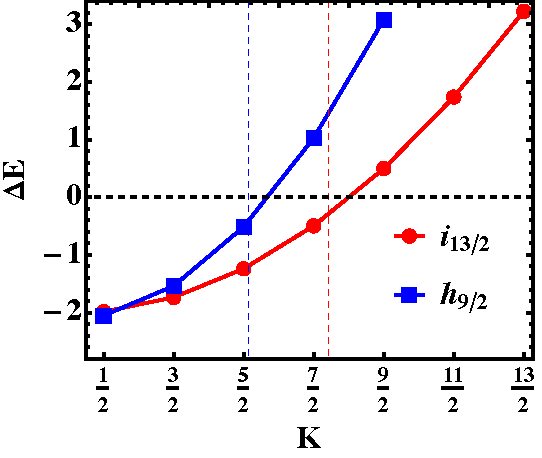
\includegraphics[scale=0.65]{Chapters/Figures/energy_shift_nilssonDeltaE.pdf}
    \caption{The energy shift $\Delta E$ for two orbits: $h_{9/2}$ and $i_{13/2}$ for a given deformation $\epsilon=0.22$. The dashed vertical lines (colored) represent the value for $K$ where the `change' from downward sloping curves to upward sloping curves takes place (that is $K\approx 0.65j$). This is just an illustrative example inspired from the discussion regarding single-particle orbits in Ref. \cite{casten2000nuclear}}
    \label{fig-nilsson-delta-E-shift}
\end{figure}

There is another important physical consequence emerging from the four main characteristics mentioned above, based on the principal quantum number $N$. The dependence on $N$ will imply that the slopes of any Nilsson energy level will be \emph{steeper} as $N$ has large values. As such, heavier nuclei will tend to deform much easier than lighter ones. The explanation for the influence of large $N$ on the steepness was done in Refs. \cite{bohr1998nuclear,krane1991introductory,casten2000nuclear}. Shortly, a nucleon belonging to a high oscillator shell will have a large average radius (the expectation value of $r^2$ was done in Eq. \ref{nilsson-energy-shifts} via the expression $\langle r^2 \rangle=(N+3/2)$ \cite{bertulani2007nuclear}). As the nucleus deforms, the density distribution of the nuclear matter will approach that orbit. The effect on the orbiting nucleon to decrease its energy rapidly as the nuclear matter comes closer to the orbit is due to the \emph{attractive} nature of the nuclear force itself. 
Clearly, this effect is less obvious for a particle in a lower oscillator shell that is already very close to the rest of the nuclear matter.

The centrifugal $\vec{l}^2$ and spin-orbit $\vec{l}\cdot\vec{s}$ terms from Eq. \ref{eq-nilsson-ham-spherical-harmonics} will become negligible in the limit of \emph{large deformation}, such that the Nilsson Hamiltonian will reduce to the known AHO-like form. In this special case, the motion will separate into \emph{independent} oscillations in the direction of the symmetry axis and the perpendicular plane (i.e., in the direction of $z$-axis and $xy$ plane). Consequently, the good quantum numbers for this kind of situation are the $n_z$ and $(n_x+n_y)$ oscillator quantum numbers. Since the eigenvalues for a one-dimensional (and, implicitly for the three-dimensional) harmonic oscillator are established, the energy spectrum for single-particle orbits in the regime of large $\epsilon$ (or, equivalently $\beta$) will be given by:
\begin{align}
    E_{n_x,n_y,n_z}=\hbar\omega_x(N-n_z+1)+\hbar\omega_z\left(n_z+\frac{1}{2}\right)\ .
\end{align}

The remarking feature of the Hamiltonian which corresponds to this set of eigenvalues is its invariance to rotations about the $z$ axis. The projections for the particle's orbital and spin a.m. are constants of motion. As it was previously discussed, the sum of the two projections $\Lambda$ and $\Sigma$ is indeed $\Omega$ or equivalently $K$ in the case of $\vec{R}$ being perpendicular to the $z$-axis.

With this, the description of the Nilsson Deformed Model is clear enough for understanding it and also be able to justify its importance within the rest of the present work. It will be shown that based on the so-called Particle-Rotor-Model \cite{bohr1998nuclear,davydov1958rotational}, it plays a crucial role in determining the Hamiltonians that are specific to the phenomena (and implicitly the nuclei) of interest.

\section{Collective Model}

Although the previous single-particle model is able to successfully treat many nuclei (e.g., those which are lie near closed shells), the single-nucleon motion within a (deformed) potential is not enough to describe for example: nuclear fission, values for quadrupole moments of multiple deformed nuclei \cite{townes1949nuclear} or lifetime measurements that through single-particle calculations fail to reproduce experimental data on some gamma-ray transitions (of electric quadrupole type) \cite{goldhaber1951classification}.

The collective model is one of the most `complete' tools in describing the nuclear phenomena across the chart of nuclides. It brought tremendous progress within nuclear community in order to validate but also predict nuclear behavior in the high-spin limit for example. A major feature of this model is the introduction of the so-called \emph{rotational bands}, characteristic of deformed nuclei which will be discussed in detail later on, since it is of crucial interest to this work.

Developed by Bohr and Mottelson \cite{bohr1953collective,bohr1998nuclear} more than 50 years ago the Nuclear Collective Model, it is based on the Liquid-Drop-Model (which formulated by Niels Bohr \cite{bohr1936neutron}). Moreover, the predictions for nuclear deformation made by Rainwater \cite{rainwater1950nuclear} played another fundamental role in the model's development. The basic assumption within this model is that the nuclear density distribution can be approximated as a droplet of nuclear matter which has shape-specific degrees of freedom. This nuclear droplet is also capable of vibrating and rotating (remember the discussion from Chapter \ref{chapter-2}, where the nuclear radius was described in terms of some \emph{collective coordinates}: the coordinates dictate the shape evolution with time, letting the entire shape to vibrate and rotate.)

\subsection{Bohr Hamiltonian}

As a first step, the concept of a nuclear liquid drop is used to construct the Hamiltonian of the problem. The droplet is said to exhibit excitations shape (or surface) oscillations which have a dynamical character. These shape oscillations are illustrated in Fig. \ref{fig-nuclear-vibration}, where one can interpret that as a vibrating nucleus with a spherical equilibrium shape. Since the collective coordinates are time-dependent, at each moment in time, the nuclear radius $R$ at moment $t$ will locate a point on the surface in the direction given by the radial coordinates $\theta,\varphi$.
\begin{figure}
    \centering
    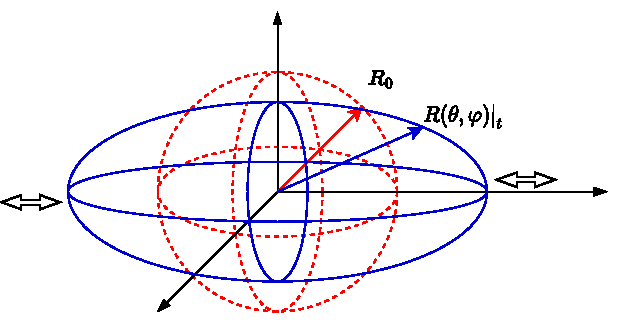
\includegraphics[scale=1.1]{Chapters/Figures/shape_oscillations.pdf}
    \caption{The vibration of a nucleus whose equilibrium shape is a spheroid, with nuclear radius $R_0$ (\emph{average nuclear radius}) and the nuclear radius at a different moment in time.}
    \label{fig-nuclear-vibration}
\end{figure}

By using Eq. \ref{nuclear-shape} which characterizes the \emph{vibrations} of a nuclear surface (via the collective coordinates $\alpha_{\lambda\mu}$), one can give the expression of an initial Hamiltonian of \emph{collective} nature as:
\begin{align}
    H_\text{coll}\equiv T+V=\frac{1}{2}\sum_{\lambda\mu}\left[B_\lambda\left|\frac{\text{d}\alpha_{\lambda\mu}}{\text{d}t}\right|^2+C_\lambda|\alpha_{\lambda\mu}|^2\right]\ ,
    \label{collective-hamiltonian-stiffness-inertia}
\end{align}
Hamiltonian which is in fact both invariant under rotation and time reversal \cite{messiah2014quantum}.  The real numbers $B_\lambda$ and $C_\lambda$ represent \emph{inertial} and \emph{stiffness} parameters for the nuclear matter. The spectrum of such a Hamiltonian after a canonical quantization (see calculations in Ref. \cite{ring2004nuclear} or \cite{bertulani2007nuclear}) will have a harmonic-like structure, depending on the value of $\lambda$. Indeed, by looking at the expression from Eq. \ref{collective-hamiltonian-stiffness-inertia} one can see that it can be brought to a form:
\begin{align}
    H_\text{coll}^\text{osc}=\frac{p^2}{2m}+\frac{1}{2}kr^2\ ,
    \label{eq-bohr-hamiltonian-oscillator-simple}
\end{align}
which is typical to a harmonic oscillator Hamiltonian. The frequency of oscillation of such a Hamiltonian is given by the relation $\omega=\sqrt{k/m}$. The vibrations can now be understood in terms of a sum of harmonic oscillator frequencies, where each frequency is given by $\lambda$:
\begin{align}
\omega_\lambda=\sqrt{\frac{C_\lambda}{B_\lambda}}\ .
\end{align}

The inertia term $B_\lambda$ (also called the \emph{mass parameter}) has the following expression \cite{ring2004nuclear}:
\begin{align}
    B_\lambda=\frac{\rho mR_0^5}{\lambda}=\frac{3}{4\pi\lambda}AmR_0^2\ ,
\end{align}
showing a quadratic dependence with the average nuclear radius. With these ingredients, one can sketch a form of $H_\text{coll}$ similar to Eq. \ref{eq-bohr-hamiltonian-oscillator-simple} in the following manner:
\begin{align}
    H_\text{coll}=\sum_{\lambda\mu}\hbar\omega_\lambda\left(N_{\lambda\mu}+\frac{1}{2}\right)\ ,
\end{align}
where indeed, the typical harmonic oscillator spectrum should be expected for the final collective spectra of nuclei.

The recipe for further manipulation of the Bohr's collective Hamiltonian from Eq. \ref{collective-hamiltonian-stiffness-inertia} is quite a lengthy process \cite{bohr1998nuclear,ring2004nuclear}, with several considerations that are beyond the scope of the current work. Shortly, for the quadrupole deformed nuclei, the expression of the potential term $V$ will be a function that depends on the parameters $(\beta,\gamma)$, potential that is defined as a quadratic approximation in the vicinity of a deformed minimum point $p_0|_\text{min}=(\beta_,\gamma_0)$. This starts from the general assumption that the nucleus has the deformation $p_0$ in the ground state, and the excitations are rotations and small oscillations around this \emph{equilibrium} deformation point. Thus $V(\beta,\gamma)$ can be written as:
\begin{align}
    V(\beta,\gamma)=\frac{1}{2}C_{20}\left(\alpha_{20}(\beta,\gamma)-\alpha_{20}^2\right)^2+\frac{1}{2}C_{22}\left(\alpha_{22}(\beta,\gamma)-\alpha_{22}^0\right)\ .
    \label{bohr-collective-potential}
\end{align}

Choosing the body-fixed axis as a reference system makes the calculations much easier, since the system's axes coincide with the principal axes of the ellipsoid itself. Assuming such a coordinate system and an ellipsoid which possesses axial symmetry, one can write the kinetic term $T$ of the Hamiltonian as a sum of a \emph{rotational} and a \emph{vibrational} part.
\begin{align}
    T=T_\text{vib}+T_\text{rot}\ .
\end{align}

The equations for the two sub-terms are thoroughly demonstrated in Ref. \cite{li2022model}. Their expressions are given in terms of the deformation parameters $(\beta,\gamma)$, the mass parameters $B_2$ (for the quadrupole deformations) and the stiffness parameters $C_2$. Thus, the vibrational term is:
\begin{align}
    T_\text{vib}=\frac{1}{2}B_2\left(\dot{\beta}^2+\beta^2\dot{\gamma}^2\right)\ ,
    \label{kinetic-vibrational-energy-collective}
\end{align}
and the rotational term is:
\begin{align}
    T_\text{rot}=\frac{1}{2}\sum_i\mathcal{I}_i\omega_i^2\ ,
    \label{kinetic-rotational-energy-collective}
\end{align}
where the index $i=1,2,3$ suggests each of the three principal axes of the ellipsoid (this notation is different from the previous notations $x,y,z$ and it will always suggest the body-fixed system). In the expression of $T_\text{rot}$, two crucial physical quantities arise, namely the angular velocities around each body-fixed axis and the functions $\mathcal{I}_k$ that will eventually play the role of \emph{moments of inertia}. However, it is important to analyze the functions $\mathcal{I}_k(\beta,\gamma$) in order to better understand what kind of nature the nucleus exhibit in its rotational and vibrational motion. Ref. \cite{ring2004nuclear} shows that:
\begin{align}
    \mathcal{I}_k=4B_2\beta^2\sin^2\left(\gamma-\frac{2\pi}{3}k\right)\ .
\end{align}

In the case of fixed deformation (that is $\beta$ and $\gamma$ do not change), then the rotational kinetic term represents the energy of a rotor with the moments of inertia $\mathcal{I}_{1,2,3}$, i.e., a \emph{pure rotor}. When the deformation parameters are changing, the rotational and vibrational degrees of freedom will become coupled by the deformation dependence of $\mathcal{I}_k$, leading to a situation that is not specific to a pure rotor. In fact, the functions $\mathcal{I}_k$ will not represent the moments of inertia (MOI) for a rigid rotor anymore. However, a comparison between $\mathcal{I}$, the rigid-like $\mathcal{I}_k^\text{rig}$ MOI, and irrotational-like MOI $\mathcal{I}_k^\text{irr}$ is done experimentally, from determinations of the energy spacing between the first excited states. The last two quantities have the following expressions \cite{bohr1954rotational,ring2004nuclear}:
\begin{align}
    \mathcal{I}_k^\text{rig}&=\frac{2}{5}mAR_0^2\left(1-\sqrt{\frac{5}{4\pi}\beta\cos\left(\gamma-\frac{2\pi}{3}k\right)}\right)\ ,\\
    \mathcal{I}_k^\text{irr}&=\frac{3}{2\pi}mAR_0^2\beta^2\sin^2\left(\gamma-\frac{2\pi}{3}k\right)\ .
    \label{eq-irrotational-rigid-mois}
\end{align}

The dependence of the two types of MOI on the triaxiality parameter $\gamma$ (and fixed $\beta$) can be seen in Fig. \ref{fig-irrotational-rigid-mois}. The differences between the irrotational-like and rigid MOI are as follow:
\begin{itemize}
    \item The irrotational MOI vanish when the ellipsoid has axial symmetry
    \item $\mathcal{I}^\text{irr}$ is much more sensitive to the deformation $\beta$, while the rigid MOI have most of the contribution coming from a typical rigid sphere-like MOI
    \item Determinations of the \emph{experimental} MOI for well-deformed nuclei show that the irrotational MOI is smaller by a factor of almost 3 than the experimental values. Moreover, the rigid MOI show a factor of 2 larger than the experimental values:
    \begin{align}
        \mathcal{I}^\text{irr}<\mathcal{I}^\text{exp}<\mathcal{I}^\text{rig}\ ,
    \end{align}
    suggesting that the \emph{real} flow structure within a nucleus is neither irrotational, nor like a rigid rotator.
\end{itemize}

\begin{figure}
    \centering
    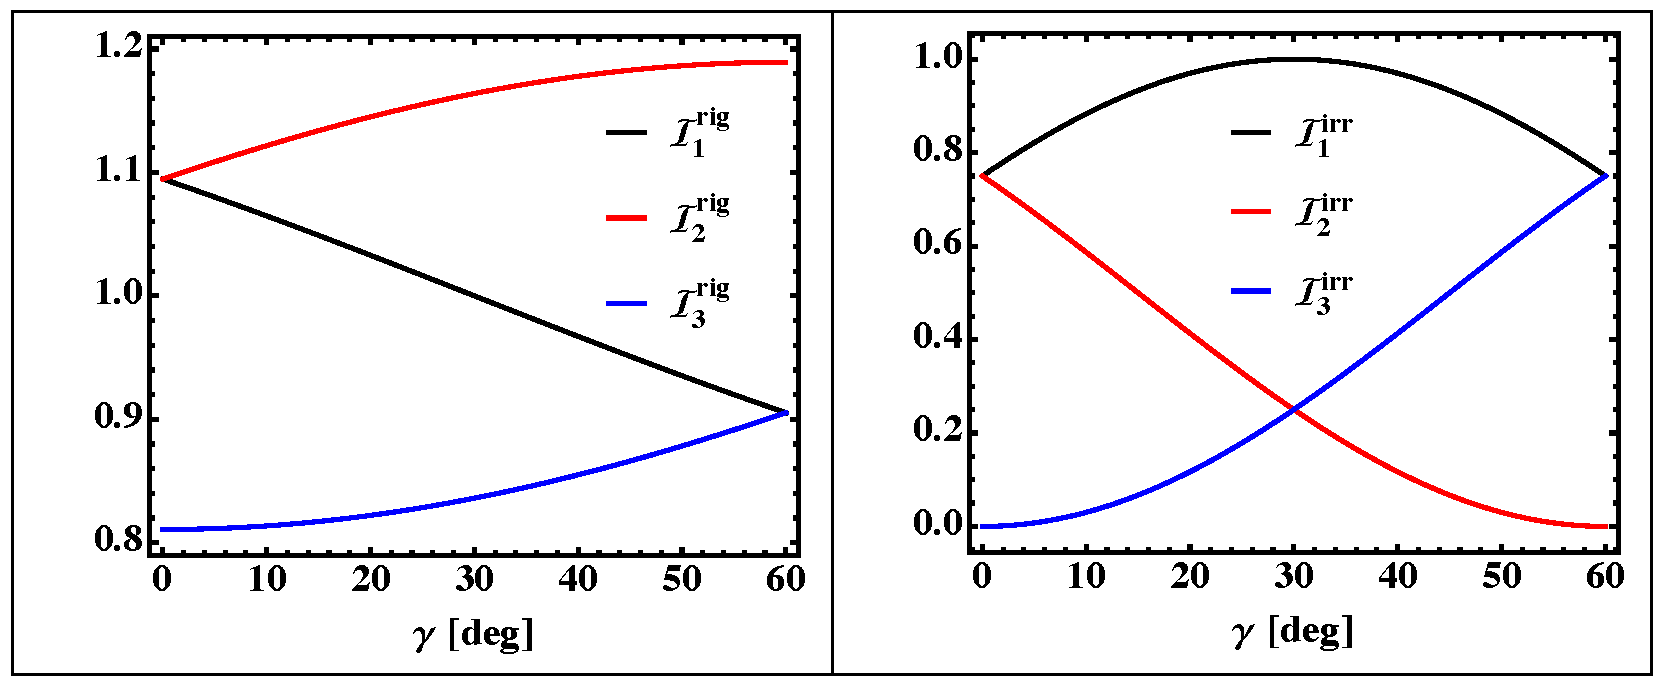
\includegraphics[scale=0.51]{Chapters/Figures/mois_rig_irr.pdf}
    \caption{Comparison between the irrotational-like and the rigid-like MOI defined in Eq. \ref{eq-irrotational-rigid-mois} that are typical for a rigid rotator or the irrotational motion of a fluid. The deformation parameter $\beta$ is $0.3$. Note the vanishing of the irrotational MOI when axial symmetry is present.}
    \label{fig-irrotational-rigid-mois}
\end{figure}

\subsection{Nuclear Vibration}

The energy scheme is composed of levels that are built from these oscillator frequencies. The absorption or emission of vibration-like energy quanta (i.e., phonons) that a nucleus can do (passing to a higher or a lower level) will be in terms of dipole, quadrupole, octupole, etc. vibrating phonons. These excitations will contribute to building the entire spectrum of the nuclei, starting with the ground state: resulting in the so-called \emph{vibrational bands}.
Since the the quadrupole effects are of interest within the current work, the vibrational spectrum specific to quadrupole $\lambda=2$ phonons can be seen in Fig. \ref{fig-vibrational-bands}.
\begin{figure}
    \centering
    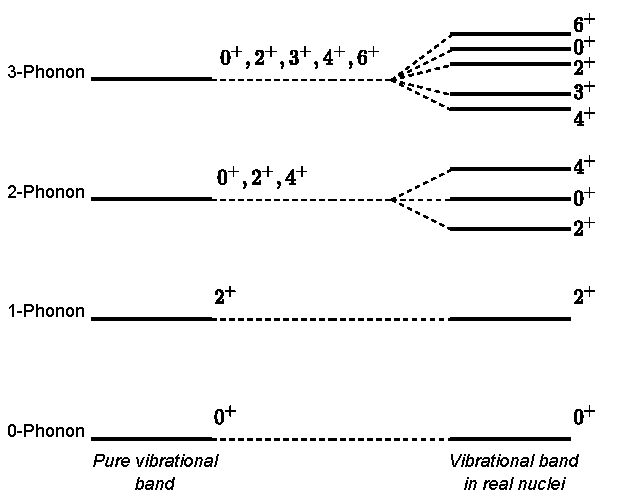
\includegraphics[scale=1.1]{Chapters/Figures/vibrational_states.pdf}
    \caption{An illustrative example with vibrational bands that are built as excitations of multiple phonons on a ground state. The left side contains an ideal harmonic vibrator, with the degenerate spin states indicated for each level. Right side contains the non-degenerate vibrational levels that exist in nuclei. Keep in mind that the each phonon level is built as multiple excitations of a \emph{quadrupole phonon}.}
    \label{fig-vibrational-bands}
\end{figure}

A general rule that is used to construct such vibrational bands is related to the concept of \emph{symmetrized states}. Since the excited quanta are represented by phonons (identical bosons) which have integer angular momentum (e.g., $\lambda=2$ for the quadrupole vibrations) the only spin states than can be observed in such spectra are the ones for which the final angular momenta couple to give symmetric combinations. This is the reason why in the energy state created by exciting the ground state $0^+$ with two phonons, only the states $0^+,2^+,4^+$ appear; the spin states $1^+$ and $3^+$ do not give symmetric combinations. A more generic method for determining which sequence of spins can be obtained by coupling angular momenta of vibrational phonons can be seen in Ref. \cite{ring2004nuclear}.

A quantity which is often used within the measurements of nuclear properties is the ratio between the second and the first excited states within a band. These ratios are usually denoted by $E(4^+)/E(2^+)$ (the state $4^+$ belongs to the triplet phonon state depicted in Fig. \ref{fig-vibrational-bands}), and the theoretical value for the vibrational model gives a value of $2$. However, some experimental results point out to a value close to $2.2$ for nuclei below $A=150$, and a constant value of $3.3$ for $150<A<190$ (refer to Fig. \ref{4state-2state-ratio}). It should be noted that for the latter case, the value of the ratio is specific to another kind of nucleonic motion: \emph{rotation}, which will be discussed in the following section.
Example of experimental \emph{vibrational bands} for several even-$A$ nuclei are shown in Fig. \ref{energy-levels-120Te-virbational-band}.

\begin{figure}
    \centering
    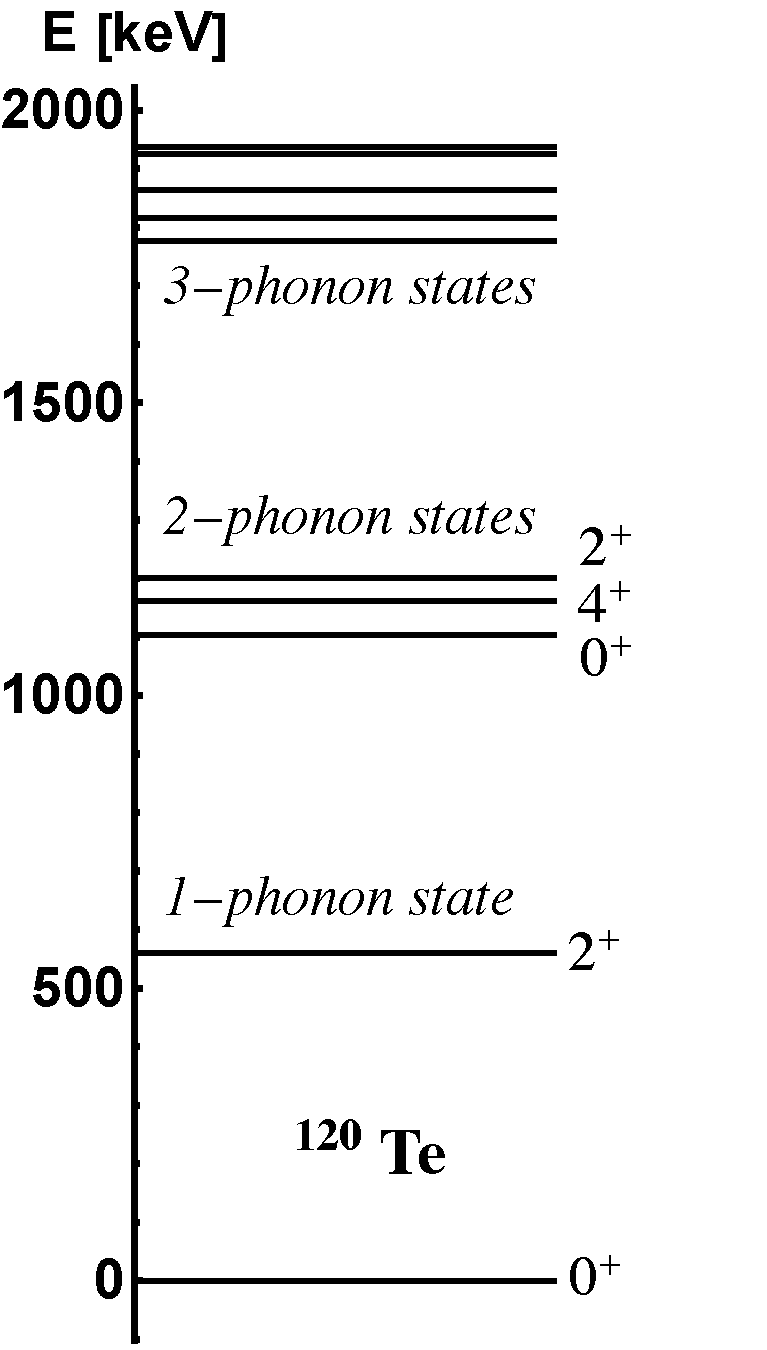
\includegraphics[scale=0.37]{Chapters/Figures/120Te_vib_experimental.pdf}
    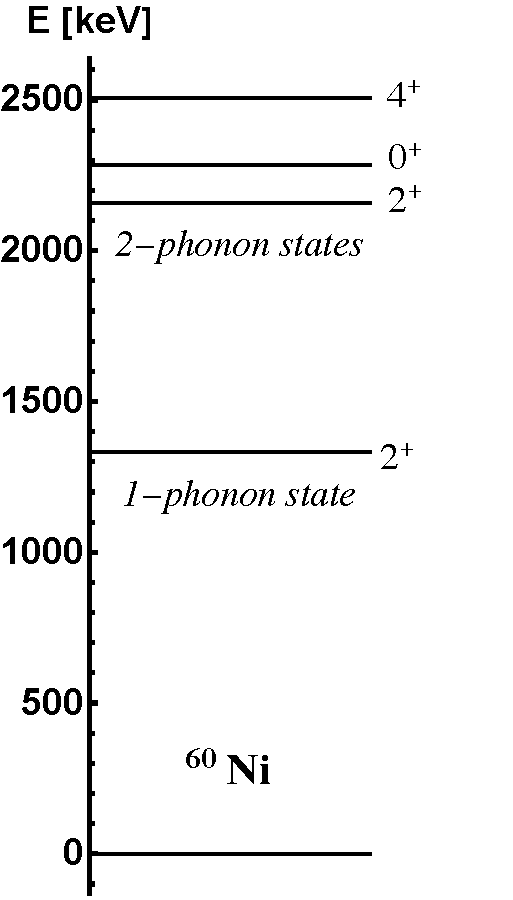
\includegraphics[scale=0.55]{Chapters/Figures/60Ni_vib_experimental.pdf}
    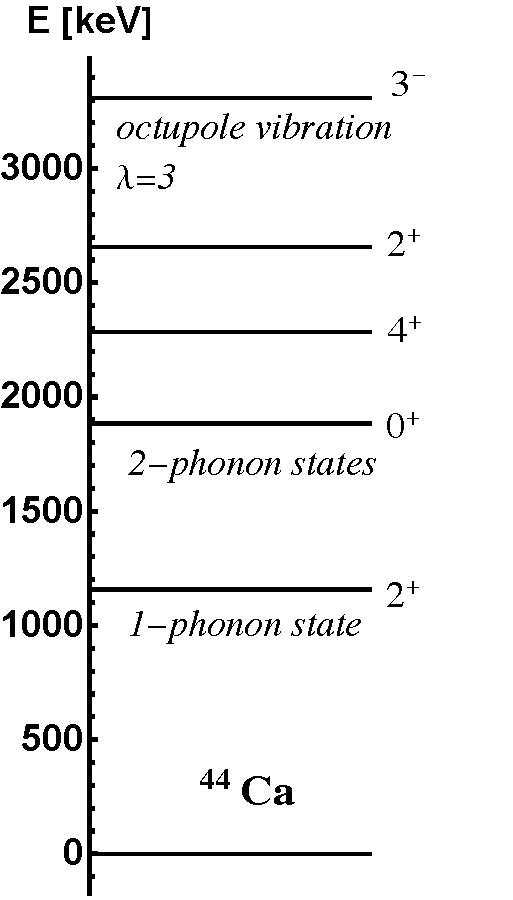
\includegraphics[scale=0.55]{Chapters/Figures/44Ca_vib_experimental.pdf}
    \caption{Vibrational bands in even-$A$ nuclei. \textbf{Left:} The experimental energy levels for $^{120}$Te, showing a vibrational structure for this nucleus. The triplet states that correspond to two excited quadrupole phonons can be seen, together with the quintuplet formed by adding three phonons to the $0^+$ ground state. Experimental data is taken from \cite{kitao2002nuclear}. \textbf{Middle:} The experimental data for $^{60}$Ni. For simplicity, only the first two phonon states are represented. Experimental data for this nucleus was taken from Ref. \cite{browne2013nuclear}. \textbf{Right}: The experimental data for a vibrational-like structure in $^{44}$Ca. Data is taken from Ref \cite{chen2011nuclear}. For the last spectrum, one can observe an energy level coming from the vibrational motion corresponding to an \emph{octupole} mode ($\lambda=3$).}
    % \label{energy-levels-60Ni-virbational-band}    
    \label{energy-levels-120Te-virbational-band}    
\end{figure}

There can also be vibrational bands in odd-$A$ nuclei. Indeed, if one considers the nucleus as a spherical even-even core plus an extra nucleon, the \emph{final} nuclear states are formed by coupling an individual $j$ orbit with the vibrational states of the core.
In the case of odd-$A$ nuclei, one can take the case of $^{63}$Cu, which has the ground state $3/2^{-}$. The g.s. for this nucleus is given by the last \emph{uncoupled} nucleon that occupies a shell. In fact, for this particular nucleus, it is the $2p_{3/2}$ proton that will give the final spin and parity of the nucleus. The vibrational spectrum which arises here can be explained by coupling the aforementioned proton with the even-$A$ core of $^{62}$Ni. Indeed, by taking a $2^+$ vibrational phonon from the even nucleus, then the (odd-proton)+(phonon) system can generate a sequence of energy states that are given by the angular momenta coupling rules (i.e., negative parity states with $I=1/2,3/2,5/2,7/2$ will be formed).
This kind of particle-core coupling that generates sequences of bands will be relevant later on, when discussing the formalism of this work.
The energy levels depicted in Fig. \ref{energy-levels-63Cu-virbational-band} show the particle-core coupling effects on the vibrational structure in odd-mass nuclei.

\begin{figure}
    \centering
    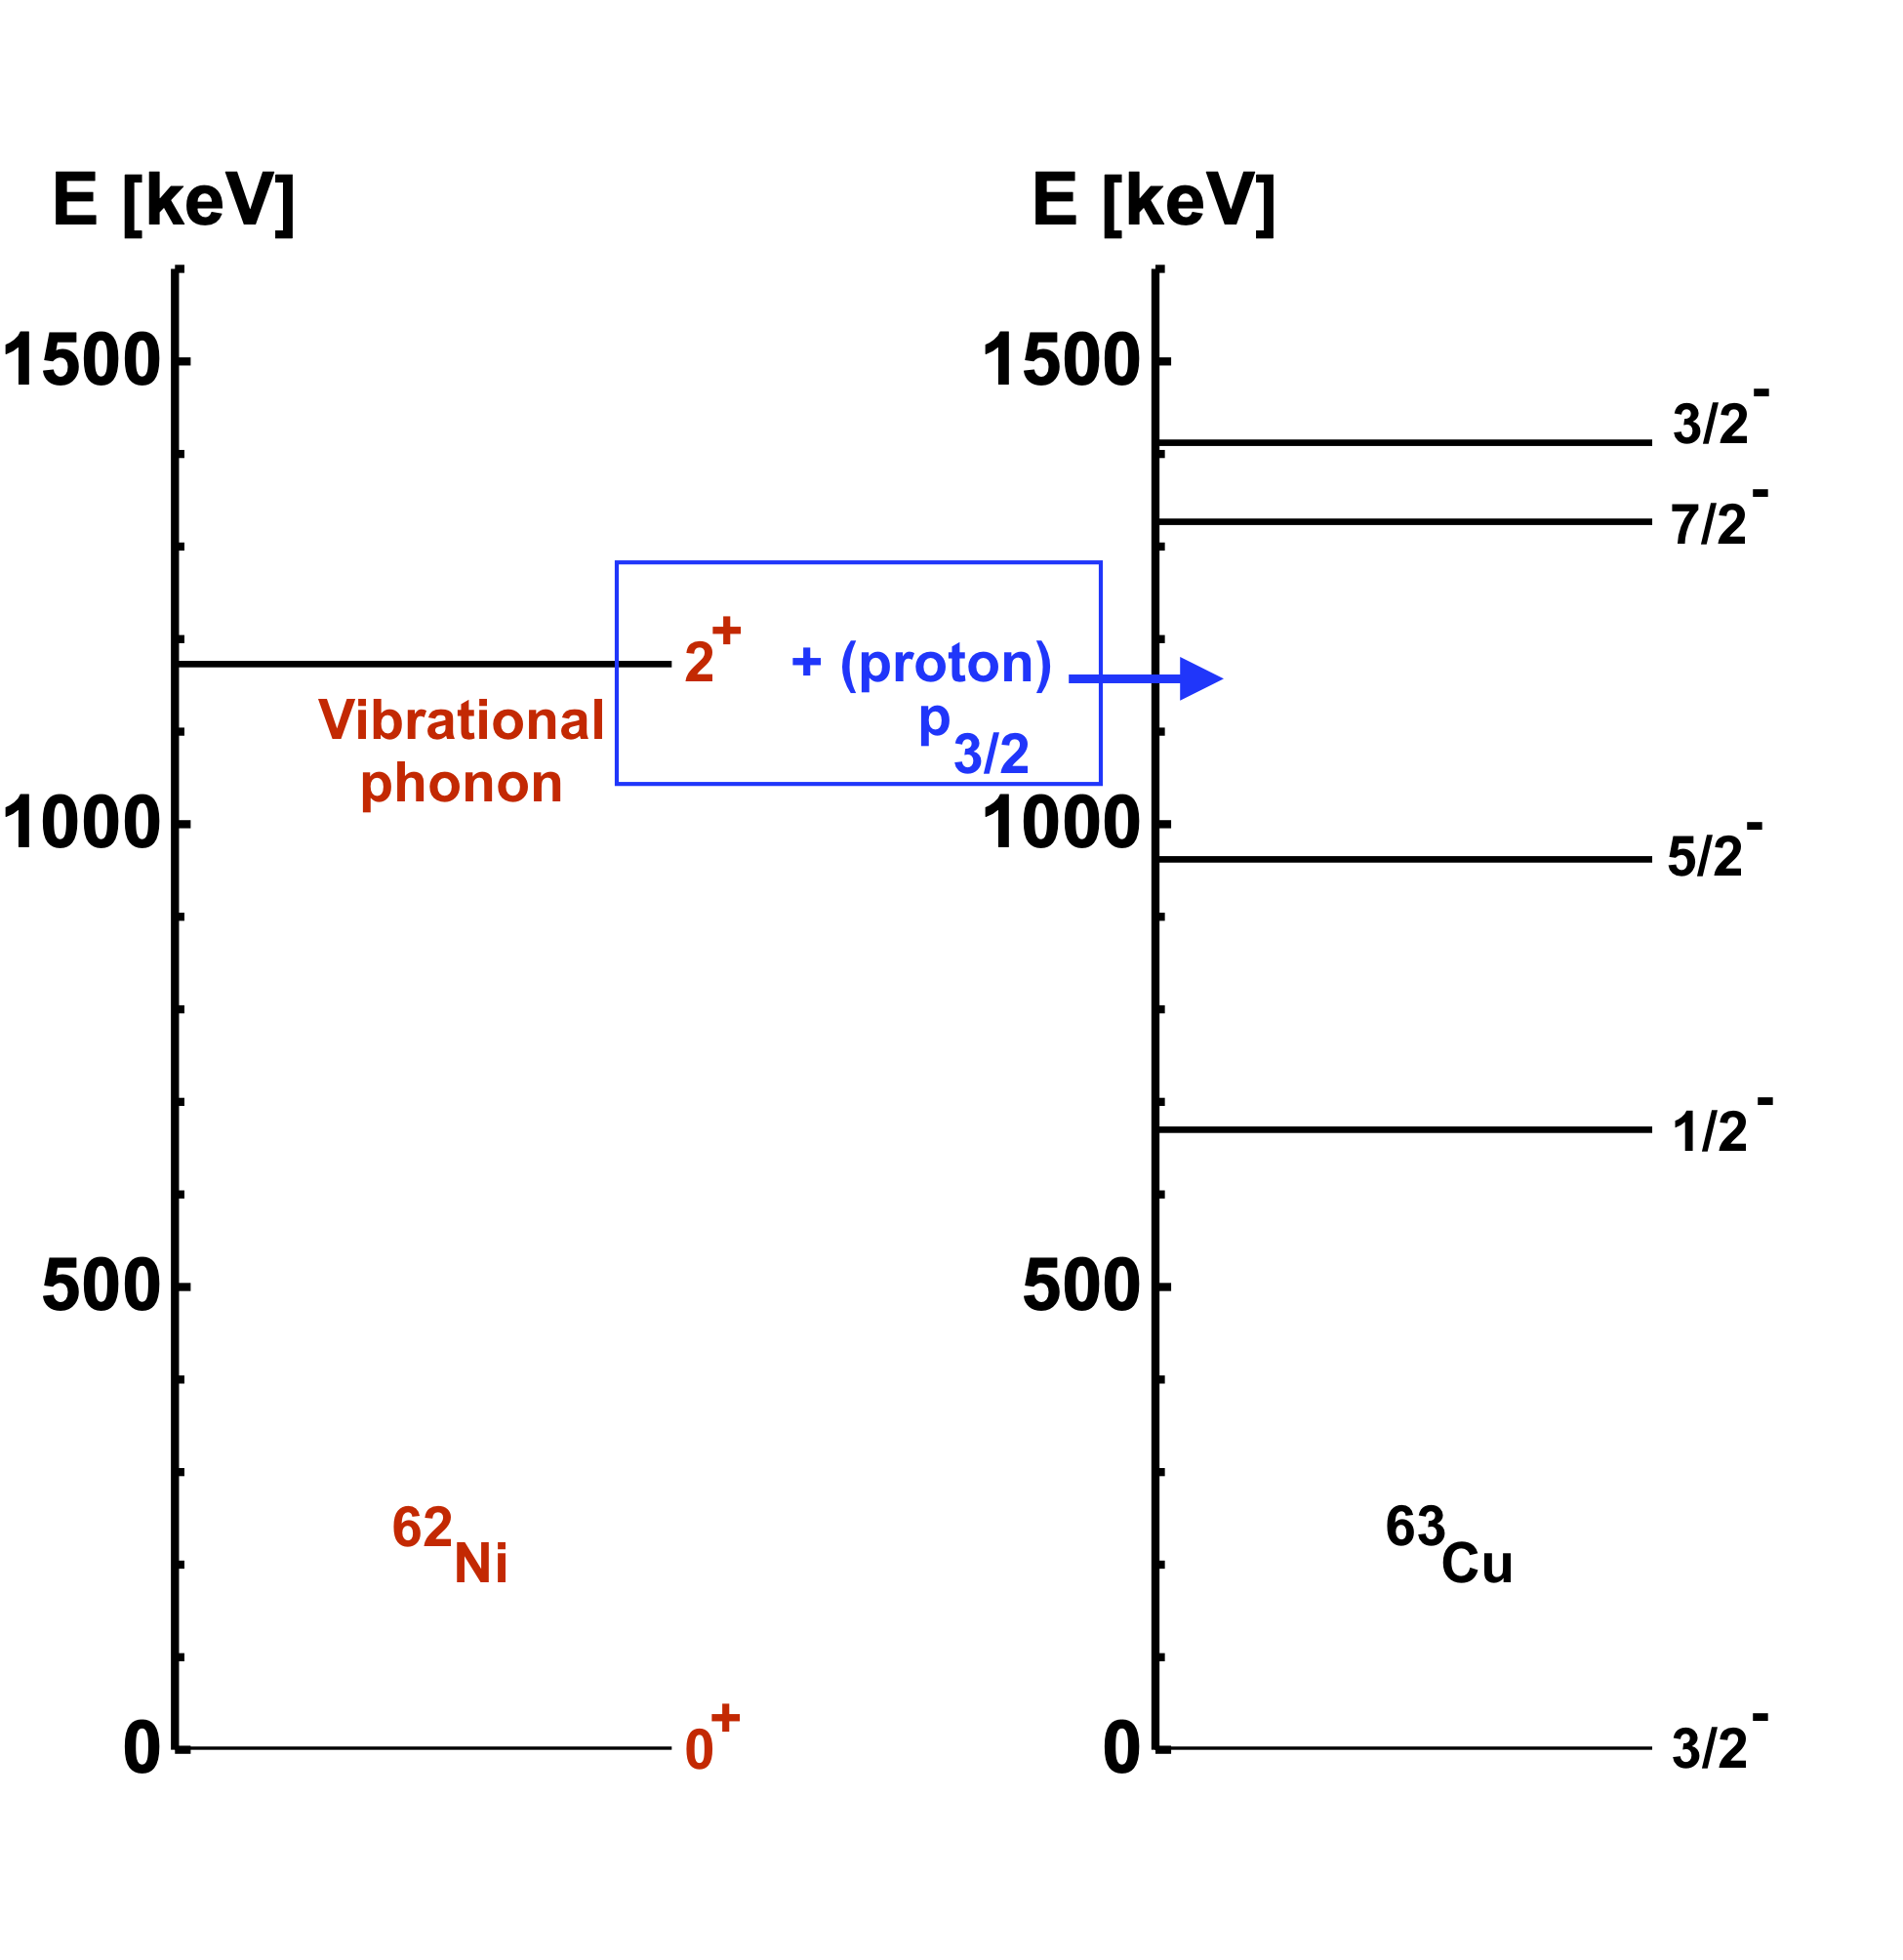
\includegraphics[scale=0.155]{Chapters/Figures/63Cu_vib_experimental.png}
    \caption{The experimental data of the vibrational states in $^{63}$Cu. The $2^+$ phonon state in $^{62}$Ni is also shown for a clearer picture. The experimental data for $^{62}$Ni was taken from Ref. \cite{nichols2012nuclear} and for $^{63}$Cu was taken from Ref. \cite{erjun2001nuclear}. The blue rectangle tries to emphasize that the states quadruplet is formed by the coupling of odd proton to the $2^+$ vibrational state from the neighboring nucleus.}
    \label{energy-levels-63Cu-virbational-band}
\end{figure}

Since the quadrupole vibrations carry an angular momentum of 2 units, there can be two types of vibrations in a deformed nucleus: one which corresponds to $K=0$ and one for $K=2$. For $K=0$ the vibrational motion is called $\beta$-vibration, and this induces an small fluctuations in the quadrupole deformation parameter, but it preserves the axial symmetry of the nucleus (the vibration is aligned with the deformed axis).

The second type of vibration (for $K=2$) is called the $\gamma$-vibration which is responsible for fluctuations in the triaxiality parameter $\gamma$. A qualitative description for such an oscillation can be explained in terms of a physical object such as an american football \cite{krane1991introductory}: if one pictures a nucleus with such a shape, then $\gamma$-vibrations will result in the simultaneous pushing and pulling of the ball on its sides, while the former vibrational mode will correspond to continuous pushing and pulling on the ends of the football. An illustration which aims at explaining the geometrical meaning of the $\beta$ and $\gamma$ vibrations in nuclei can be seen in Fig. \ref{rotation-vibration-geometrics}.

\begin{figure}
    \centering
    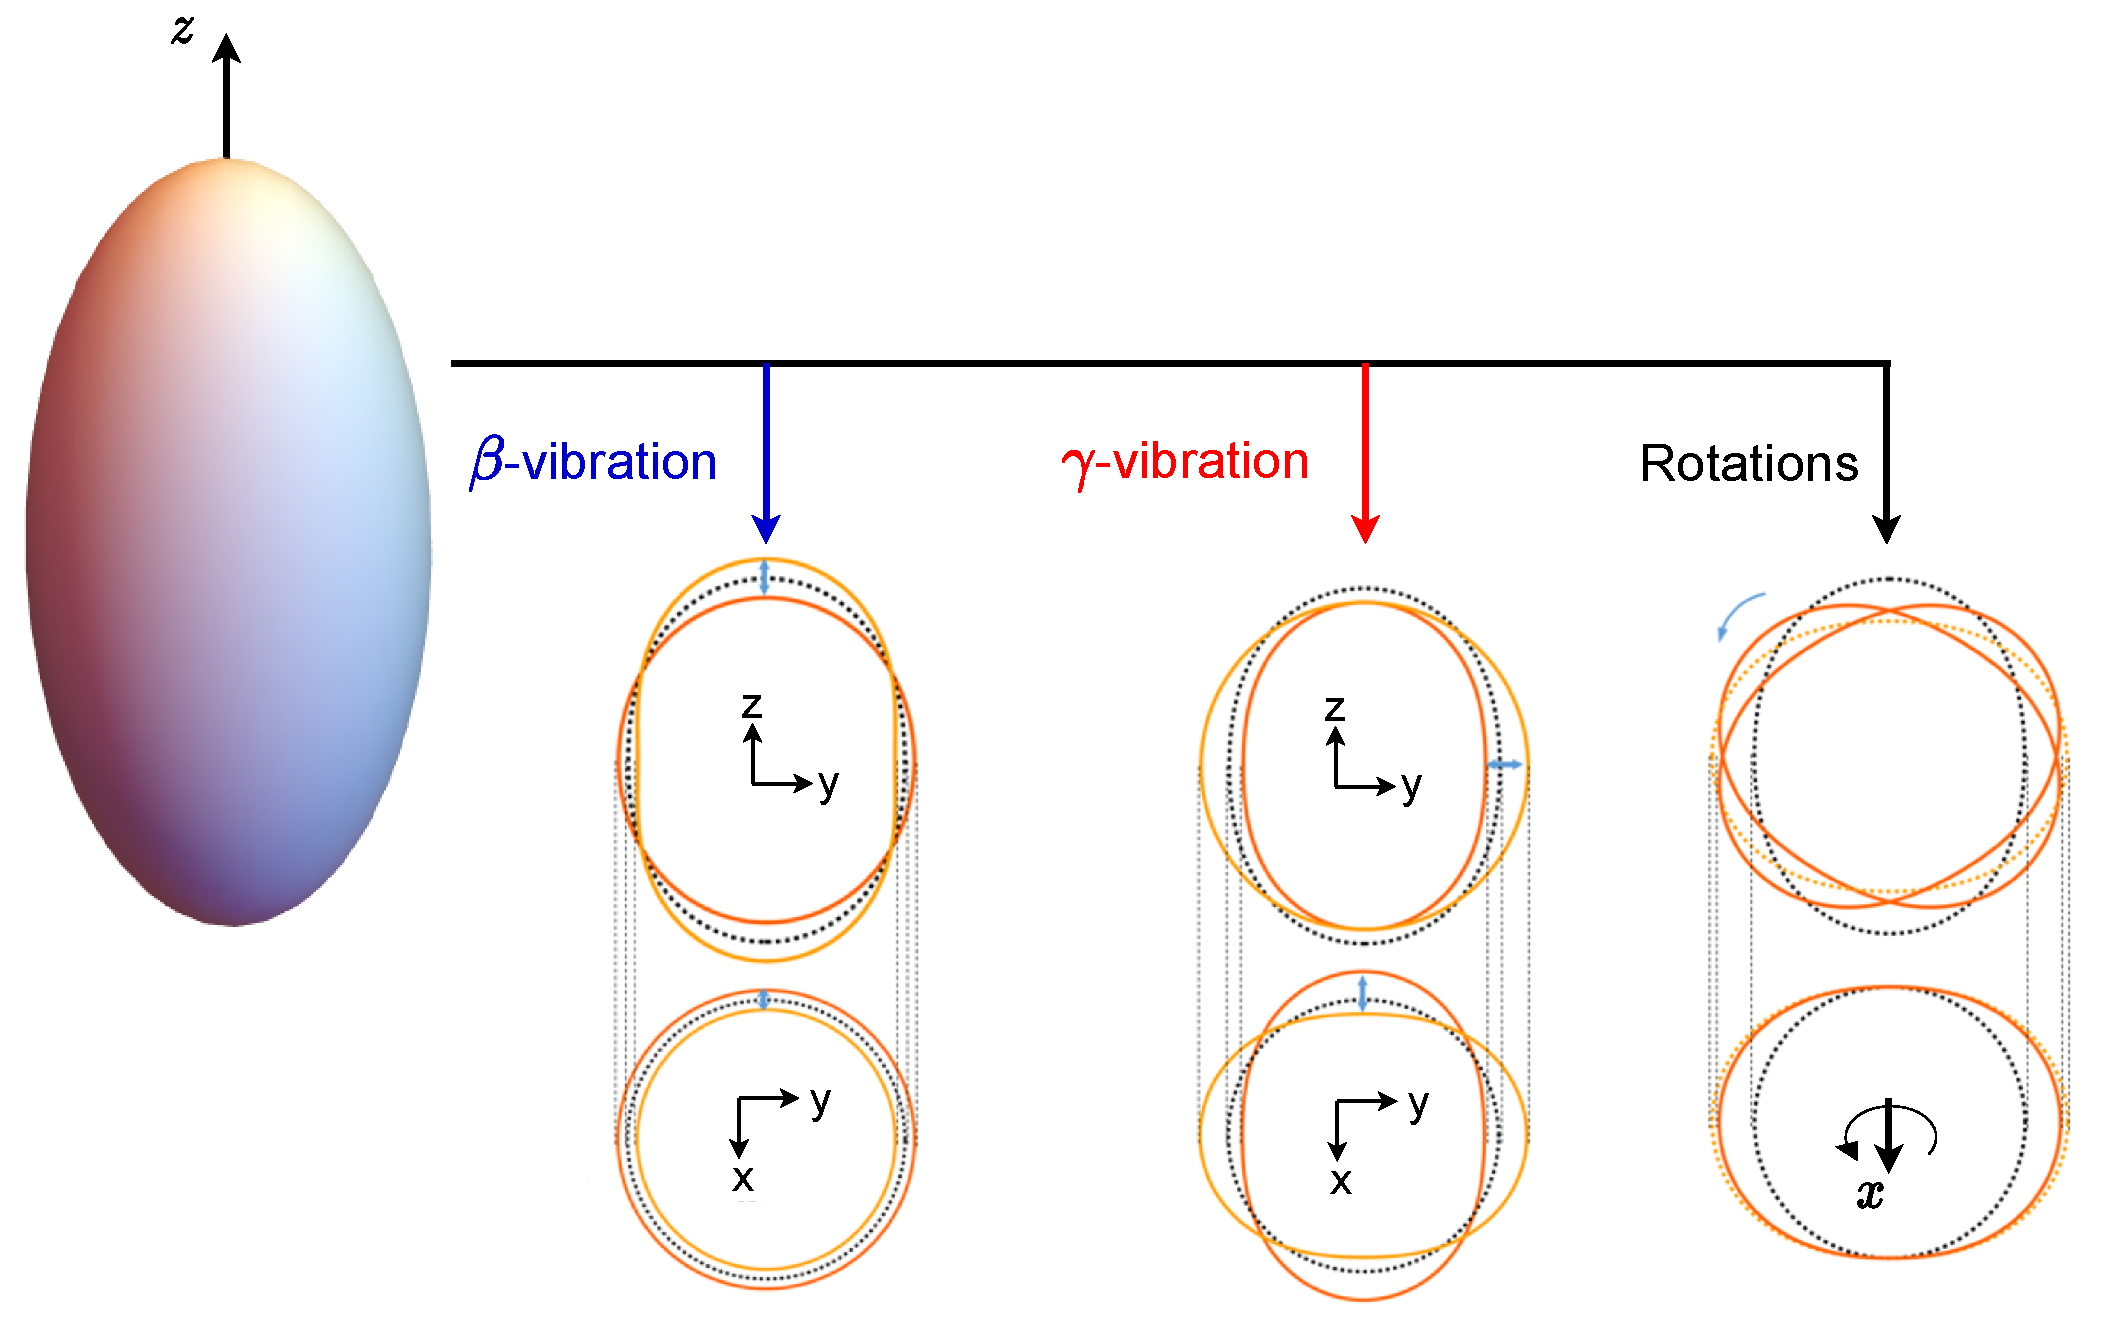
\includegraphics[scale=0.405]{Chapters/Figures/rotationsVibrations_Rotations.pdf}
    \caption{A sketch which shows the two types of vibrations in nuclei. The initial nucleus in this example is of prolate type. Each mode of vibration is visualized from the side-view and top-view, respectively. This figure was inspired (and also contains graphical elements) from Ref. \cite{li2022model}}
    \label{rotation-vibration-geometrics}
\end{figure}

\subsection{Nuclear Rotation}

The quantization procedure for the collective Hamiltonian is a tedious procedure which can be followed in the work of Corrigan et al. \cite{corrigan1976exact}. However, the only interest is for the rotational-kinetic term from $H_\text{coll}$. This term is called the \emph{rotational energy}, and its expression is given by:
\begin{align}
    \hat{T}_\text{rot}=\frac{\hat{I}_1^2}{2\mathcal{I}_1}+\frac{\hat{I}_2^2}{2\mathcal{I}_2}+\frac{\hat{I}_3^2}{2\mathcal{I}_3}\ .
    \label{eq-rotational-energy-quantized}
\end{align}

The three operators that appear in Eq. \ref{eq-rotational-energy-quantized} are in fact the projections of the total angular momentum $\mathbf{I}$ on the body-fixed axes (see Fig. \ref{rotational-coupling-schematic} for reference). Note that throughout the text, the angular momentum will be interchangeably represented with an arrow or just by bold letters.

An important conclusion which comes out from the work of Bohr and Mottelson \cite{bohr1954rotational} (also see discussion in Ref. \cite{greiner1996nuclear}) is that no rotations are possible for spherical nuclei nor for axially deformed nuclei which are rotating about the symmetry axis. Consequently, a prior deformation (e.g., of quadrupole type) and a rotating axis which does not coincide with the symmetry one are required for the appearance of rotational levels. Indeed, every nucleus which contains energy states that are generated by the rotational motion has these bands due to the rotation about an axis that is different from the symmetry axis, and its shape is either axially-symmetric or axially-asymmetric \cite{hamamoto2016interplay}.

A nucleus can generate angular momentum in two ways:
\begin{enumerate}
    \item collectively, via combined rotations and vibrations of the nuclear droplet (the rotation+vibration spectrum of a nucleus will be shown in the next section)
    \item single-particle excitations: unpaired nucleons can rearrange themselves in such a way that they account to the nuclear spin 
\end{enumerate}

The coupling of the rotational angular momentum $\mathbf{R}$ of the droplet with the single-particle angular momentum of a valence nucleon $\mathbf{j}$ can be seen in Fig. \ref{rotational-coupling-schematic}.
\begin{figure}
    \centering
    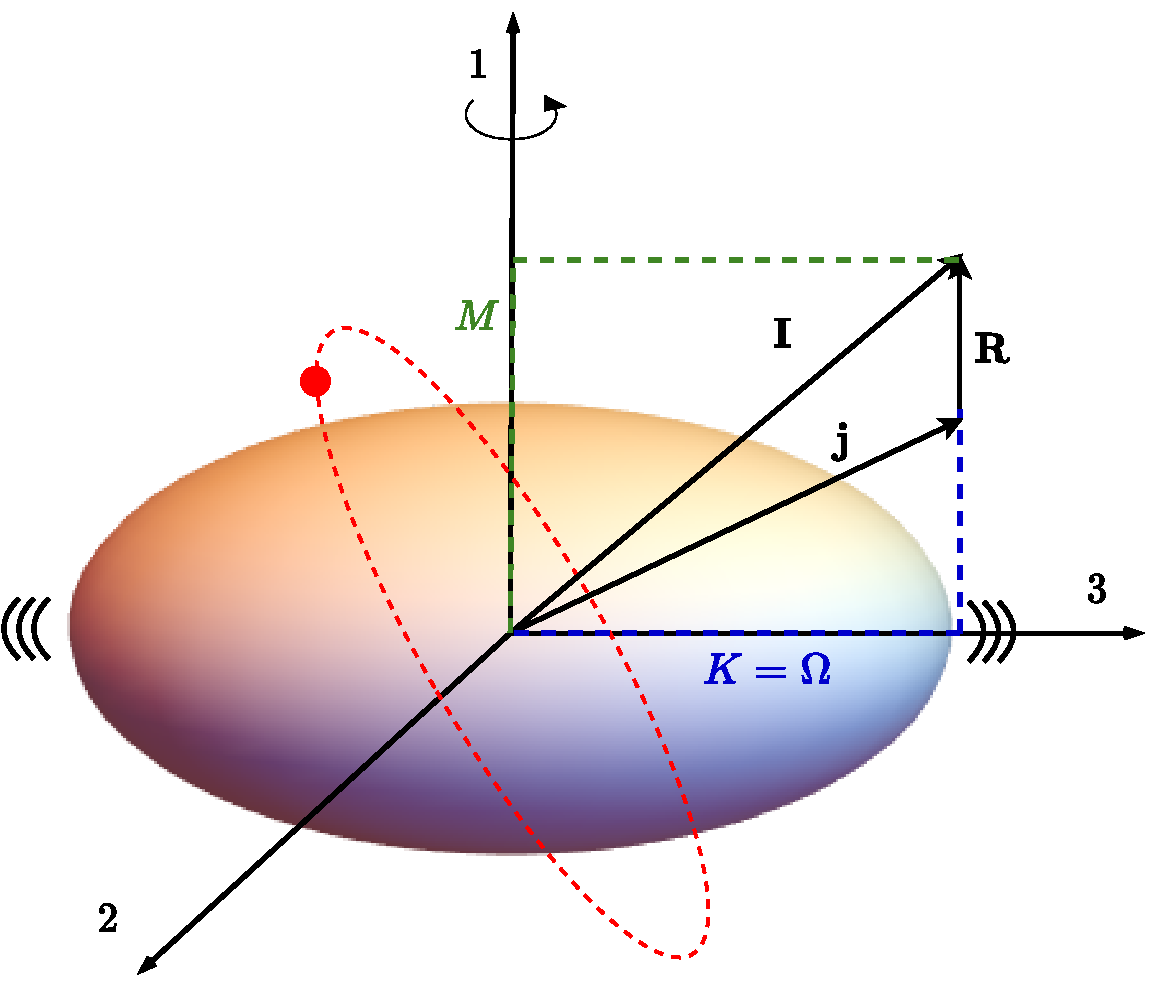
\includegraphics[scale=0.5]{Chapters/Figures/SCHEMATIC_COUPLING_ROTATIONAL.pdf}
    \caption{The coupling of the collective angular momentum with the angular momentum of a single-particle, for an axially deformed nucleus that is rotating about an axis perpendicular to the deformation axis.}
    \label{rotational-coupling-schematic}
\end{figure}

Based on the expression of $T_\text{rot}$ from Eq. \ref{kinetic-rotational-energy-collective}, its quantized form given in Eq. \ref{eq-rotational-energy-quantized}, and the coupling scheme depicted in Fig. \ref{rotational-coupling-schematic}, it is possible to construct a Hamiltonian that corresponds to rotating nucleus which has no valence particle. More precisely, the $\mathbf{j}$ term is neglected, such that only the pure collective motion of a nucleus is emphasized ($\mathbf{I}=\mathbf{R}$). This approximation is however only valid for even-even nuclei and for the low-lying states \cite{bertulani2007nuclear,davydov1958rotational}:
\begin{align}
    H&=H_\text{rot}+H_\text{intr}=\sum_i\frac{\hbar^2}{2\mathcal{I}_i}R_i^2\ ,
\end{align}
where the second term $H_\text{intr}$ represents some effects coming from the internal structure of the rotator itself. However, most of the time these terms can be neglected, leading to a rather simple energy spectrum for the even-even nuclei:
\begin{align}
    E_\text{rot}(I)=\frac{\hbar^2}{2\mathcal{I}_\perp}I(I+1)\ .
    \label{eq-simple-rotor-spectrum}
\end{align}

In the above expression, the MOI $\mathcal{I}_\perp$ corresponds to an axis that is perpendicular to the symmetry axis (i.e., either $1$-axis or the $1$-axis) of the ellipsoid. In the case of axial symmetry both moments are equivalent, such that the general notation $\mathcal{I}_\perp$ is made. As an observation, since there is no single-particle contribution, the quantized angular momentum $I$ (or spin) is equivalent to $R$. The spectrum defined by Eq. \ref{eq-simple-rotor-spectrum} leads to energy spacings $\propto I(I+1)$, which is also met in the  molecular spectra. The ground-state will always be the state $0^+$, and due to the mirror symmetry that is required for the wave-functions describing the even-even nuclei \cite{ring2004nuclear}, every other excited state will be represented by an even value of the spin: $2^+,4^+,\dots$.
The ratio $E(4^+)/E(2^+)$ for these bands is $3.33$ (as it was previously mentioned). This is indeed the best signature for the rotational phenomena in nuclei, indicating a clear presence of deformation + rotational motion. In a previous work by the current team (Raduta et al.) \cite{raduta2017semiclassical}, some spectra of even-even $^{158}$Er were studied and agreement with the observed experimental data was impressive. The energy spectra obtained from Eq. \ref{eq-simple-rotor-spectrum} has a classical counterpart which is known within literature as the \emph{symmetric top}. Fig \ref{rotational-bands-even-even} shows some examples of rotational bands in even mass nuclei, where the $K^pi=0^+$ band head is the ground-state, and every excited state has $\Delta I=2$ units of angular momentum.

\begin{figure}
    \centering
    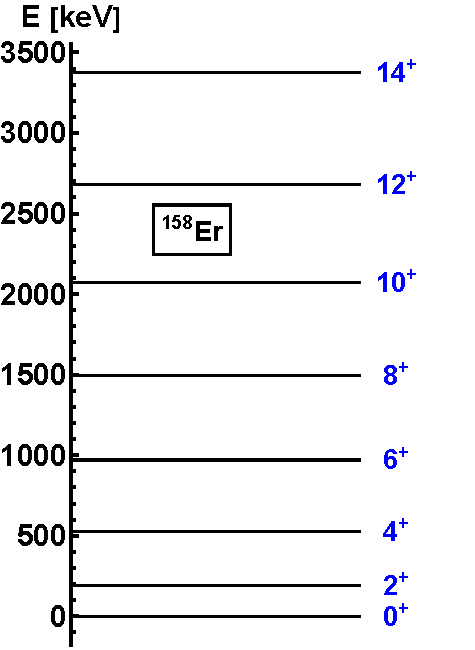
\includegraphics[scale=0.7]{Chapters/Figures/Er158-Rotational-Bands.pdf}
    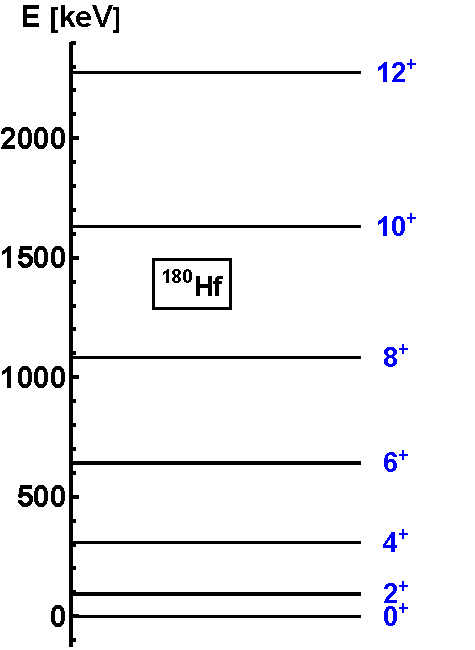
\includegraphics[scale=0.7]{Chapters/Figures/Hf180-Rotational-Bands.pdf}
    \caption{Experimental data showing the rotational bands in even-even nuclei. Note the spacing between the states that increases with $I$ via the rule from Eq. \ref{eq-simple-rotor-spectrum}. Experimental data are taken from Refs. \cite{nica2017nuclear,mccutchan2015nuclear} for each nucleus.}
    \label{rotational-bands-even-even}
\end{figure}

However, the spectra of a simple rigid rotator assumes that the projection $K$ of the total angular momentum for the ground-state of even-even nuclei is $K=0$. So the next step is to consider more general cases of nuclear rotation. There are two general cases of rotational bands that can occur, and both require the coupling scheme of a rotor with a valence nucleon, such that the angular momentum will be $\mathbf{I}=\mathbf{R}+\mathbf{j}$ (so both situations will correspond to odd-$A$ nuclei). The two situations are called \emph{Deformation aligned bands} and \emph{Rotation aligned bands} \cite{uwitonze2015assignment}. Graphical representation with both rotational schemes can be seen in Fig. \ref{ral-dal-coupling-bands}.

\begin{figure}
    \centering
    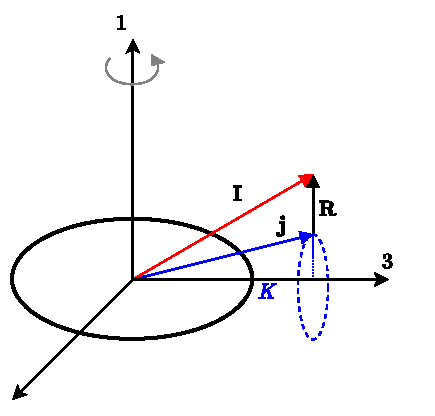
\includegraphics[scale=0.9]{Chapters/Figures/DAL_scheme.pdf}
    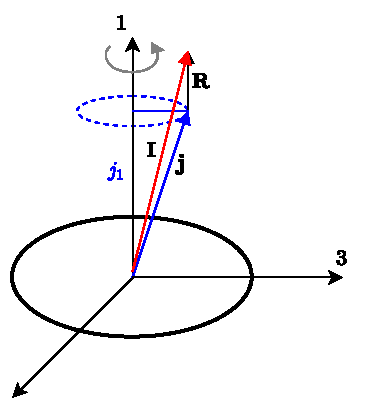
\includegraphics[scale=0.9]{Chapters/Figures/RAL_scheme.pdf}
    \caption{A sketch with the geometrical interpretation of the two ways a nucleus can exhibit rotational bands: Deformed Aligned Bands (\textbf{left}) and Rotation Aligned Bands (\textbf{right}). See text for explanations. The projections of the single-particle's total a.m. on the deformation and rotation axes are denoted with $K$ and $j_1$, respectively.}
    \label{ral-dal-coupling-bands}
\end{figure}

\subsubsection*{Deformation Aligned Bands}

This case is also referred to as \emph{strong-coupling} limit \cite{bohr1953collective} since the particle's a.m. is tightly coupled to the deformation axis (i.e., the symmetry axis). The general Hamiltonian will be:
\begin{align}
    H_\text{rot}=H_0+H_\text{coupl}\ ,
\end{align}
where $H_0$ is the already discussed operator containing the squared components $I_k$ of $\mathbf{I}$ and the extra \emph{coupling term} represents the Coriolis force \cite{bertulani2007nuclear}. The Coriolis effect is reflected by the coupling of the collective motion of the nucleus to the odd nucleon's motion. Despite that, it can be neglected at small rotations.

The projection of the particle's a.m. on the symmetry axis is a good quantum number, and if $\mathbf{R}$ is pointing in a direction that is perpendicular to the deformation axis, then $\Omega=K$, meaning that the energy spectrum will be given by:
\begin{align}
    E_\text{rot}(I)=\frac{\hbar^2}{2\mathcal{I}_\perp}\left[I(I+1)-K(K+1)\right]\ ,
\end{align}
or more formally:
\begin{align}
    E_\text{rot}(I)=\frac{\hbar^2}{2\mathcal{I}_\perp}\left[I(I+1)-K^2\right]+E_0(K)\ .
\end{align}
The rotational band will be constructed on the ground-state $E_0(K)$, where to total spin $I$ will be composed of a sequence $I=K,K+1,K+2,\dots$ and $K\neq\frac{1}{2}$. Consequently, this situation will lead to rotational bands where the difference between two consecutive states is only une unit of angular momentum. It should be pointed out that odd-$A$ nuclei can have multiple rotational bands that are built on different values of $K$.

For $K=\frac{1}{2}$, the band structure will follow:
\begin{align}
    E_\text{rot}(I)=\frac{\hbar^2}{2\mathcal{I}_\perp}\left[I(I+1)+a(-)^{I+\frac{1}{2}}(I+\frac{1}{2})\right]\ .
    \label{deformation-aligned-energy}
\end{align}

The nature of $(-1)^{I+1/2}$ will be explained for \emph{Rotation Aligned Bands}. Moreover, the term $a$ is called the \emph{decoupling parameter} \cite{bertulani2007nuclear}, and it can be determined from the first two experimental energy levels.  Experimental data which point out the presence of rotational bands with $K=1/2$ and $K\neq 1/2$ are shown in Fig. \ref{rotational-bands-odd-a}, for two odd-$A$ nuclei.

\begin{figure}
    \centering
    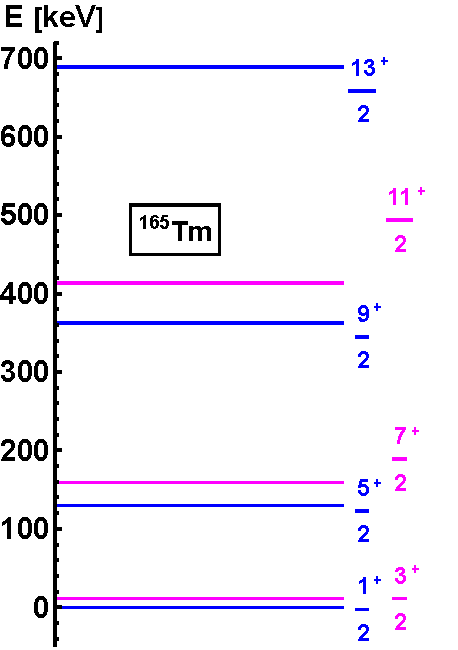
\includegraphics[scale=0.7]{Chapters/Figures/Tm165-Rotational-Bands.pdf}
    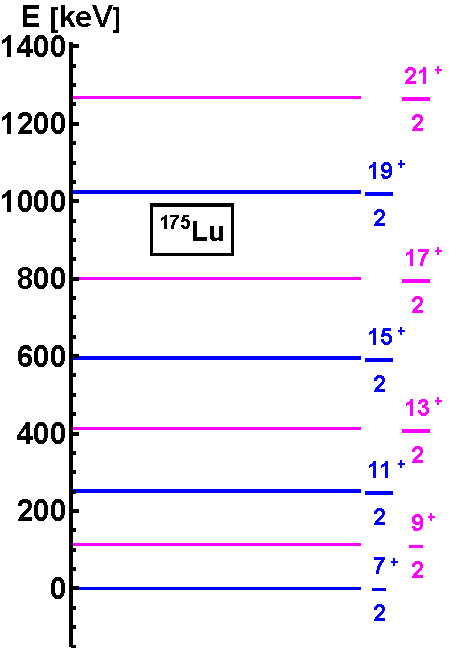
\includegraphics[scale=0.7]{Chapters/Figures/Lu175-Rotational-Bands.pdf}
    \caption{Rotational bands in odd-$A$ nuclei with the $K$ quantum number equal to $K=1/2$ (\textbf{left}) and $K\neq 1/2$ (\textbf{right}).}
    \label{rotational-bands-odd-a}
\end{figure}

\subsubsection*{Rotation Aligned Bands}

This situation is also called the \emph{decoupling limit} \cite{bohr1998nuclear} and it leads to the apparition of \emph{decoupled bands}. Here the total angular momentum is more aligned to the axis of rotation, and its maximum projection is along this axis. This is usually happening at high-spins, meaning strong rotational motion, which makes the angular momentum of the odd-particle to depart from the symmetry axis and align more and more with the direction of rotation (through the Coriolis effect). As such, the coupling term $H_\text{coupl}$ from $H_\text{rot}$ is not neglected here:
\begin{align}
    H_\text{rot}=\frac{\hbar^2}{2\mathcal{I}_\perp}\left(\mathbf{I}^2+\mathbf{j}^2-2\mathbf{I}\cdot\mathbf{j}\right)\ .
\end{align}

It is usually preferred to work with the \emph{raising} and \emph{lowering} operators which correspond to the angular momentum operator: $\mathbf{I}_\pm=\mathbf{I}_1\pm i \mathbf{I}_2$ (equivalently can be done for $\mathbf{j}$), bringing $H_\text{rot}$ to the following expression:
\begin{align}
    H_\text{rot}&=\frac{\hbar^2}{2\mathcal{I}_\perp}\hat{I}^2+\frac{\hbar^2}{2\mathcal{I}_\perp}\hat{j}^2-\frac{\hbar^2}{\mathcal{I}_\perp}K^2+H_\text{Coriolis}\ ,\\
    H_\text{Coriolis}&=-\frac{\hbar^2}{2\mathcal{I}_\perp}(\mathbf{I}_+\mathbf{j}_-+\mathbf{I}_-\mathbf{j}_+)\ .
\end{align}

It is worth pointing out that the effect of the Coriolis term is to couple bands which differ in $K$ quantum number with one unit, effect which is negligible at high deformations and low spins (since the single-particle motion is tightly bound to the bulk nucleus) while at very high rotations (spins) it becomes significant. Consequently, the Coriolis effect most probably occurs in prolate nuclei for an `almost empty' $j$-shells and oblate nuclei for an `almost full' $j$-shell.

When the single-particle angular momentum is orienting itself to the direction of rotation, the projection of $\mathbf{j}$ can be denoted by $j_1$ (keeping a consistency with Fig. \ref{rotational-coupling-schematic}). The spectrum of the decoupled bands will be:
\begin{align}
    E_\text{rot}(I)=\text{const.}+\frac{\hbar^2}{2\mathcal{I}_\perp}(I-j_1)(I-j_1+1)\ ,
\end{align}
where the coupling terms have been embedded in the constant term. This leads to a spin sequence $I=j_1,j_1+2,j_1+4\cdots$, which differs from the previous case via the constant $2\hbar$ angular momentum difference of two consecutive levels.

In order to understand the terms $(-1)^{I+1/2}$ from Eq. \ref{deformation-aligned-energy}, it is required to describe the wave-function corresponding to the particle-core system. Indeed, using the specific quantum numbers $I,K,M$ with their meaning explained in Fig. \ref{rotational-coupling-schematic}, the wave-function will be written as a combination of rotational (the Wigner $D_{MK}^I$ functions) and single-particle components \cite{wang2007exotic,davydov1958rotational}:
\begin{align}
    \Psi_{MK}^I=\ket{IMK}=N\left[\phi_K D_{MK}^I+(-)^{I+K}\phi_{-K}D_{M-K}^I\right]\ ,
\end{align}
where $N$ is the normalization constant, usually having the value $N_I=\sqrt{\frac{2I+1}{16\pi^2}}$. This linear combination of states with $K$ and $-K$ induces a degeneracy and it is due to the invariance of such a system with respect to rotations by $\pi$ around the rotational axis \cite{frauendorf1997tilted,bohr1998nuclear}. The factor $(-)^{I+K}\equiv\alpha$ is called the \emph{signature} and it reflects wether a system is invariant or not to such a rotation. More precisely, the \emph{signature quantum number} is given as \cite{sun1994varied}:
\begin{align}
    \alpha_I=\frac{1}{2}(-)^{I-\frac{1}{2}}\ ,
\end{align}
for a state of spin $I$ in an odd-$A$ nucleus, resulting in the favored states having $\alpha_\textbf{favored}=\frac{1}{2}$ and the unfavored states having $\alpha_\text{unfavored}=-\frac{1}{2}$.

Depending on the signature, the nuclear states can be divided into two sets: one that follows $I=K,K+2,K+4,\dots$ and $I=K+1,K+3,K+5,\dots$. This is the reason why for the decoupled bands, one can regard them as an `initial' rotational band $I,I+1,\dots$ that is `broken' apart in two sequences: one that is favored and one that is unfavored (opposite signature).
An example is a nucleus with odd-$A$, where the favored bands have spins $I_\text{favored}=\frac{1}{2},\frac{5}{2},\frac{1}{2},\dots$, while their unfavored \emph{partner} bands have spins $I_\text{unfavored}=\frac{3}{2},\frac{7}{2},\frac{11}{2},\dots$ and opposite signature (also known as \emph{signature partners}). In fact, taking a closer look at the rotational bands specific to odd-$A$ nuclei shown in Fig. \ref{rotational-bands-odd-a}, each consecutive level is a state with different signature, meaning that each `group' of colors classifies into a set of favored (blue) and unfavored (magenta) states.

This divided set of partner bands also has some characteristics that can be observed throughout experimental measurements. Firstly, the splitting of the two branches implies that the favored states will generally have lower excitation energy than their unfavored partners. This is also proved by the expression of the rotor energy given in Eq. \ref{deformation-aligned-energy}, where the decoupling parameter will cause an upward (downward) shift in energy for states with $I=1/2,5/2,9/2,\dots$ ($I=3/2,7/2,11/2,\dots$), depending whether $a$ is positive (negative). The experimental data shown in Fig. \ref{level-scheme-signature-splitting} shows how the favored partner lies lower with respect to its unfavored partner bands, each having the corresponding spin sequence $\Delta I=2$ for intraband states and $\Delta I=1$ for interband states. Such spectra are very often met in the decay schemes for odd-mass nuclei in which the rotational motion is governed by the (core+particle) coupling scheme.
\begin{figure}
    \centering
    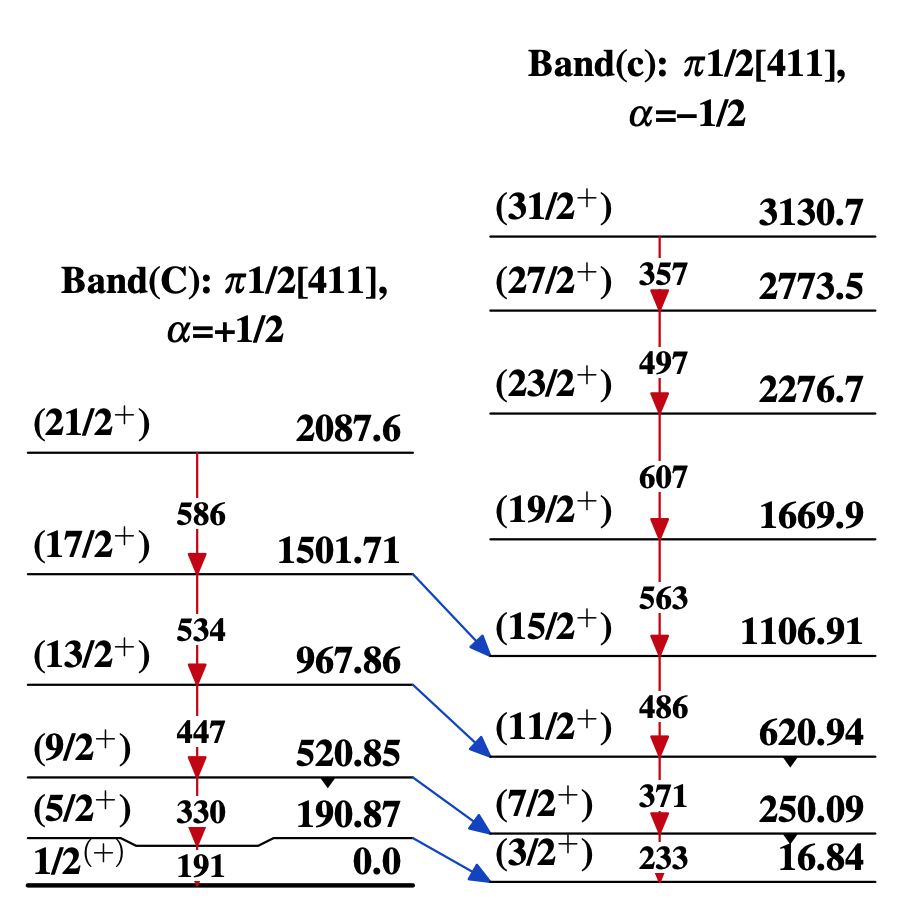
\includegraphics[scale=0.45]{Chapters/Figures/Lu_163_K12-band.png}
    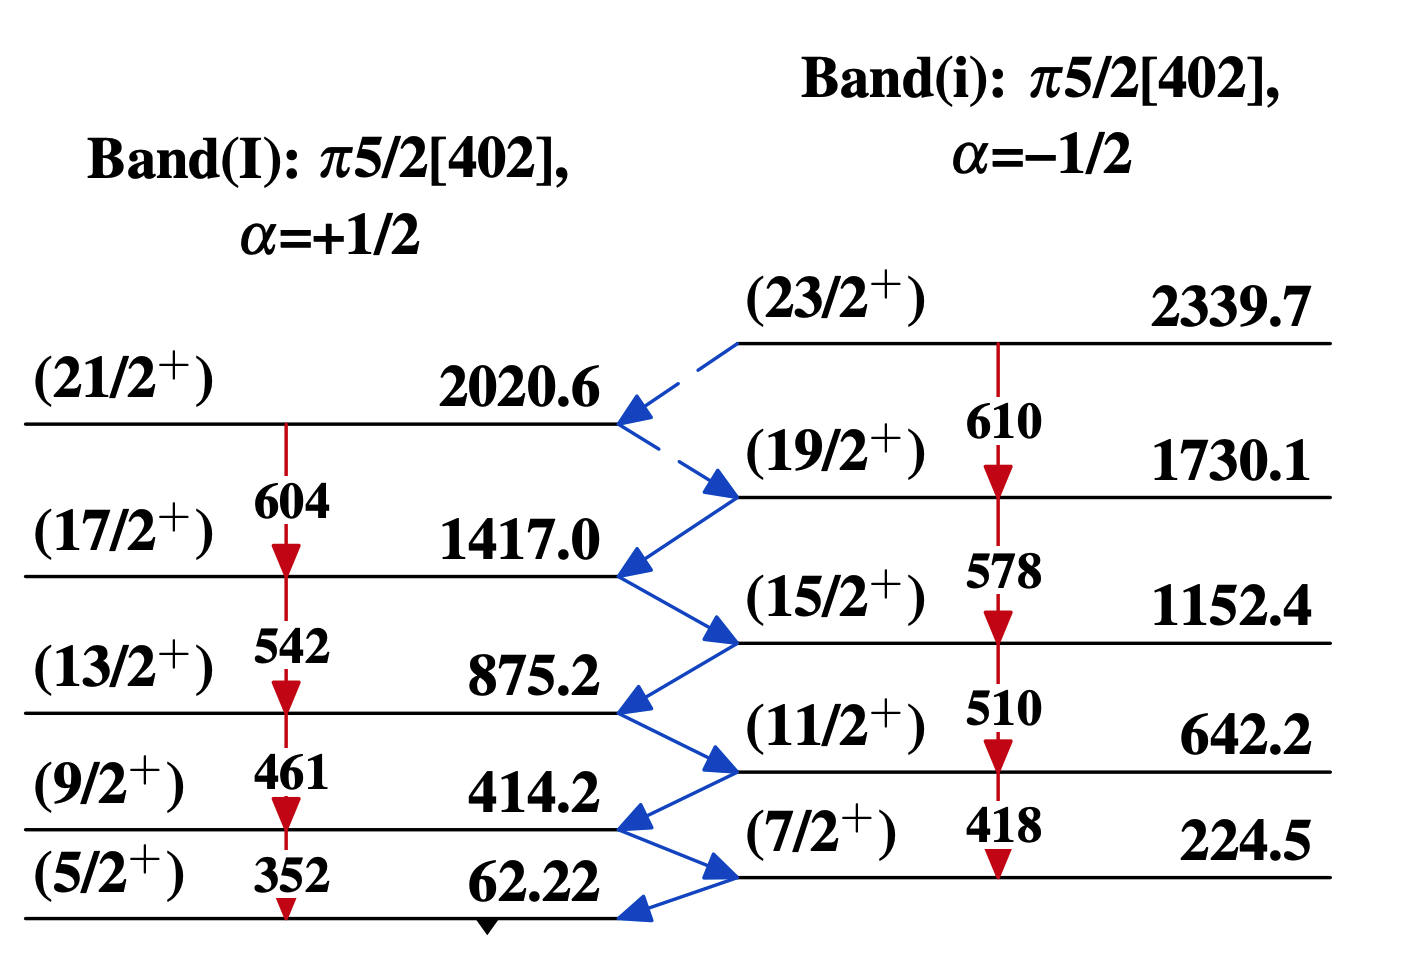
\includegraphics[scale=0.28]{Chapters/Figures/Lu_163_signatureSplitting.png}
    \caption{Experimental level schemes for $^{163}$Lu showing pairs of signature partner bands. \textbf{Left}: the two bands are built on a proton with $j=1/2$ and positive parity. \textbf{Right}: sequences built on a proton with $j=5/2$ with the same parity. The Nilsson quantum numbers are defined for each band. Note the spin difference between each state, as described in text. Also note the lower energies for the favored states. Interband transitions are marked with the blue arrows. These figures were taken from Ref. \cite{reich2010nuclear}.}
    \label{level-scheme-signature-splitting}
\end{figure}

\subsection{Superimposed Rotations and Vibrations}

Up until now, the two types of nuclear motion, namely the collective rotations and vibrations were discussed separately. The small vibrations of the nuclear surface lead to the presence of band structures constructed via the quadrupole phonons carrying $\lambda=2$ units of angular momentum. The collective nature of the nucleus together with effects coming from the coupling a core to a valence nucleon also showed that some rotational band structures can appear in nuclei.

The proper picture of a rotating deformed nucleus consists of a stable \emph{equilibrium shape} that is determined by the \emph{rapid internal motion of the nucleons} within the nuclear potential and their entire distribution doing a \emph{slow rotation}, such that it has negligible effect on the nuclear structure or on the individual nucleonic orbits.

Besides the two (separated) degrees of freedom for the nuclear system (i.e., collective rotation and vibrations), the two types of motion can be superimposed on each other, leading to specific spectra of the nuclei. One can describe this spectra starting from the expression of the \emph{Collective Bohr's Hamiltonian} (remember calculations presented in Eqs. \ref{collective-hamiltonian-stiffness-inertia}, \ref{bohr-collective-potential}, \ref{kinetic-vibrational-energy-collective}, and \ref{kinetic-rotational-energy-collective}):
\begin{align}
    H_\text{coll}=T+V=T_\text{vib}+T_\text{rot}+V
\end{align}

Following the calculations from \cite{li2022model}, a separation of the Hamiltonian terms in three main components will be made: one associated to the rotation of a rigid rotor characterized by a total spin and well-defined MOI, one associated to the $\beta$-vibration, and the last corresponds to the $\gamma$-vibrational mode. The total energy forms the final spectrum \cite{ring2004nuclear,li2022model}:
\begin{align}
    E_{n_\beta n_\gamma IK}=\hbar\omega_\beta\left(n_\beta+\frac{1}{2}\right)+\hbar\omega_\gamma\left(n'_\gamma+\frac{1}{2}|K|\right)+\frac{\hbar^2}{2\mathcal{I}}\left[I(I+1)-K^2\right]\ .
    \label{collective-rotation-vibration-energy-spectrum}
\end{align}
Note the two harmonic-like solutions making the vibrational mode present within the energy formula. The two `frequencies' are given in terms of the stiffness and inertia parameters \cite{li2022model}:
\begin{align}
\omega_\beta=\sqrt{\frac{C_0}{B_2}}\ ,\ \omega_\gamma=\sqrt{\frac{C2}{B_2}}\ ,   
\end{align}
and the two quantum numbers are as follows: 
\begin{align}
    n_\beta=0,1,\dots\ ,\ n'_\gamma=2n_\gamma+1\ ,\ n_\gamma=0,1,\dots\ .
\end{align}

The allowed values for the quantum numbers are as:
\begin{align}
    K&=0,2,4,\dots\ ,\nonumber\\
    I&=\begin{cases}
        K,K+1,K+2,\dots &\text{for} K\neq 0\\
        0,2,4,\dots &\text{for} K=0\\
   \end{cases}\ .
\end{align}

Consequently, the spectrum of a typical nucleus in which both vibration and rotation occurs has bands that are characterized by the set of quantum numbers $K,n_\beta,n_\gamma$, where the excited states follow the $\propto I(I+1)$ rule. The main bands are:
\begin{enumerate}
    \item the ground-state band, having states with even $I$, where excitation energies are constructed from the rotor term
    \item the $\beta$ band, starting above the g.s. band with $\hbar\omega_\beta$ and containing only even spins
    \item the $\gamma$ band, corresponding to $K=2$ (as explained in a previous section). It is distinguished from the $\beta$ band because it starts with $2^+$ as first state and it contains both odd and even spins.
    \item the higher-level bands are the $n_\gamma=1$ and $K=4$ bands for $\gamma$-vibrational mode, and the $\beta$ band with $n_\beta=2$.
\end{enumerate}
This collective spectrum is exemplified in Fig. \ref{collective-rotation-vibration-energy-levels}

\subsection{Collective Quantities}

In this section, some important quantities will be described since their meaning is strictly related to the collective nature of nuclei. Indeed, one can understand nuclear deformation, energy spectra, and behavior with respect to spin of nuclei by studying quantities such as \emph{rotational frequencies}, \emph{moments of inertia}, \emph{quadrupole moments}, and so on. As it will be shown, the values of such physical observables will point out, for example, if some nuclei experience large deformations, or if rotation causes the nucleus to exhibit excited states. Moreover, the comparison with experimental data for these quantities can help validate some assertions that are initially made, which is usually the crucial test of new models and frameworks that are developed by the nuclear physics community.

\subsubsection*{R - Energy ratio}

As discussed before, the energy ratio between the first excited $4^+$ state to the first excited $2^+$ state is a very good test for checking wether a nucleus `tends' to show rotational or vibrational structures (i.e., spectra). Casten et al. \cite{casten2000nuclear} shows the evolution of this ratio across the mass number $A$, and a classification between \emph{vibrational} vs. \emph{rotational} character can be made. Fig. \ref{4state-2state-ratio} contains the ratio $R_{4^+/2^+}$.

\begin{figure}
    \centering
    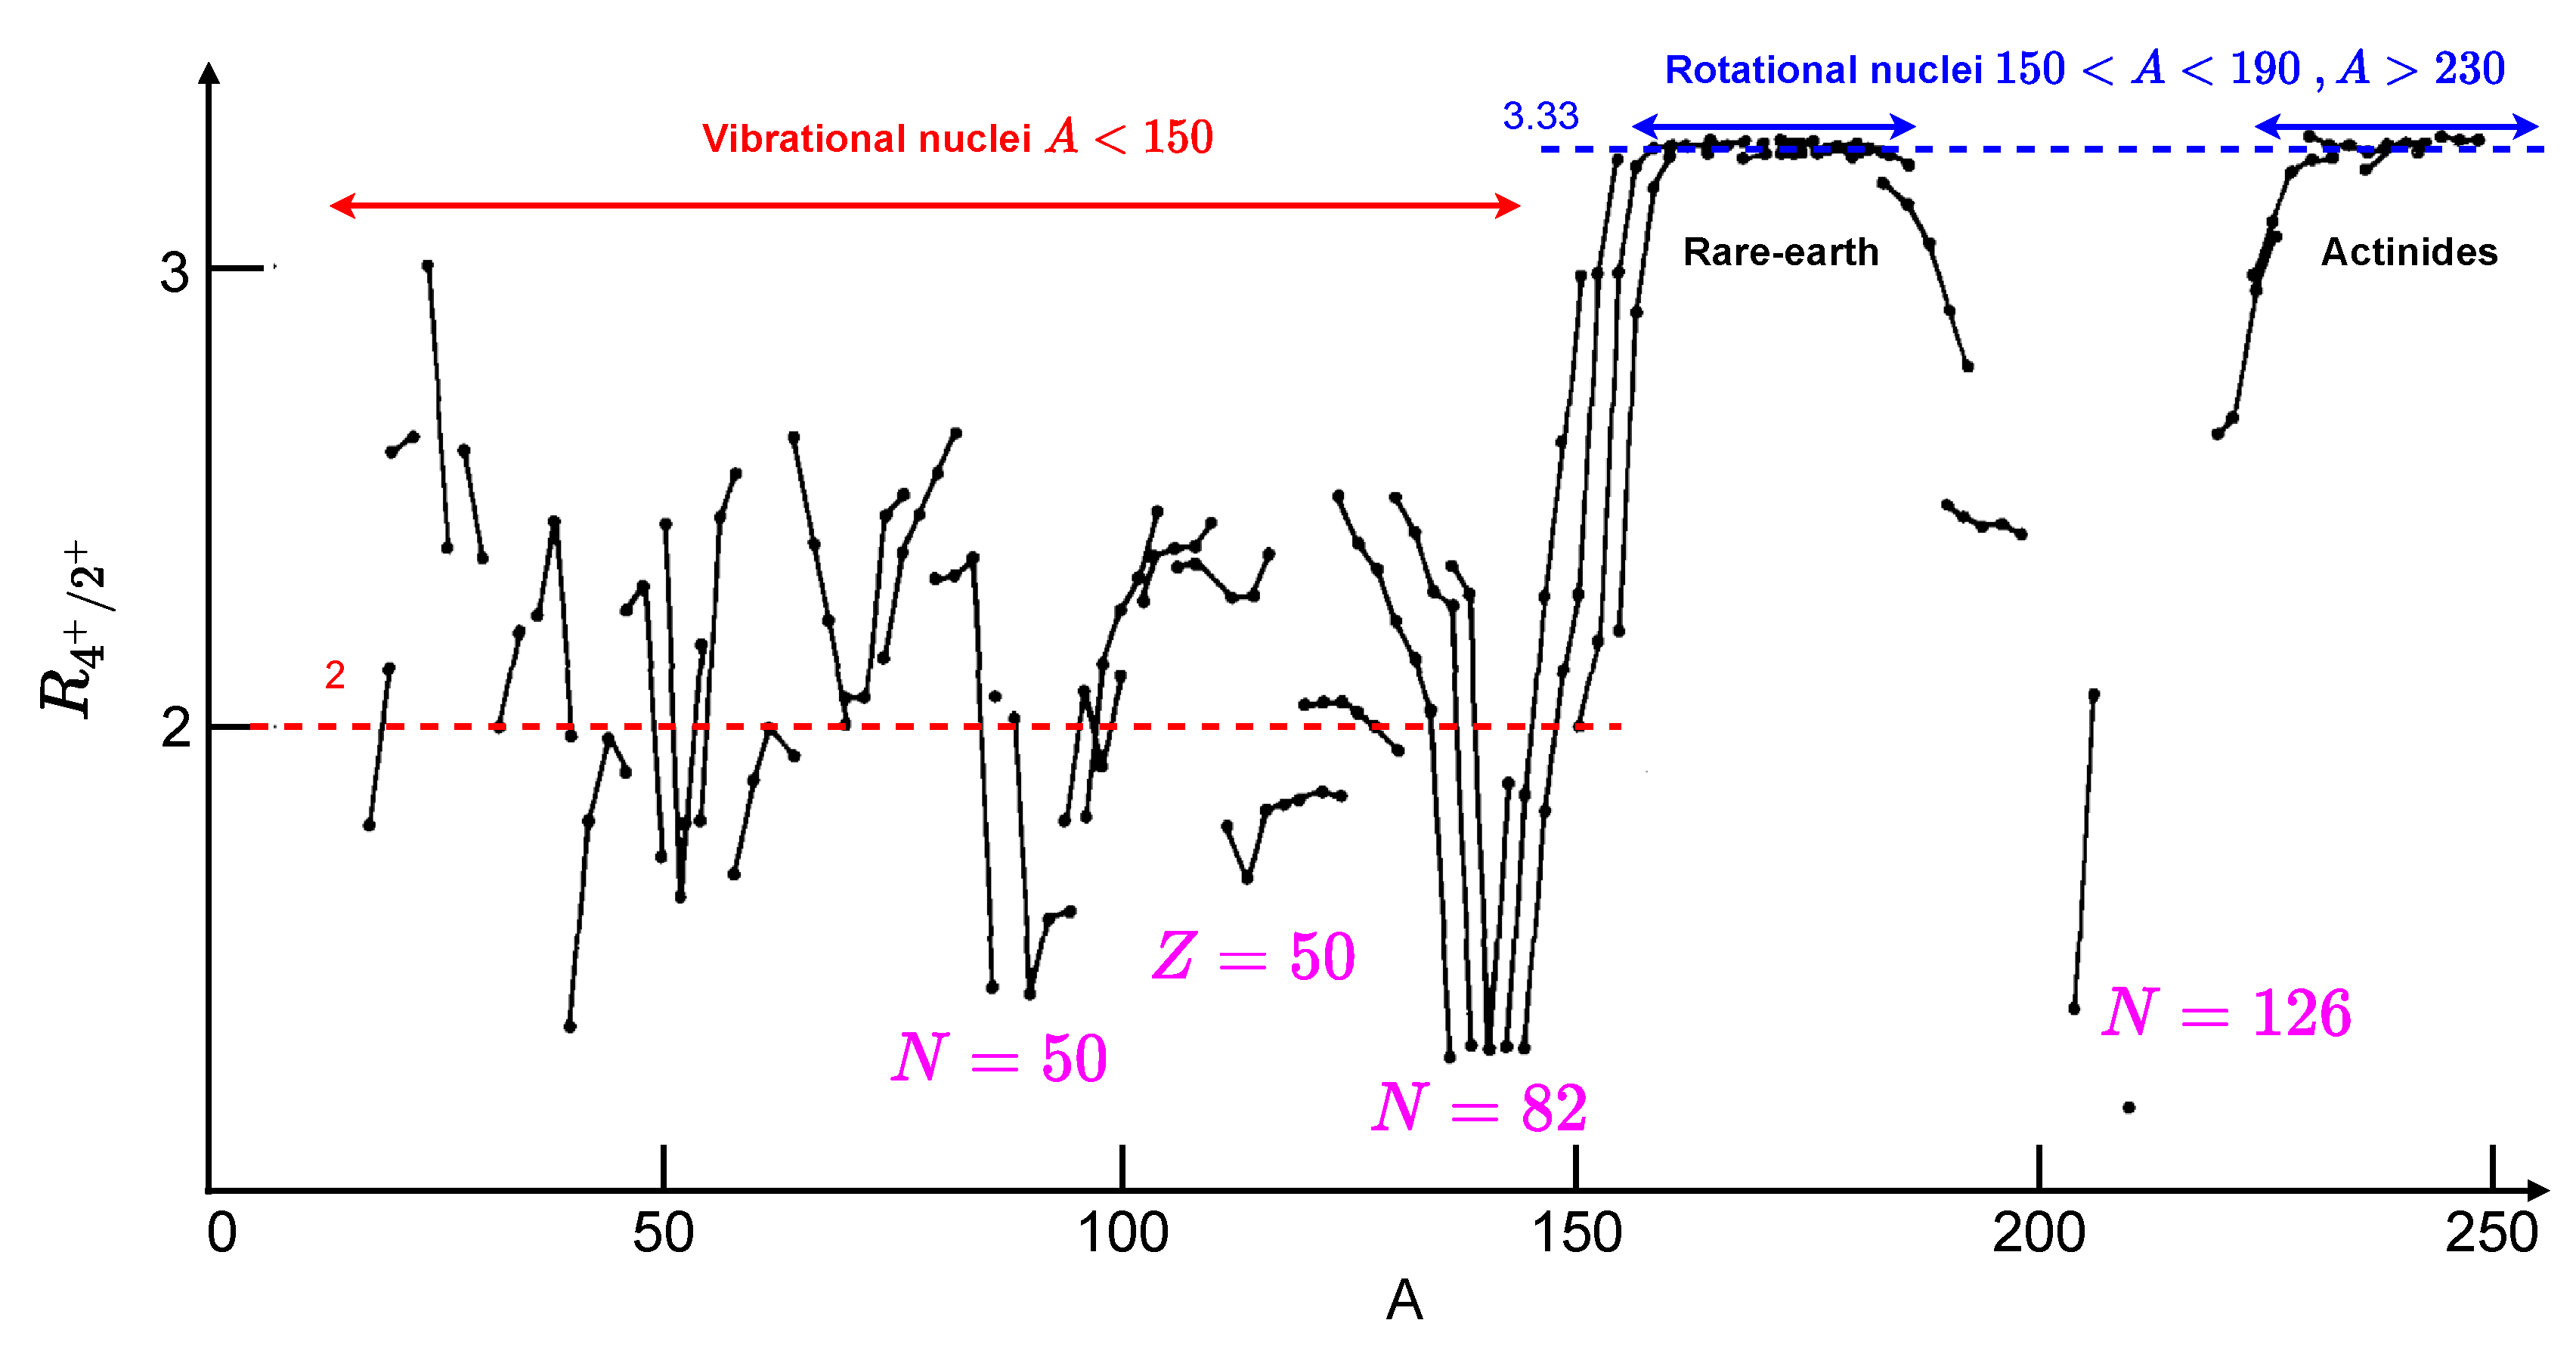
\includegraphics[scale=0.251]{Chapters/Figures/vibrations_rotations_E42-ratio.pdf}
    \caption{The experimental ratio $R_{4^+/2^+}$ in even-$Z$ and even-$N$ nuclei. Each line is connecting sequences of isotopes. Note the two important values for $R_{4^+/2^+}$, namely $2$ and $3.33$ given for a perfect vibrational nucleus and a pure rotator, respectively. Text with magenta color marks the magic numbers for $Z$ or $N$. This plot was adapted from Ref. \cite{casten2000nuclear}.}
    \label{4state-2state-ratio}
\end{figure}

\subsubsection*{Rotational frequencies}

The kinetic energy of a rotating object, in the classical limit, is described as a quadratic variation of the angular frequency (frequency of rotation around a particular direction) $\omega=l_\text{cls.}/\mathcal{I}$ in the following way:
\begin{align}
    E=\frac{1}{2}\mathcal{I}\omega^2\ ,
\end{align}
which can also be given in terms of the angular momentum $l_\text{cls.}$, such that the final energy becomes $E_\text{cls.}=l_\text{cls.}^2/(2\mathcal{I})$. Quantum mechanically, it was shown that $l^2$ is usually expressed as $\hat{l}^2_\text{quantum}=\hbar^2 I(I+1)$.

Bengtsson et al. \cite{bengtsson1979quasiparticle} calculated the so-called Routhians (single-particle energies within the rotating frame of reference) and they found a \emph {canonical relation} between the energies and rotational frequencies:
\begin{align}
    \omega=\frac{\text{d}E(I)}{\text{d}I_x}\ ,
\end{align}
where the term $I_x$ is called the \emph{aligned angular momentum}, and usually it denotes the experimental spin of every state minus a reference value (see Harris \cite{harris1965higher}). The signature property discussed previously (giving sequences with $\Delta I=2$) plays a pivotal role in determining $I_x(I)$, since the projection $K$ of the angular momentum onto the deformation axis must be taken into account:
\begin{align}
    I_x(I)=\sqrt{\left(I+\frac{1}{2}\right)^2-K^2}\ ,
    \label{aligned-angular-momentum}
\end{align}
which for the $K=0$ bands reaches the simplified form $I_x^2=(I+\frac{1}{2})^2$. The value of $K$ is typically the band-head's angular momentum \cite{bengtsson1979quasiparticle,bengtsson1984signature}. 

A more concise definition for the quantity $\omega(I)$ is related to the transition between two consecutive states $I+1\to I-1$ within a rotational band: a unique value of $\omega$ is attributed to the spin $I$, which is defined as a mean value of the two angular momenta from the corresponding transition. Such a construction will yield a set of discrete points $\omega(I)$, and one can obtain a `continuous' function $\omega(I)$ together with its inverse $I(\omega)$, thus making the term $I$ from Eq. \ref{aligned-angular-momentum} to be in fact $I(\omega)$.

The rotational frequency is used to represent many quantities which characterize collective motion and nuclear deformation. For example, representing the total angular momentum $I$ (or the aligned one $I_x$) as a function of $\Omega$ can check wether multiple bands have the same nature. Moreover, as it will be shown in the following section, representing the MOI as function of $\omega$ will also get an insight on the intrinsic structure of the nucleus and the coupling schemes involved in the occurrence of the excited spectra. Another interesting feature that is present in high-spin spectra of some nuclei is the so-called \emph{backbending} phenomena, where due to the Coriolis effect, nucleons can suffer a de-pairing, leading to their angular momentum to orient along the rotational axis, thus leading to a sharp increase in the MOI \cite{ring2004nuclear,kvasil2004backbending}. These kind of effects are correlated to high deformation, increased rotation, and change in the nucleonic alignment.

\subsubsection*{Moments of inertia}

This is a crucial quantity which describes the degree of deformation for the nucleus (rotational ellipsoid), since the asymmetry between the three MOI dictates the shape of the nuclear matter (remember discussion from Chapter \ref{chapter-2}). It was already mentioned that it is possible to retrieve an \emph{experimental} value for a moment of inertia by inferring the energy spacing between consecutive levels of a collective spectrum. A classification of types of MOI was done in Eq. \ref{eq-irrotational-rigid-mois}, where the dependence of $\mathcal{I}$ on the deformation parameters (and even the mass parameter $B_\lambda$ that originates from the initial Bohr Hamiltonian \ref{collective-hamiltonian-stiffness-inertia}) was shown.

In order to get values for MOIs from the experimental data, two quantities are required: the spins and energies of two consecutive levels within an excited spectrum. The most general expression for the MOI can be written as \cite{ahmad2021backbending}:
\begin{align}
    \mathcal{I}=\frac{\hbar^2}{2}\left(\frac{\text{d}E}{\text{d}J(J+1)}\right)^{-1}\ ,
\end{align}
where the classical angular momentum $J$ is related to its quantum equivalent via the correction $J=I+1/2$ (see Eq. \ref{aligned-angular-momentum}). Practically, the derivative can be expressed in terms of the aligned angular momentum $I_x$ defined above.

Moreover, there are two types of MOI which give information about the structure of nuclei with respect to spin: \emph{kinematic MOI} and \emph{dynamic MOI}. The kinematic MOI is given by \cite{wu1992relation}:
\begin{align}
    \mathcal{I}^{(1)}=\frac{\hbar I_x}{\omega}=\hbar^2 I_x\left(\frac{\text{d}E}{\text{d}I_x}\right)^{-1}\ .
    \label{kinematic-moi-general}
\end{align}

One can see why the aligned angular momentum is important, since its variation w.r.t. the energies lead to theoretical determinations of the kinematic MOI. From the observed intraband $E2$ transitions one can extract the (kinematic) moment of inertia via the rule:
\begin{align}
    \mathcal{I}^{(1)}(I-1)=\hbar^2\frac{2I-1}{E_\gamma(I,I-2)}\ ,
    \label{kinematic-moi-energy-levels}
\end{align}
where $E_\gamma(I,I-2)$ represents the energy difference between two consecutive levels $E(I)$ and $E(I-2)$. The dependence on $I$ for this type of MOI makes its experimental determination to require some spin assignments to each state of the excited spectrum. On the other hand, the dynamic moment of inertia is expressed as \cite{wu1992relation}:
\begin{align}
    \mathcal{I}^{(2)}(I)=\hbar\frac{\text{d}I_x}{\text{d}\omega}=\hbar^2\left(\frac{\text{d}^2E}{\text{d}I_x^2}\right)^{-1}\ ,
    \label{dynamic-moi-general}
\end{align}
while $\mathcal{I}^{(2)}$ expressed in terms of the energy differences has the following form:
\begin{align}
    \mathcal{I}^{(2)}(I)=\hbar^2\frac{4}{\Delta E_\gamma(I)}=\hbar^2\frac{4}{E_\gamma(I+2,I)-E_\gamma(I,I-2)}\ .
    \label{dynamic-moi-energy-levels}
\end{align}
Note that any calculations for the dynamical MOI does not require prior knowledge about the spin assignments of the energy states. These two types of MOI are usually represented as function of the rotational frequency $\omega$. Since the total spin $I$ can be expressed as a function of rotational frequency, plotting the kinematic/dynamic MOI as function of angular momentum is also preferred. In the present work, these quantities are of high interest (graphical representations for different nuclei will be shown in a future chapter), their relative behavior will help characterize bands with similar nucleonic structure.

An alternative description of the quantitative analysis of these MOI can be done through the so-called $ab$ formula \cite{wu1992relation,wu1992spin}, where the energies corresponding to the rotational spectrum are parametrized as: $E(I)=a\left(\sqrt{1+bI(I+1)}-1\right)$. Fitting the experimental data will produce a set of parameters $(a,b)$ that will be used to get expressions for the kinematic and dynamic MOI:
\begin{align}
    \mathcal{I}^{(1)}=\mathcal{I}_0\left[1-\frac{(\hbar\omega)^2}{a^2b}\right]^{-1/2}\ ,\\
    \mathcal{I}^{(2)}=\mathcal{I}_0\left[1-\frac{(\hbar\omega)^2}{a^2b}\right]^{-3/2}\ ,
\end{align}
with the factor $\mathcal{I}_0$ defined as the \emph{band-head} moment of inertia: $\mathcal{I}_0=\frac{\hbar^2}{ab}$. In fact, such an approach of determining the MOIs of several odd-$A$ nuclei will consist in a future work of the same team.

As mentioned, the sharp or abrupt irregularities of the MOI with respect to the increase in rotational frequency is known as backbending. The Figs. \ref{fig-hfNuclei-mois}-\ref{fig-ErYbnuclei-mois} show some experimental data in which the quantity $\frac{2\mathcal{I}}{\hbar^2}$ as function of the squared rotational frequency is graphically represented.

\begin{figure}
    \centering
    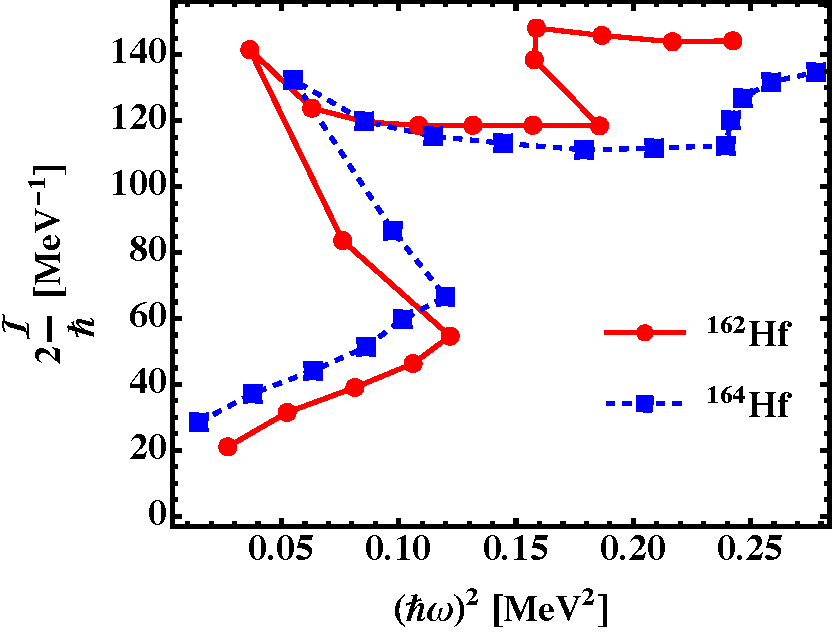
\includegraphics[scale=0.51]{Chapters/Figures/mois_Hf162-164.pdf}
    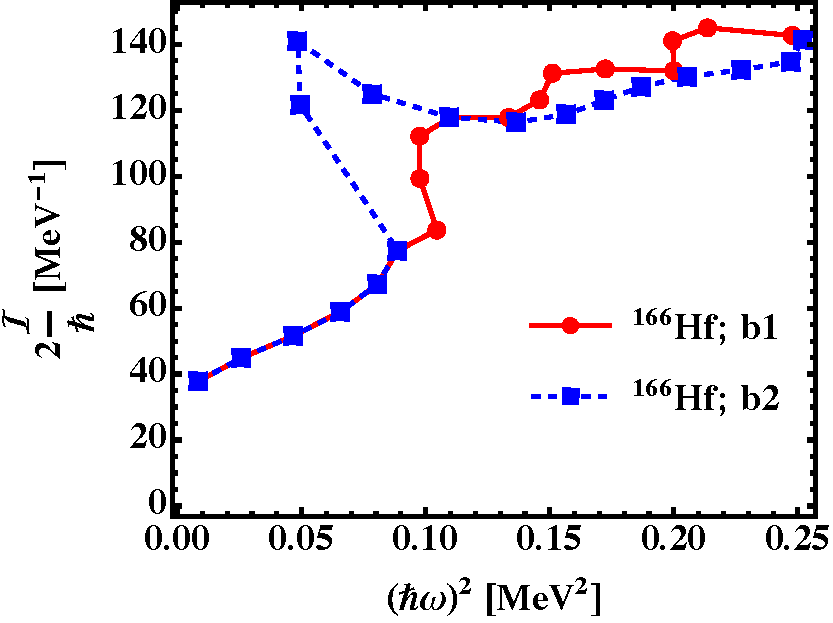
\includegraphics[scale=0.52]{Chapters/Figures/mois_Hf166.pdf}
    \caption{The moment of inertia as a function of rotational frequencies for three even-even nuclei. \textbf{Left:} The MOI for $^{162,164}$Hf nuclei, with their corresponding rotational ground-state bands. \textbf{Right:} The MOI for the first two rotational bands in $^{166}$Hf. Experimental data for these two nuclei are taken from Ahmad et al. \cite{ahmad2021backbending}.}
    \label{fig-hfNuclei-mois}
\end{figure}

\begin{figure}
    \centering
    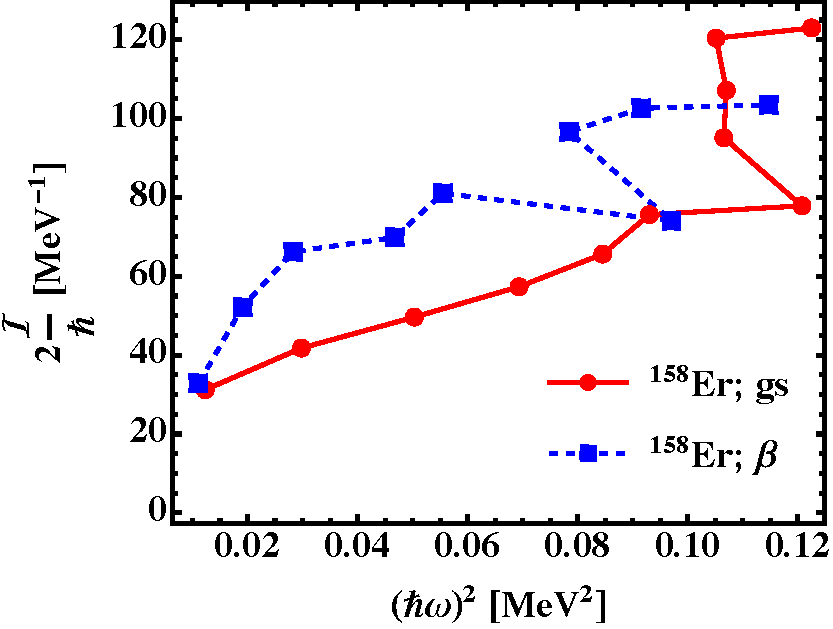
\includegraphics[scale=0.5]{Chapters/Figures/mois_Er158.pdf}
    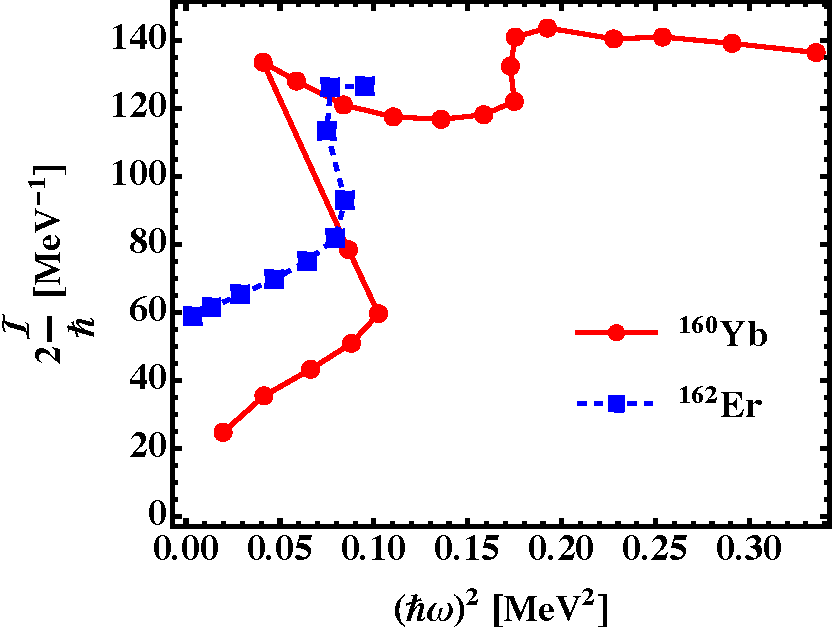
\includegraphics[scale=0.5]{Chapters/Figures/mois_Yb160Er182.pdf}
    \caption{\textbf{Left:} The MOI for $^{158}$Er nucleus, with the ground-state band $K^\pi=0^+$ and the $\beta$-vibrational band with the same quantum numbers. Experimental data taken from \cite{nica2017nuclear}. \textbf{Right:} The MOI for $^{160}$Yb compared with $^{162}$Er. Experimental data taken from \cite{nica2021nuclear} ($A=158$) and \cite{reich2007nuclear} ($A=162$).}
    \label{fig-ErYbnuclei-mois}
\end{figure}

Indeed, by looking at the evolution of $\mathcal{I}$, some sharp increases are noted, and usually these are attributed to the centrifugal stretching in the rotational model \cite{davydov1960rotation}. Moreover, the constant increase in $\mathcal{I}$ is considered to happen due to the slow and constant quenching of the pairing correlations between nucleons (as already discussed in terms of the Coriolis effect at high spin) \cite{mottelson1960effect}. The abrupt changes are explained as rapid phase transitions of the nucleonic matter \cite{krumlinde1974effect} exclusively due to the Coriolis Anti Pairing effect (example for some even-even nuclei in Ref. \cite{raduta2011semimicroscopic}).

\subsubsection*{Electric Quadrupole Moment}

One of the most important indicators of stable nuclear deformation is a large value for the \emph{electric quadrupole moment} \cite{hamamoto2016interplay}. The most general expression for the intrinsic quadrupole moment of a nucleus which is rotating about its $z$-axis is given in terms of its \emph{charge density distribution}:
\begin{align}
    Q_0=\int(3z^2-r^2)\rho(r)_\text{charge}\text{d}v\ .
\end{align}
This shows how the nuclear charge distribution inside the nucleus is a crucial indicator of deformations. Note this $z$ notation for a rotating axis is used here just for consistency with the textbook expression of $Q_0$ \cite{casten2000nuclear}. Indeed, a relationship between the deformation parameter $\beta$ and the quadrupole moment itself can be approximated (in second order of $\beta$) as:
\begin{align}
    Q_0=\frac{3}{\sqrt{5\pi}}R^2Z\beta(1+0.16\beta)\ ,
\end{align}
where $R$ is given as $R=R_0A^{1/3}$. For the $\beta$ values that correspond to proper deformed nuclei (i.e., $\beta\approx 0.3$), higher order terms are not necessary. Remember that $\beta$ describes the eccentricity of the deformed ellipsoid (albeit prolate or oblate), while the difference between prolate and oblate shapes is that for prolate (oblate) case there is an extension in one (two) direction and a squeezing in the other two (one). Depending on the value of $\beta$, the quadrupole moments for nuclei will be positive (indicating a stable prolate deformation) and negative (for stable oblate deformations). Fig. \ref{fig-quadrupole-beta-nuclides} shows some experimental values for some nuclei within the rare earth region.
\begin{figure}
    \centering
    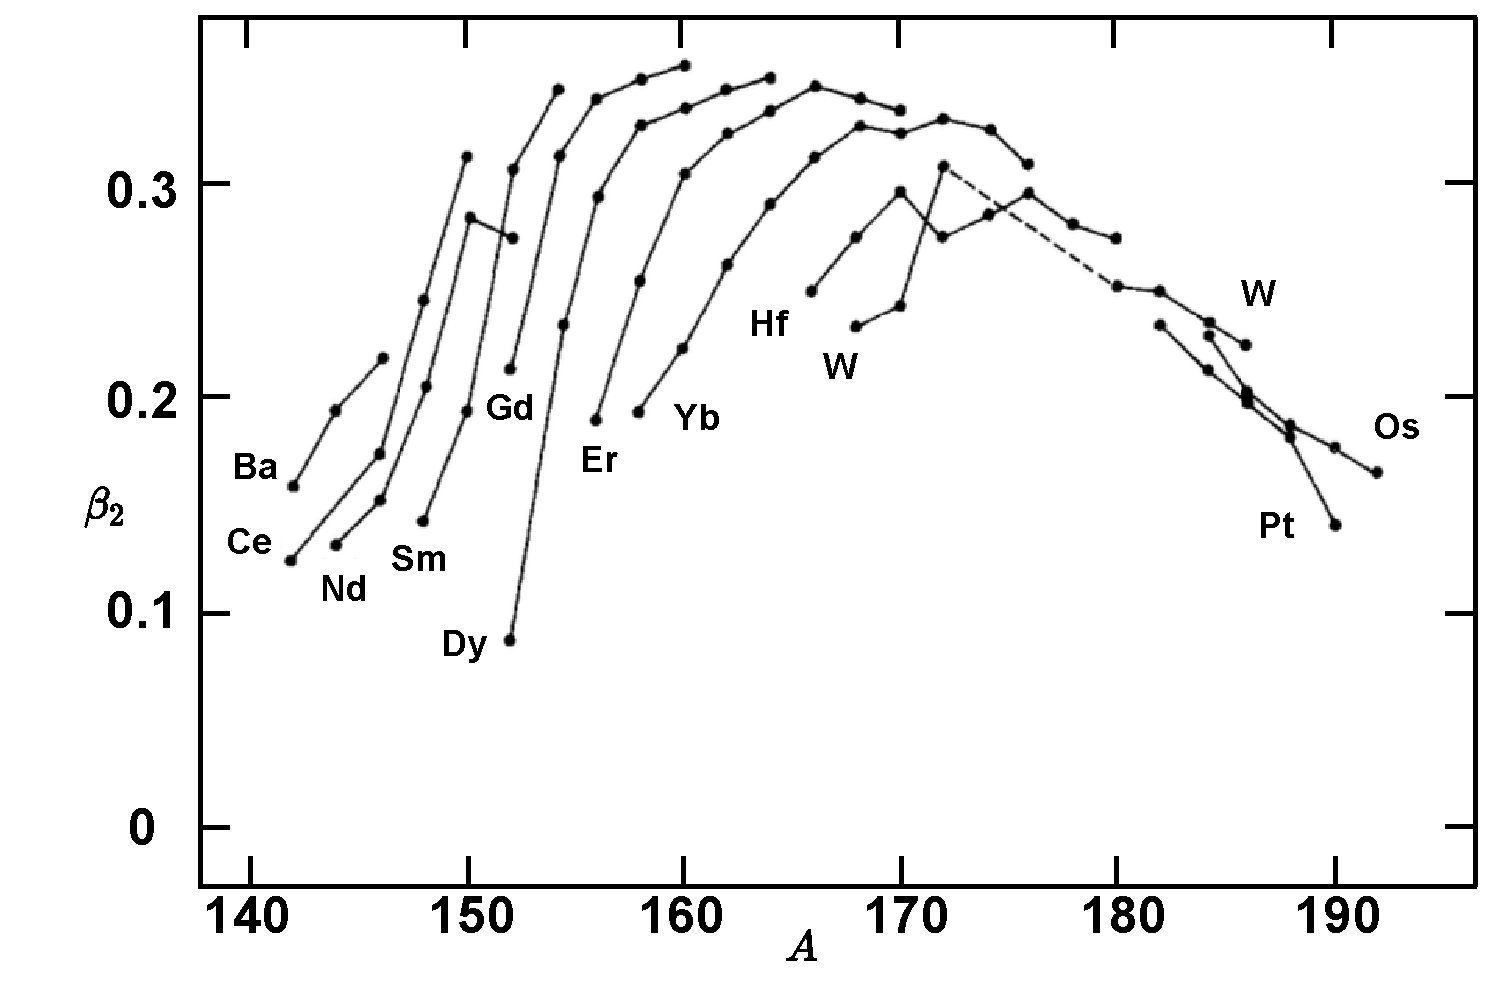
\includegraphics[scale=0.55]{Chapters/Figures/quadrupole_Deformation_rareEarth.pdf}
    \caption{Experimental values for the quadrupole deformation parameter $\beta_2$ as a function of the mass number $A$ for a few isotopes. The values of $\beta_2$ were determined from the experimental values $B(E2;0_i^+\to 0_f^+)$. Experimental data points were taken from Ref. \cite{krane1991introductory}.}
    \label{fig-quadrupole-beta-nuclides}
\end{figure}

In order to understand the behavior of $\beta$ shown in Fig. \ref{fig-quadrupole-beta-nuclides}, some shell model considerations need to be taken into account. Firstly, when deformation kicks in, the individual $j$ orbits within a major shell are nearly empty, resulting in positive values for the quadrupole moments of the nucleons from these orbits. With increasing deformation, large and positive values $Q(\beta)$ are present. Furthermore, as the shells start to fill, contributions from individual $j$ orbits to the total quadrupole moment will accumulate, making its value to decrease, vanish, and eventually becoming negative near the shell closure.

The \emph{observed} quadrupole moment (measured, also known as spectroscopic) can be obtained via a transformation to the laboratory frame applied to $Q_0$, meaning that the spectroscopic quadrupole moment has the result \cite{casten2000nuclear}:
\begin{align}
    Q_\text{spec}=Q_0\left[\frac{3K^2-I(I+1)}{(I+1)(2I+3)}\right]\ ,
    \label{quadrupole-moment-spectro}
\end{align}
where the quantum number $K$ is again the projection of $I$ onto the symmetry (deformation) axis. The dependence of $Q_\text{spec}$ on $K$ and $I$ emphasizes the fact that the \emph{observed} shape of the rotating nucleus is not equivalent to the shape in the intrinsic frame of reference.

Remarking the fact that when prolate nucleus rotates about an axis that is perpendicular to the symmetry axis, the \emph{averaged} density distribution of the nuclear matter will look more like an oblate shape (see Fig. \ref{fig-averaged-prolate-density} for a clearer picture). As a result, when the intrinsic quadrupole moment is positive, the observed one will have a negative value: for the condition $I(I+1)>3K^2$ taken from Eq. \ref{quadrupole-moment-spectro}.

\begin{figure}
    \centering
    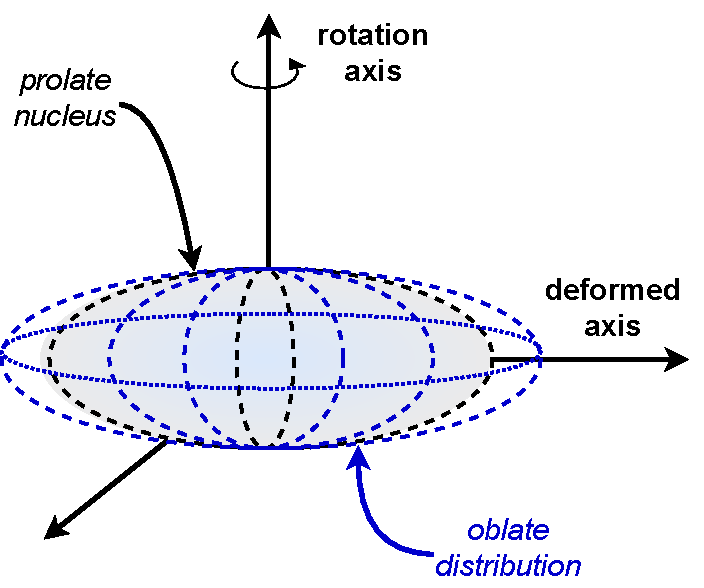
\includegraphics[scale=0.65]{Chapters/Figures/averaged_nuclearMatter_prolate.pdf}
    \caption{An example which aims at depicting an average flattened (oblate) density distribution that is generated by the rotation of a prolate nucleus. As the `initial' prolate nucleus with its nuclear density is distributed along the deformed axis exhibits rotation, the rotated shape will generate an averaged oblate disk along the rotation axis. This is why the observed quadrupole moment will have a negative sign if $Q_0>0$.}
    \label{fig-averaged-prolate-density}
\end{figure}

% The \emph{transition quadrupole moment} $Q_t$ is another quantity which can be determined from the lifetime measurement of excited states, and it is related to the intrinsic quadrupole moment via \cite{ayangeakaa2013exotic}:
% \begin{align}
%     Q_t(I+1)=\sqrt{Q_0(I)Q_0(I+2)}\ .
% \end{align}

Another important quantity that can be used as a `test' for collectivity and deformation within nuclei is the $E2$ transition probability (of electric quadrupole type). This is because the ground state of even-even nuclei is $0^+$ and the first excited state (typically $2^+$) can only decay via the electric quadrupole interaction (as $E2$ radiation \cite{casten2000nuclear}), meaning that deformation effects can be understand from these low-lying transitions. The general expression for calculating a transition `strength' is given in terms of the initial and final states \cite{matta2017exotic}:
\begin{align}
    B(E2;\ I_i\to I_f)=\frac{1}{2I_i+1}\left|\bra{\Psi_f}\left|\mathcal{M}(E2)\right|\ket{\Psi_i}\right|^2\ ,
    \label{eq-general-reduced-E2}
\end{align}
where the two wave-functions represent the initial and final state, respectively, and $\mathcal{M}(E2)$ is the quadrupole transition operator. In fact, Eq. \ref{eq-general-reduced-E2} tells that the reduced transition probabilities can be extracted from the `matrix elements' of the electric quadrupole operator. Equivalently, the reduced quadrupole transition probability $B(E2)$ can be given in terms of the Clebsch-Gordan coefficients \cite{bohr1998nuclear}:
\begin{align}
    B(E2;\ I_i\to I_f)=\frac{5}{16\pi}e^2Q_0^2\left|\bra{I_iK20}\ket{I_2K}\right|^2]\ ,
\end{align}
where the coefficient can also be written as $\bra{I_iK20}\ket{I_2K}\equiv C^{I_i2I_f}_{K0K}$. In the case of $0^+\to 2^+$, the reduced transition probability will be given by:
\begin{align}
    B(E2;\ 0^+\to 2^+)=\frac{5}{16\pi}e^2Q_0^2\ .
\end{align}

From the quadratic dependence of the intrinsic quadrupole moment on $\beta$, large values of $\beta$ that are specific to deformed nuclei ($\beta\approx 0.3$) will lead to values for $B(E2)$ which are one-two orders of magnitude higher than those specific to nearly spherical nuclei ($\beta\approx 0.05$). Such a systematic is the main cause why higher $B(E2)$ values indicate large nuclear deformations.

In nuclei, usually the valence nucleons are causing some core polarizations, which as a result will affect the `final' electric quadrupole moment. In fact, the single-particle quadrupole moment is given by the following expression:
\begin{align}
    Q_\text{sp}(j)=-\frac{2j-1}{2j+2}\frac{e_\text{eff}}{e}\langle r^2\rangle\ .
    \label{single-particle-quadrupole-moment}
\end{align}
The need for an \emph{effective charge} $e_\text{eff}$ is discussed in \cite{heyde1994nuclear}. The mean squared radius corresponds to the radial function of the nucleon within that $j$ orbital. Due to the nuclear energy being minimal (when discussing stable deformation) only if the overlap of the core with the valence particle is maximal, a particle+core interaction will produce an oblate polarization, driving the nucleus to a final oblate deformed state. The opposite is true for the hole+core coupling (see discussion made in \cite{neugart2006nuclear}).

An interesting characteristic which emerges from Eq. \ref{single-particle-quadrupole-moment} is the fact that besides even-even nuclei with $I=0$, odd-$A$ nuclei the total spin $I=\frac{1}{2}$ will be zero. The experimental data from Fig. \ref{experimental-Q-odd-nuclei} show the magnitude of $Q$ which would correspond to the value given by Eq. \ref{single-particle-quadrupole-moment}. One can see sharp increase with the nucleonic number for some nuclei (e.g., $^{175}$Lu or $^{167}$Er) but also very strong decrease to negative values (e.g., the isotope $^{123}$Sn). These alternations between positive (prolate) and negative (oblate) $Q$ values are also located near the magic numbers. Moreover, one should note that for the cases when the odd-particle is a neutron, the nucleus still exhibits a quadrupole moment that is different from zero, meaning that not only the last nucleon will be responsible for the quadrupole moment \cite{bertulani2007nuclear}.

\begin{figure}
    \centering
    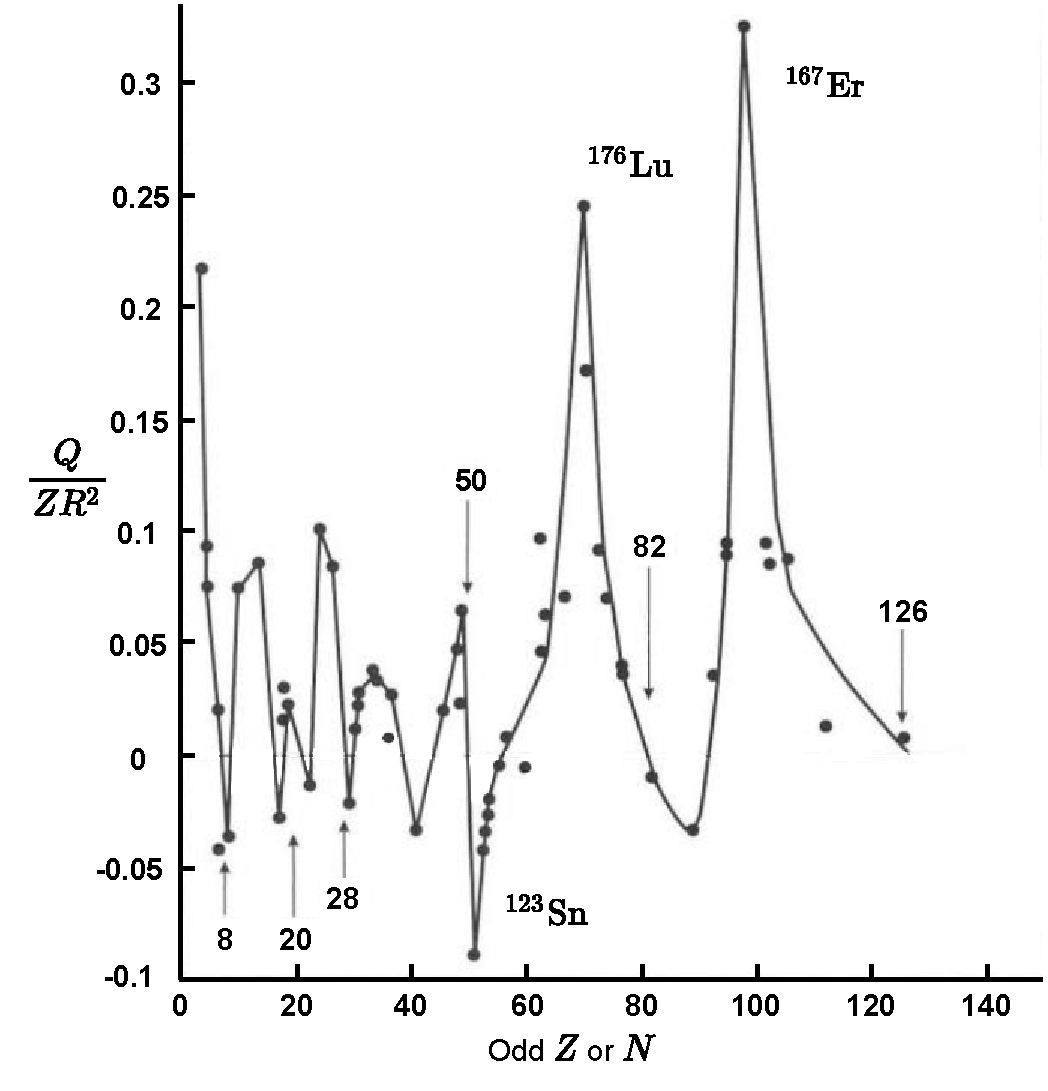
\includegraphics[scale=0.7]{Chapters/Figures/Exp_quadrupoleMoments.pdf}
    \caption{The measured quadrupole moments, given in units of $ZR^2$, as a function of the odd proton and neutron numbers $Z$,$N$, respectively. Experimental data are taken from Ref. \cite{bertulani2007nuclear}.}
    \label{experimental-Q-odd-nuclei}
\end{figure}

The experimental data for the measured $Q_\text{spec}$ values (the spectroscopic quadrupole moment in units of \emph{barn}) for the lowest $2^+$ states of even-$Z$ and even-$N$ nuclei is also graphically represented in Fig. \ref{experimental-quadrupole-2Plus-states}, where both positive and negative values are observed. As already explained, a negative value for $Q_\text{spec}$ (say for example $Q_\text{spec}=-2$ b, for nuclei with stable permanent deformation which belong to the mass range $150\leq A \leq 190$) will correspond to an intrinsic quadrupole moment $Q_0=7$ b. This will correspond to a quadrupole deformation parameter $\beta\approx 0.29$. Such values indicate substantial eccentricities of the nuclear matter.

\begin{figure}
    \centering
    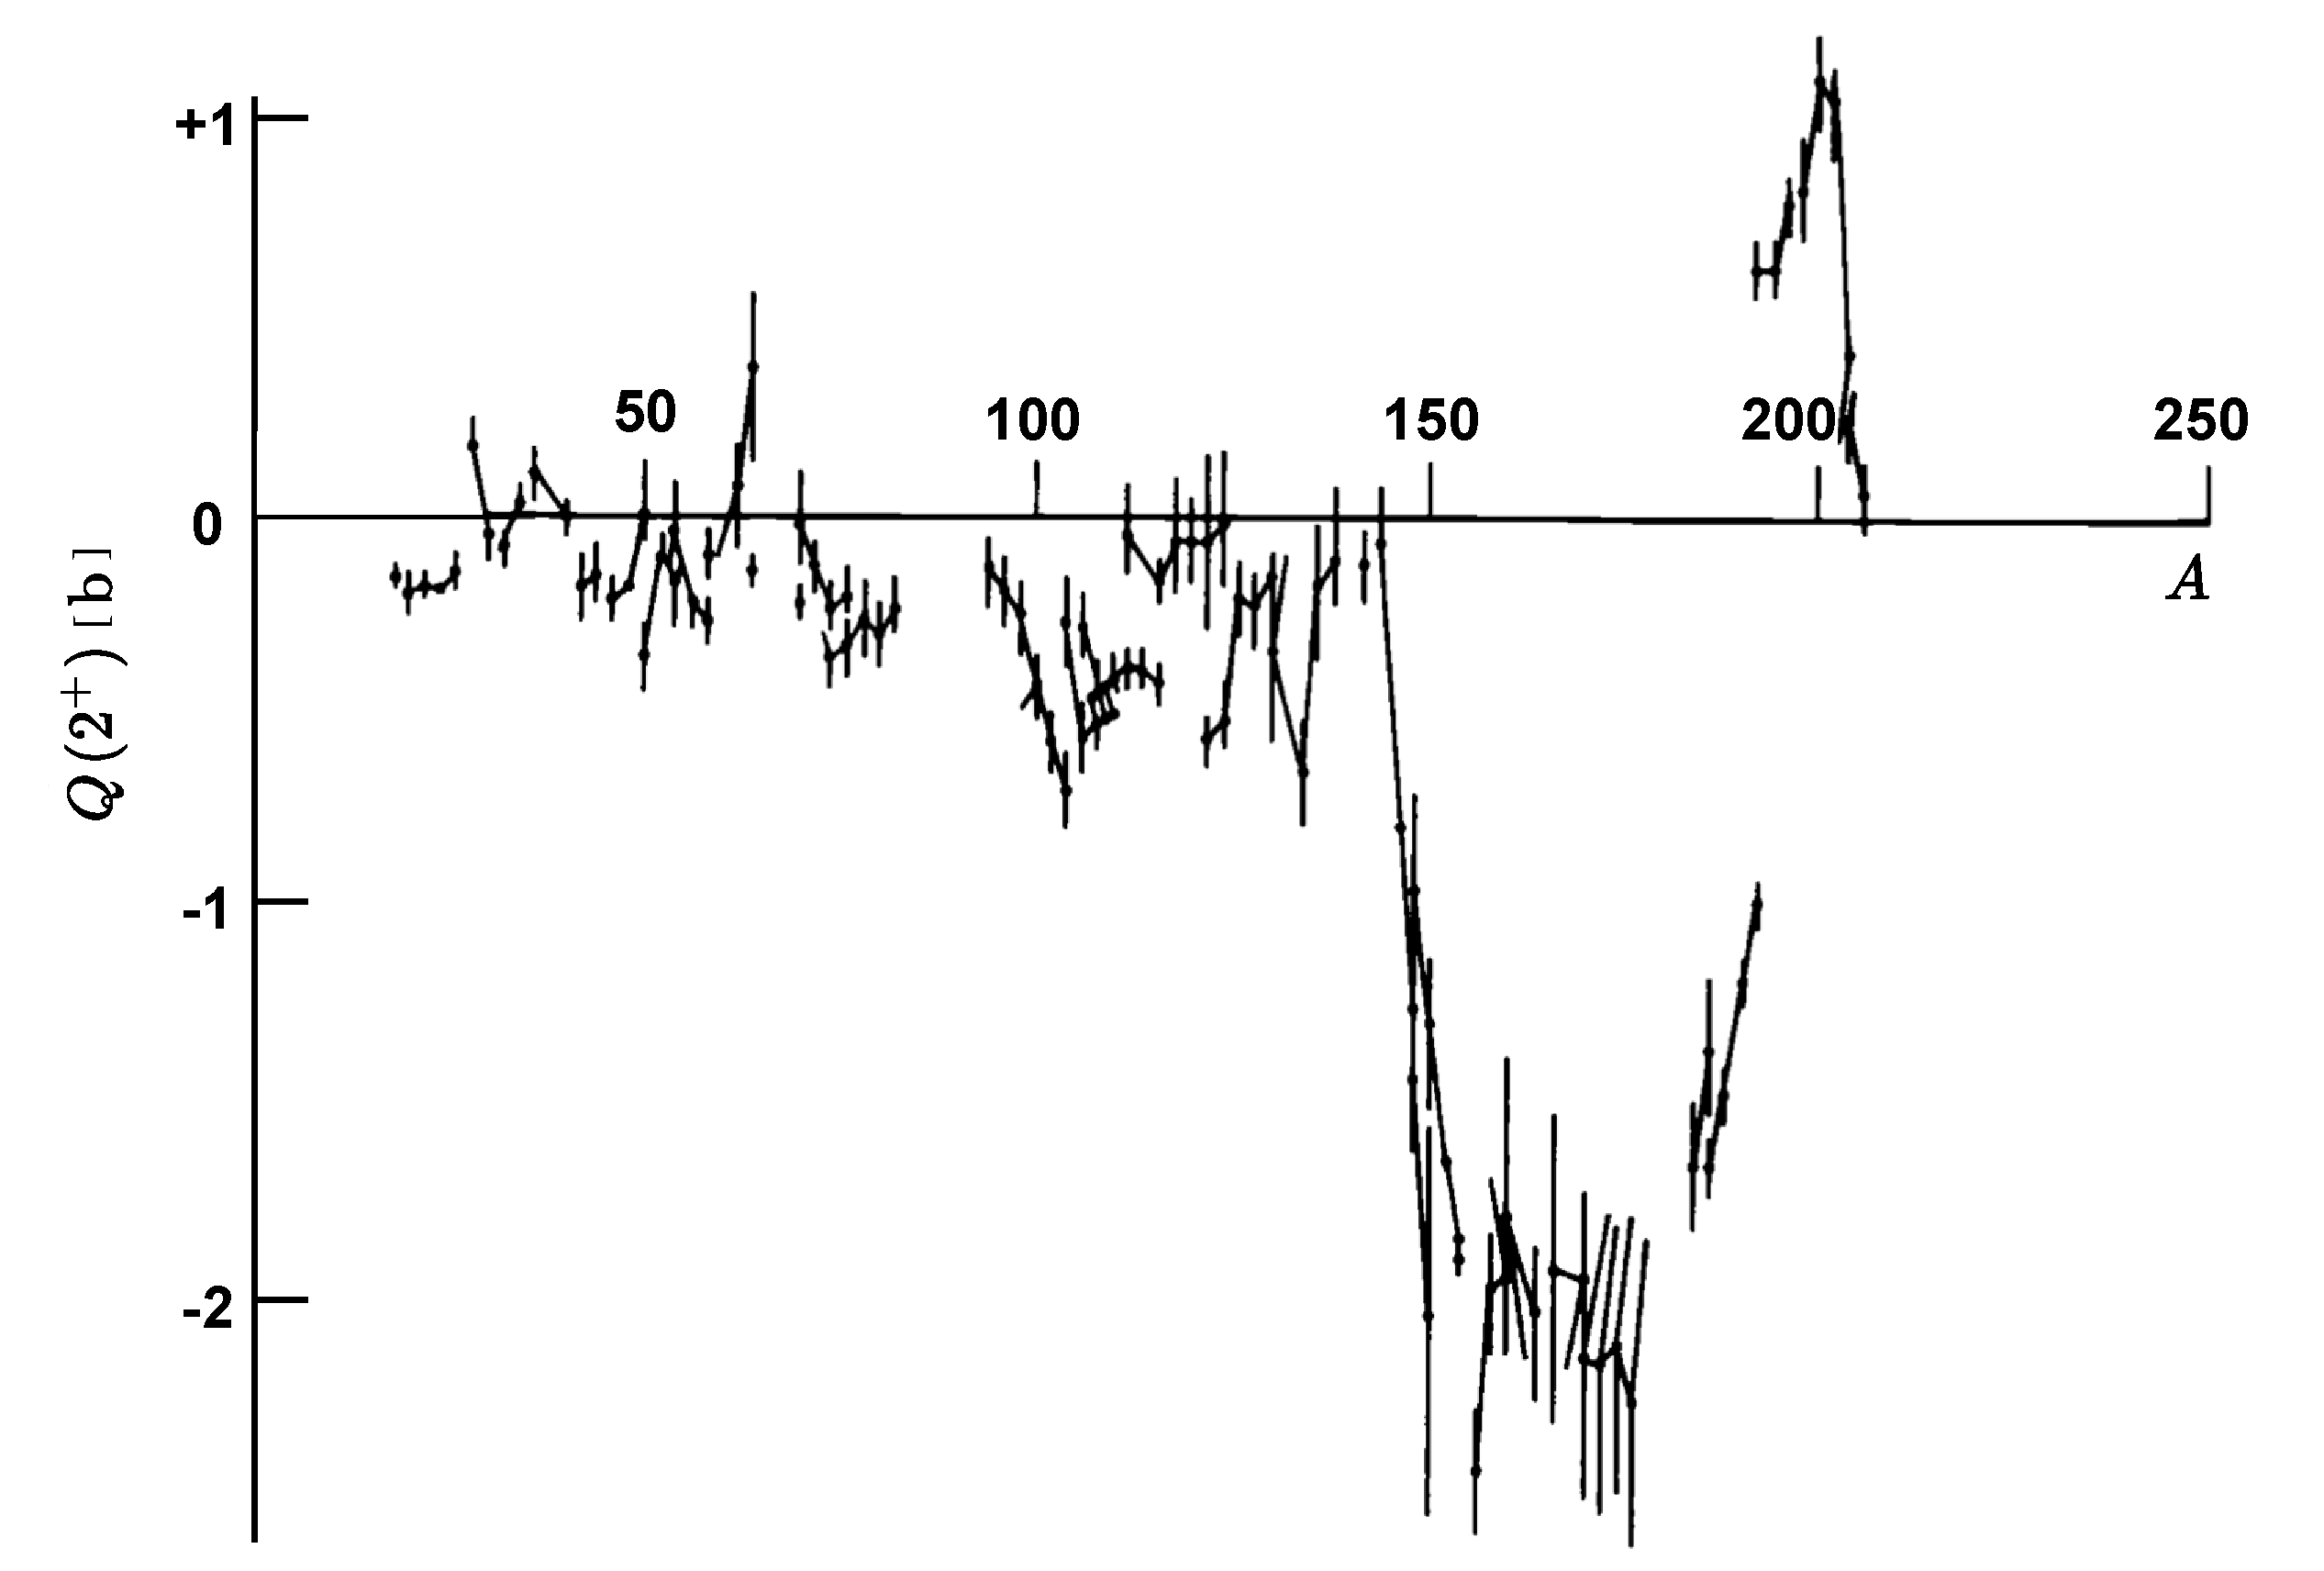
\includegraphics[scale=0.33]{Chapters/Figures/2Plus_spectroscopicQ.pdf}
    \caption{The measured quadrupole moment $Q_\text{spec}$ as defined in Eq. \ref{quadrupole-moment-spectro} for the first excited $2^+$ states in even-even nuclei. The lines between data-points connect the isotope sequences. The figure was reproduced with the experimental data from \cite{krane1991introductory}.}
    \label{experimental-quadrupole-2Plus-states}
\end{figure}